\newpage
\chapter{METODE PENELITIAN} \label{Bab III}

\section{Alur Penelitian} \label{III.Alur}
Pada penelitian ini, alur penelitian yang digunakan yang digunakan dalam identifikasi mineral kasiterit pada citra mikroskop menggunakan \textit{Mask} R-CNN ditunjukkan pada Gambar \ref{fig:3.alur}. \par

\begin{figure}[H]
    \centering
    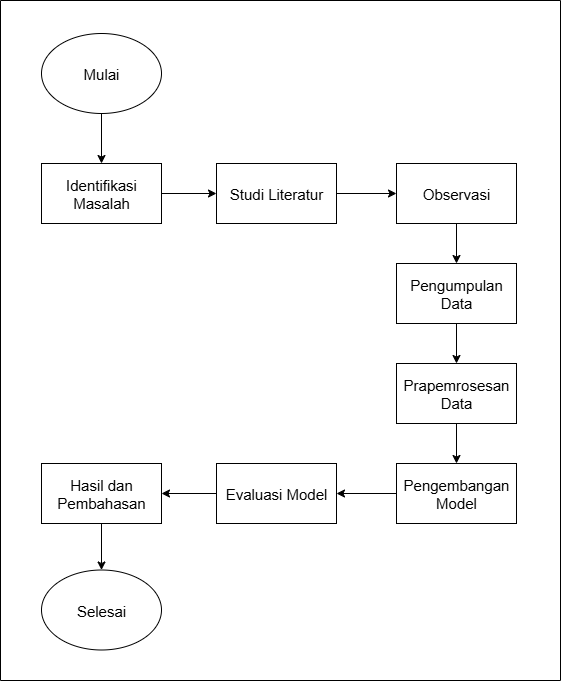
\includegraphics[width=0.9\textwidth]{figure/alurPenelitian.png}
    \caption{Alur Penelitian}
    \label{fig:3.alur}
\end{figure}

\section{Penjabaran Langkah Penelitian} \label{III.Jabar Alur}
Pada alur penelitian yang ditunjukkan pada Gambar \ref{fig:3.alur}, berikut merupakan penjabaran mengenai langkah penelitian yang dilakukan. \par

\subsection{Identifikasi Masalah} \label{III.LangkahIdentifikasiMasalah}
Pada tahap identifikasi masalah ditemukan bahwa proses identifikasi mineral kasiterit di Laboratorium Eksplorasi PT. Timah Tbk. masih dilakukan secara manual menggunakan metode \textit{Grain Counting Analysis} (GCA) dengan bantuan mikroskop binokuler. Metode ini membutuhkan ketelitian dan pengalaman tinggi dari analis, karena setiap butiran mineral harus diamati dan dihitung satu per satu secara visual. Pendekatan tersebut memiliki keterbatasan seperti memerlukan waktu yang lama, bersifat subjektif, serta rentan terhadap kesalahan pengamatan akibat kelelahan visual. Selain itu, keberadaan butiran mineral yang saling tumpang tindih (\textit{occluded}) juga menyebabkan kesulitan dalam membedakan batas antar butir kasiterit, sehingga dapat menurunkan akurasi hasil identifikasi. Oleh karena itu, penelitian ini berfokus untuk mengembangkan metode identifikasi mineral kasiterit menggunakan model \textit{Mask} R-CNN yang dapat melakukan segmentasi dengan menerapkan teknik \textit{amodal instance segmentation}, sehingga dapat digunakan untuk mengidentifikasi dan melakukan segmentasi bentuk utuh butir mineral kasiterit meskipun terjadi tumpang tindih antar butir pada citra mikroskop. \par

\subsection{Studi Literatur} \label{III.LangkahStudiLiteratur}
Pada tahap ini dilakukan pengumpulan berbagai macam informasi, referensi, konsep dasar, serta teori yang menjadi landasan dilakukannya penelitian ini. Proses ini dilakukan dengan mencari referensi berupa buku, jurnal, penelitian terdahulu, publikasi ilmiah, maupun sumber terpercaya lainnya yang berkaitan dengan penerapan \textit{deep learning} dalam bidang geologi, khususnya pada identifikasi mineral menggunakan citra mikroskop. Fokus kajian diarahkan pada pemahaman arsitektur \textit{Mask} R-CNN serta penerapan teknik \textit{amodal instance segmentation} yang digunakan untuk mengidentifikasi bentuk utuh butir mineral kasiterit meskipun terjadi tumpang tindih antar butir pada citra mikroskop. \par

\subsection{Observasi} \label{III.LangkahObservasi}
Kegiatan observasi dilakukan secara langsung di Laboratorium Eksplorasi PT. Timah Tbk. sebagai bagian dari proses pengumpulan data dan pemahaman terhadap sistem identifikasi mineral yang sedang diterapkan. Dalam kegiatan ini, peneliti melakukan kunjungan langsung ke laboratorium untuk melihat secara nyata proses identifikasi mineral menggunakan mikroskop yang menjadi bagian penting dari analisis mineralogi. Observasi dilakukan dengan tujuan untuk memahami kondisi aktual pelaksanaan analisis mineral di lapangan serta memperoleh gambaran awal mengenai metode yang digunakan dalam kegiatan laboratorium. \par

Selama kegiatan observasi, peneliti berkesempatan untuk melakukan wawancara langsung dengan Bapak Mesa Madestriasa selaku Kepala Laboratorium Eksplorasi PT. Timah Tbk. Wawancara ini bertujuan untuk memperoleh informasi terkait mekanisme identifikasi mineral kasiterit yang sedang diterapkan, permasalahan yang dihadapi selama proses analisis, serta faktor-faktor yang memengaruhi keakuratan hasil pengamatan mikroskopis. Dari hasil wawancara, diketahui bahwa kegiatan identifikasi mineral di laboratorium masih dilakukan secara manual dengan tingkat ketergantungan tinggi terhadap kemampuan dan ketelitian analis. Metode tersebut memerlukan waktu cukup lama dan rawan menghasilkan variasi hasil identifikasi antar pengamat akibat faktor kelelahan visual maupun subjektivitas pengamatan. Gambar \ref{fig:Wawancara} pada Lampiran \ref{lampiran:Wawancara} merupakan dokumentasi kegiatan wawancara yang dilakukan oleh peneliti bersama Kepala Laboratorium Eksplorasi PT. Timah Tbk. sebagai bagian dari proses pengumpulan data penelitian. \par

Selain melakukan wawancara, peneliti juga mendapatkan kesempatan untuk mencoba secara langsung penggunaan mikroskop binokuler yang digunakan dalam proses identifikasi mineral. Kegiatan ini didampingi oleh salah satu tim analis di Laboratorium Eksplorasi PT. Timah Tbk. Selama pengamatan, peneliti mempelajari karakteristik visual mineral kasiterit seperti bentuk, warna, kilap, dan reflektivitasnya, serta membandingkannya dengan mineral ikutan lain yang sering muncul bersamaan pada sampel. Pengalaman langsung ini memberikan pemahaman yang lebih konkret mengenai tantangan identifikasi butiran mineral, terutama ketika butiran tersebut saling menutupi atau mengalami oklusi sebagian. Lampiran \ref{lampiran:Observasi} merupakan kumpulan dokumentasi hasil observasi yang dilakukan peneliti di Laboratorium Eksplorasi PT. Timah Tbk., yang menampilkan proses identifikasi mineral serta kondisi lingkungan penelitian secara langsung. \par

Berdasarkan hasil wawancara dan pengamatan tersebut, dapat disimpulkan bahwa metode manual yang diterapkan di laboratorium memiliki keterbatasan dalam hal efisiensi dan objektivitas. Kondisi ini menjadi dasar kuat bagi peneliti untuk mengembangkan pendekatan otomatis berbasis teknologi \textit{deep learning} menggunakan model \textit{Mask Region-based Convolutional Neural Network} (\textit{Mask} R-CNN). Model ini dipilih karena mampu melakukan deteksi dan segmentasi setiap butir mineral kasiterit secara presisi, bahkan dengan menerapkan teknik \textit{amodal instance segmentation} untuk merekonstruksi bentuk utuh mineral yang sebagian tertutup oleh butir lainnya. \par

Setelah kegiatan wawancara dan observasi selesai dilakukan, peneliti mengurus proses administratif berupa pengajuan surat pengantar resmi sebagai bentuk permohonan izin penelitian kepada pihak laboratorium. Surat ini digunakan sebagai dasar legalitas untuk memperoleh data citra mikroskop yang akan digunakan dalam penelitian. Gambar \ref{fig:SuratIzinPenelitian} pada Lampiran \ref{lampiran:SuratIzin} merupakan hasil dari Surat Permohonan Izin Penelitian Tugas Akhir yang telah dibuat dan disetujui oleh pihak Fakultas Teknologi Industri, Institut Teknologi Sumatera sebagai dasar pelaksanaan kegiatan penelitian di PT. Timah Tbk.\par

\subsection{Pengumpulan Data} \label{III.LangkahPengumpulanData}
Data yang digunakan dalam penelitian ini berupa citra mikroskop mineral kasiterit yang merupakan data sekunder yang berasal dari Laboratorium Eksplorasi PT. Timah Tbk. Data tersebut diperoleh melalui Bapak Mesa Madestriasa selaku Kepala Laboratorium Eksplorasi PT. Timah Tbk. Gambar \ref{fig:PengumpulanData} pada Lampiran \ref{lampiran:Dataset} merupakan dokumentasi proses pengumpulan data yang dilakukan bersama Bapak Mesa Madestriasa. Proses ini dilakukan untuk memperoleh data pendukung penelitian berupa citra mikroskop yang telah dikumpulkan dan disimpan oleh pihak laboratorium. \par

Data yang didapatkan terdiri merupakan data citra mikroskop dengan berbagai mineral dan yang di gunakan sebanyak 142 citra mikroskop. % mencakup 7664 butir mineral kasiterit. 
Contoh citra pada dataset ditunjukkan pada Gambar \ref{fig:3.ContohDataset}. Gambar \ref{fig:PengantarPenelitian} pada Lampiran \ref{lampiran:SuratIzin} merupakan dokumentasi proses penyerahan surat izin penelitian oleh peneliti kepada Kepala Laboratorium Eksplorasi PT. Timah Tbk. sebagai bentuk permohonan resmi untuk pelaksanaan kegiatan penelitian di lingkungan laboratorium. \par

\begin{figure}[H] % Kalau menggunakan H, posisi gambar akan tepat dibawah teks
    \centering
    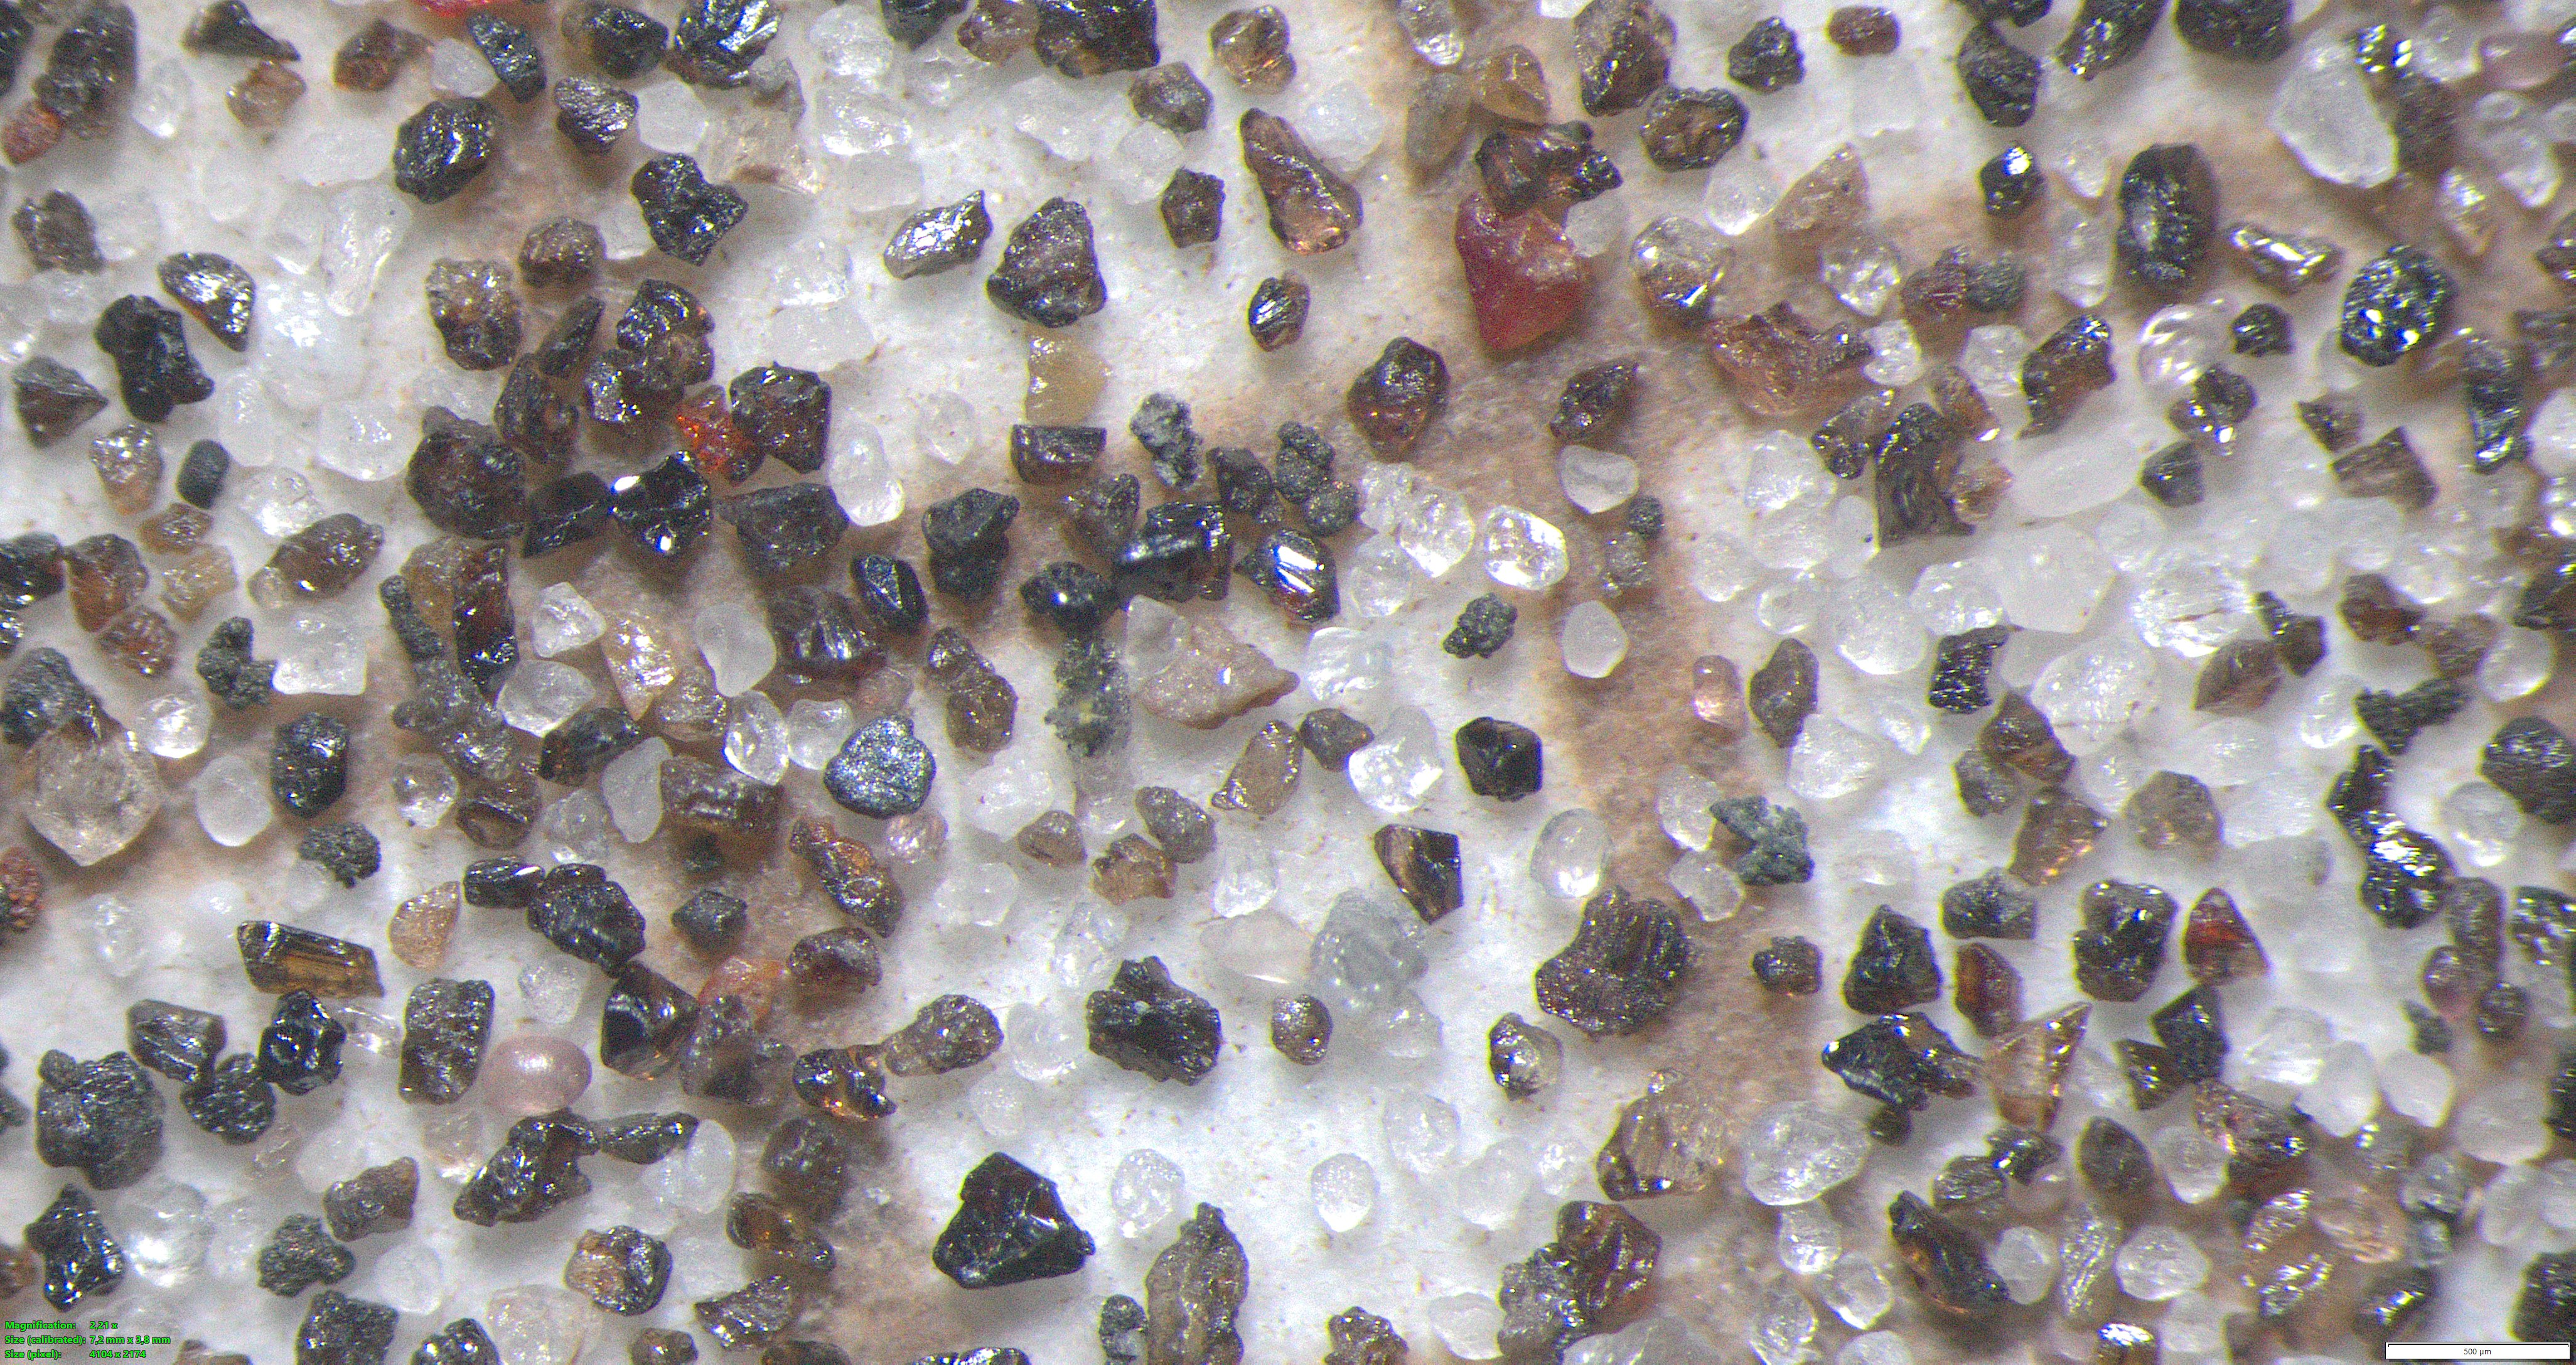
\includegraphics[width=1\textwidth]{figure/748-30100H.jpg}
    \caption{Contoh Gambar Dataset}
    \label{fig:3.ContohDataset}
\end{figure}

\subsection{Prapemrosesan Data} \label{III.LangkahPrapemrosesanData}
Pada penelitian ini, tahap prapemrosesan data dilakukan untuk mempersiapkan citra agar sesuai dengan kebutuhan model \textit{Mask} R-CNN. Tahap prapemrosesan meliputi pemilihan data untuk memastikan kualitas citra yang memadai, anotasi dan segmentasi data yang bertujuan untuk menandai serta memisahkan area objek kasiterit pada citra mikroskop, pembagian citra (\textit{image tiling}) yang digunakan untuk memecah citra menjadi beberapa bagian agar sesuai dengan kebutuhan input model, augmentasi data berupa \textit{flip} untuk membalik citra secara horizontal atau vertikal, \textit{rotate} untuk memutar citra pada sudut tertentu guna menambah variasi data, serta penambahan \textit{Gaussian noise} untuk meningkatkan ketahanan model terhadap gangguan visual, dan \textit{normalization} untuk menyesuaikan rentang nilai piksel citra agar berada dalam skala tertentu sehingga mempercepat konvergensi model. \par

\subsubsection{Pemilihan Data}
Dalam tahap prapemrosesan data, dilakukan proses pemilihan citra mikroskop untuk memastikan bahwa hanya citra dengan kualitas visual yang memadai yang digunakan dalam penelitian. Pemilihan ini mempertimbangkan beberapa faktor penting, termasuk tingkat pencahayaan serta kejelasan keberadaan objek mineral kasiterit pada citra mikroskop. Selain itu, citra yang tidak mengandung mineral kasiterit sebagai objek utama penelitian dikeluarkan dari proses selanjutnya. Citra dengan pencahayaan yang kurang memadai seperti pada Gambar \ref{fig:3.MilihGelap}, citra yang tidak menampilkan mineral kasiterit secara jelas seperti pada Gambar \ref{fig:3.MilihKurangJelas}, maupun citra yang tidak mengandung kasiterit seperti pada Gambar \ref{fig:3.MilihZircon}, dianggap tidak memenuhi kriteria kualitas data.

Berdasarkan proses seleksi tersebut, diperoleh sebanyak 142 citra mikroskop yang telah dinilai layak dan representatif oleh tim analis di Laboratorium Eksplorasi PT. Timah Tbk. untuk digunakan pada tahap pelatihan dan evaluasi model. Contoh citra yang memenuhi kriteria kelayakan ditunjukkan pada Gambar \ref{fig:3.MilihBagus}, sedangkan perbandingan tingkat keoptimalan kualitas citra secara keseluruhan dapat dilihat pada Gambar \ref{fig:3.MilihComparison}. Proses pemilihan ini bertujuan untuk memastikan bahwa data yang digunakan memiliki kualitas visual yang konsisten serta mencerminkan karakteristik objek penelitian secara akurat. Selain itu, proses kurasi ini dapat membatasi kemampuan model untuk beradaptasi terhadap citra dunia nyata yang memiliki kualitas pencahayaan atau kejernihan yang kurang ideal.

\begin{figure}[H]
    \centering
    % Baris pertama: dua gambar sejajar
    \begin{subfigure}[b]{0.475\textwidth}
        \centering
        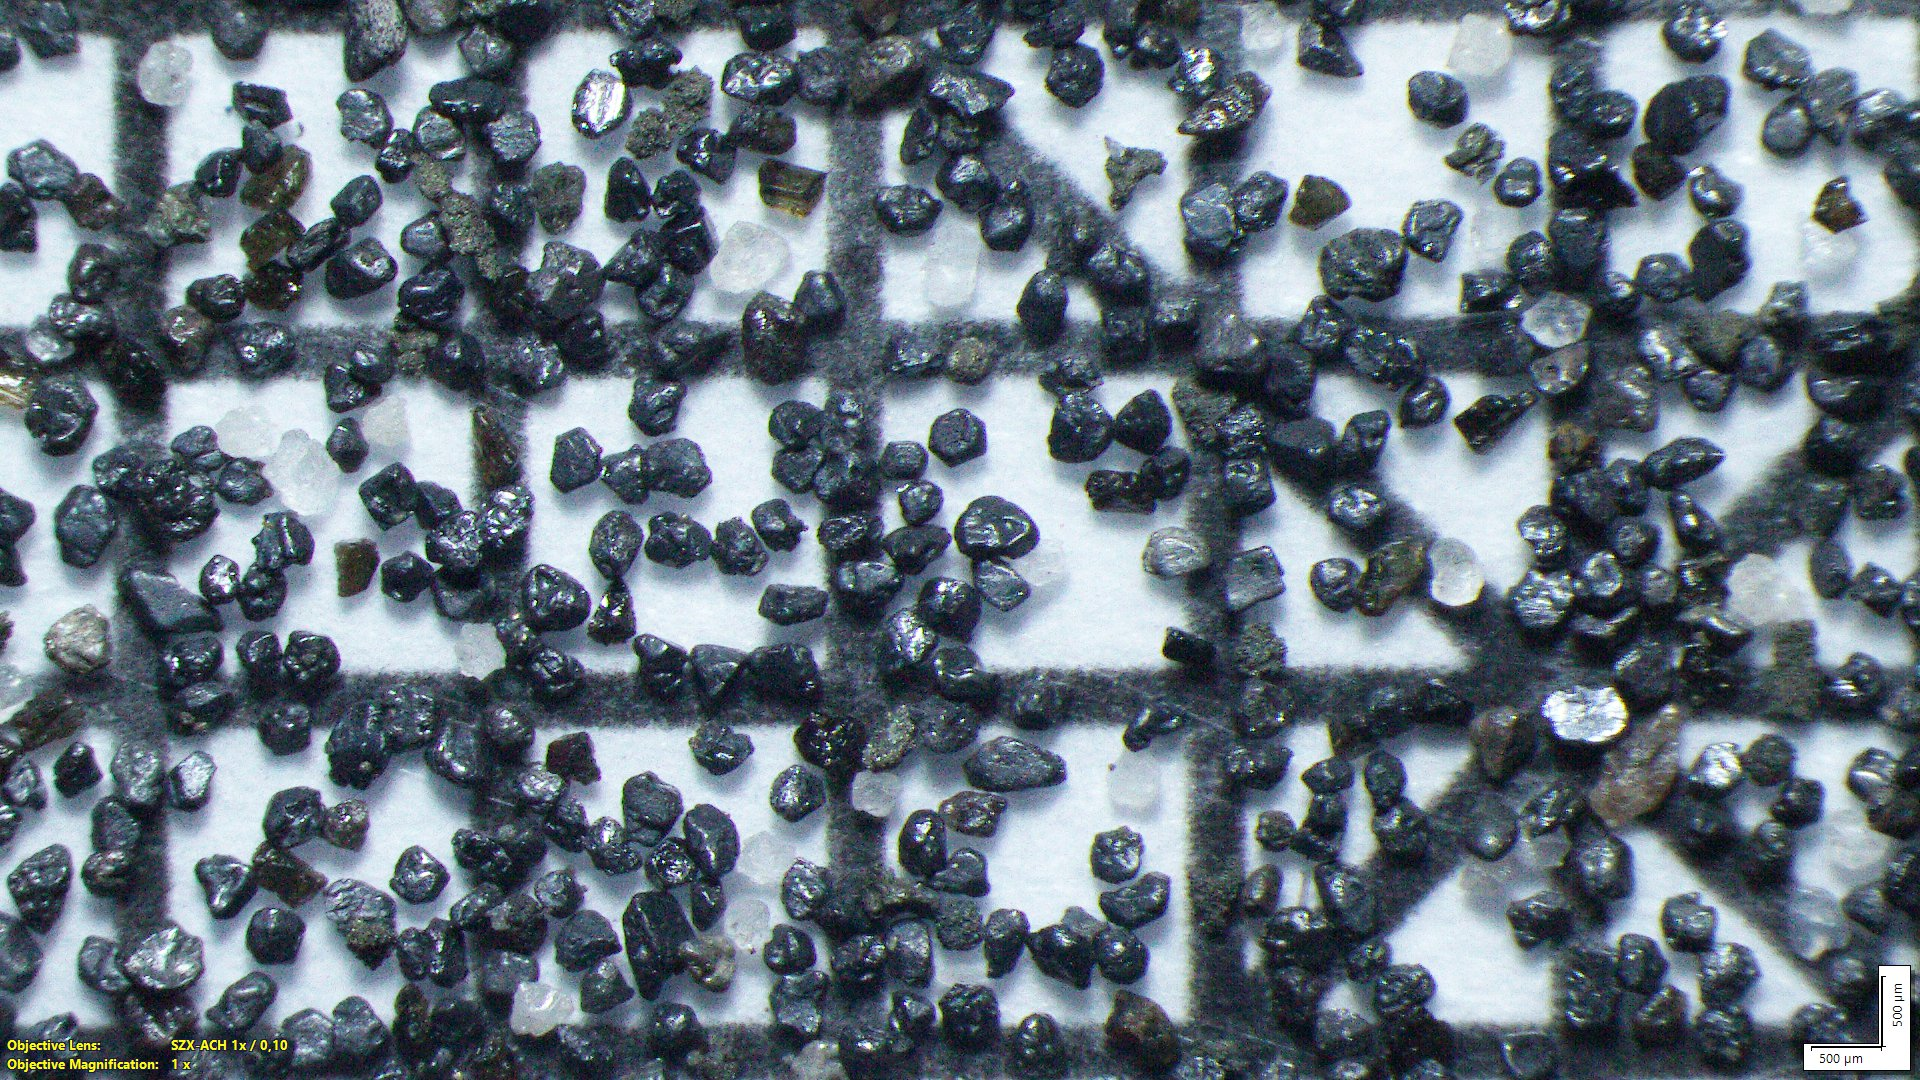
\includegraphics[width=\textwidth]{figure/MilihGelap.jpg}
        \caption{Citra dengan pencahayaan yang kurang memadai (Gelap)}
        \label{fig:3.MilihGelap}
    \end{subfigure}
    \hfill
    \begin{subfigure}[b]{0.475\textwidth}
        \centering
        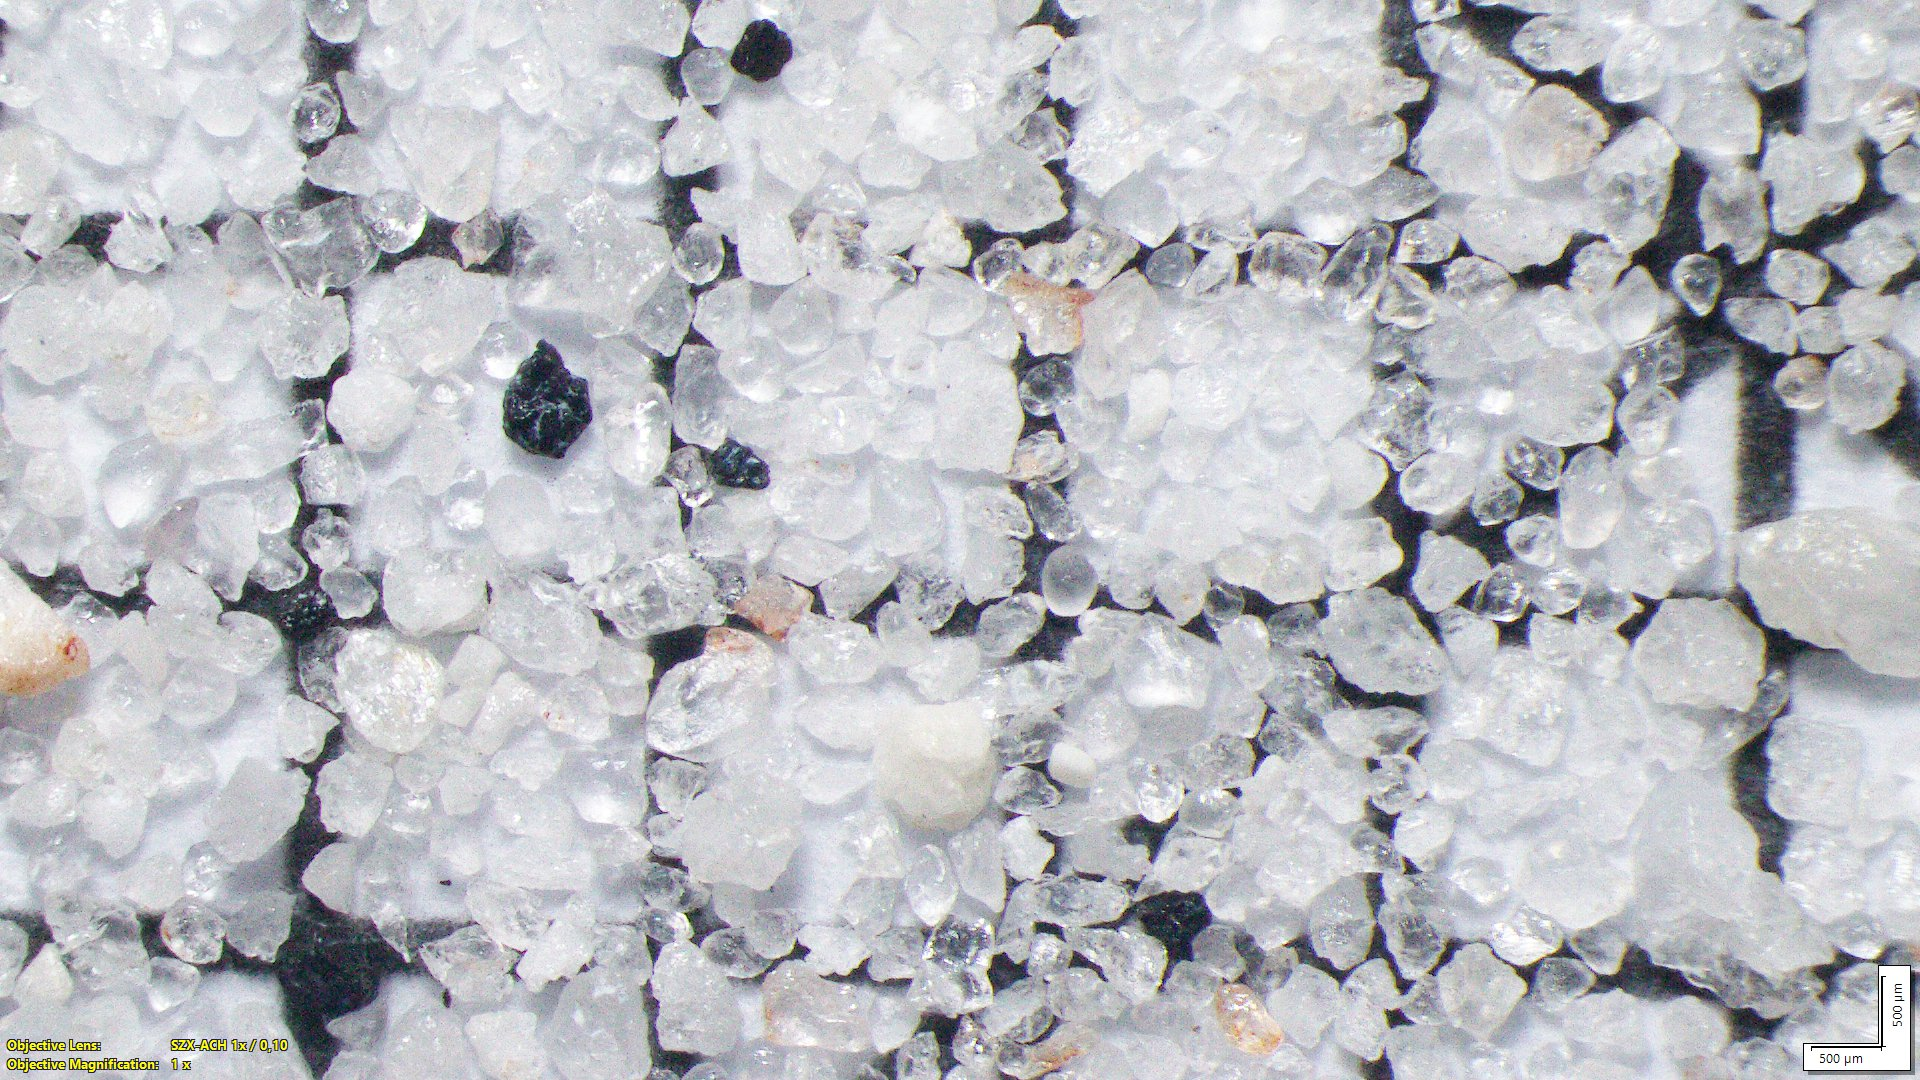
\includegraphics[width=\textwidth]{figure/MilihKurangJelas.jpg}
        \caption{Citra tidak menunjukkan keberadaan mineral target secara jelas}
        \label{fig:3.MilihKurangJelas}
    \end{subfigure}
    
    % Baris kedua: satu gambar di bawah tengah
    \vskip\baselineskip
    \begin{subfigure}[b]{0.475\textwidth}
        \centering
        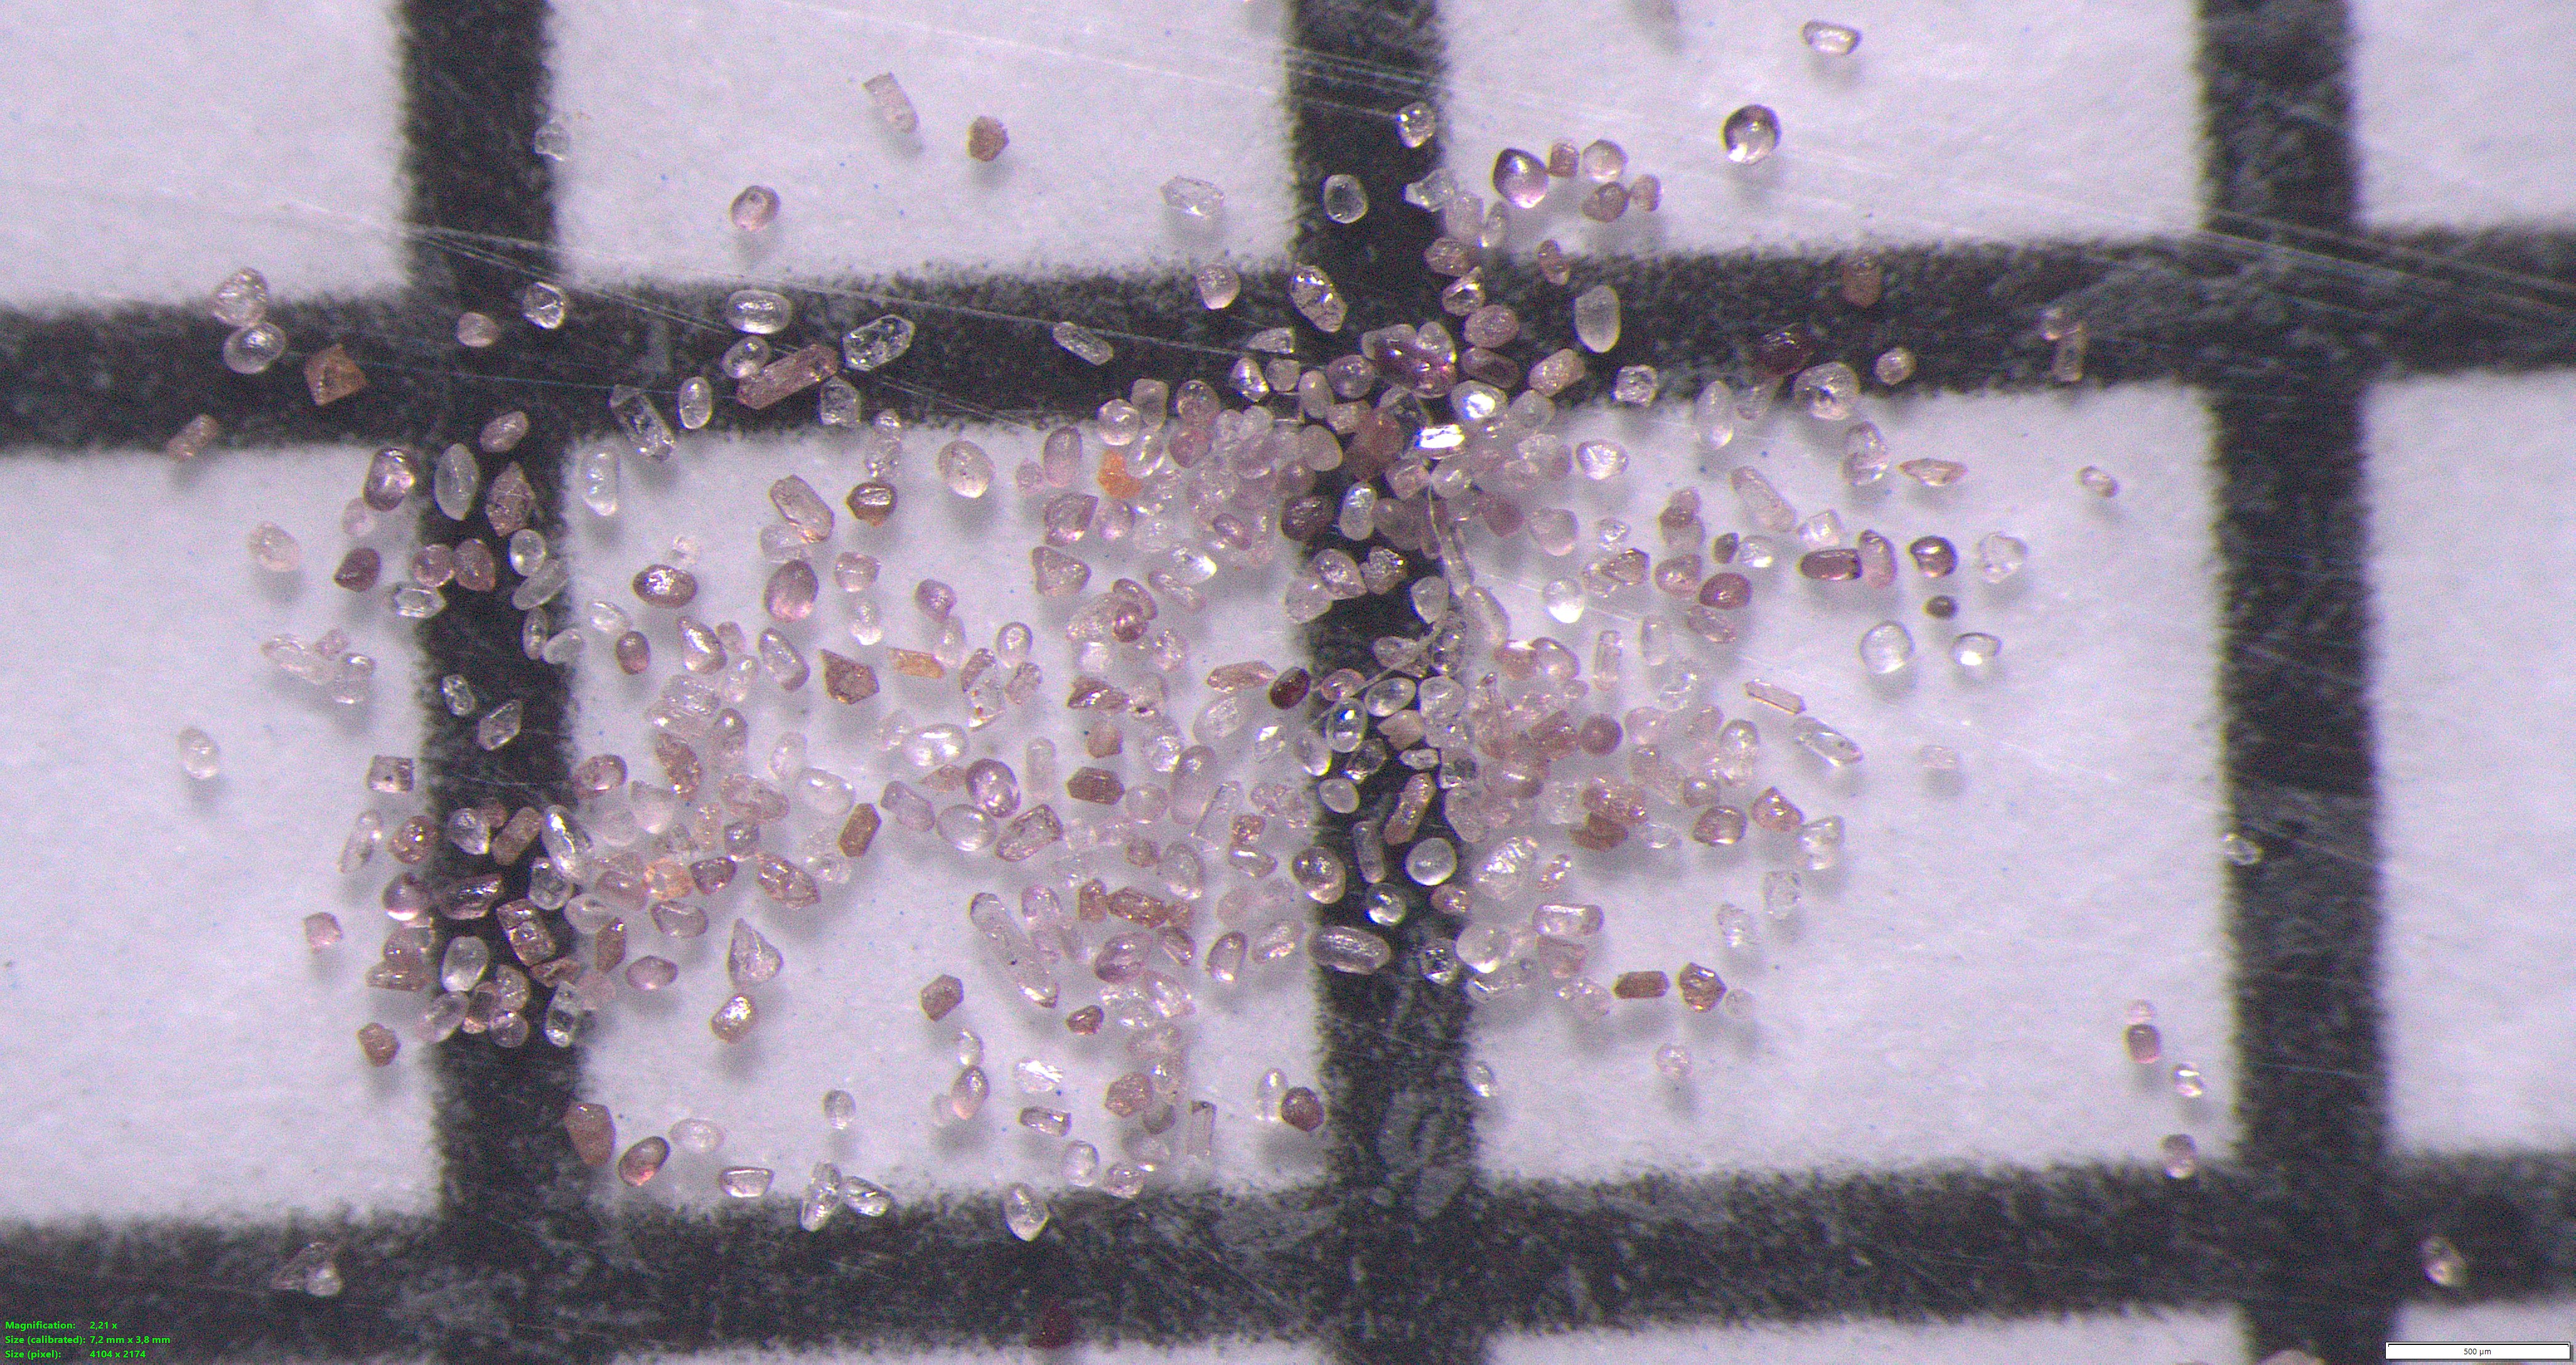
\includegraphics[width=\textwidth]{figure/MilihZircon.jpg}
        \caption{Citra yang tidak mengandung mineral kasiterit}
        \label{fig:3.MilihZircon}
    \end{subfigure}
    \hfill
    \begin{subfigure}[b]{0.475\textwidth}
        \centering
        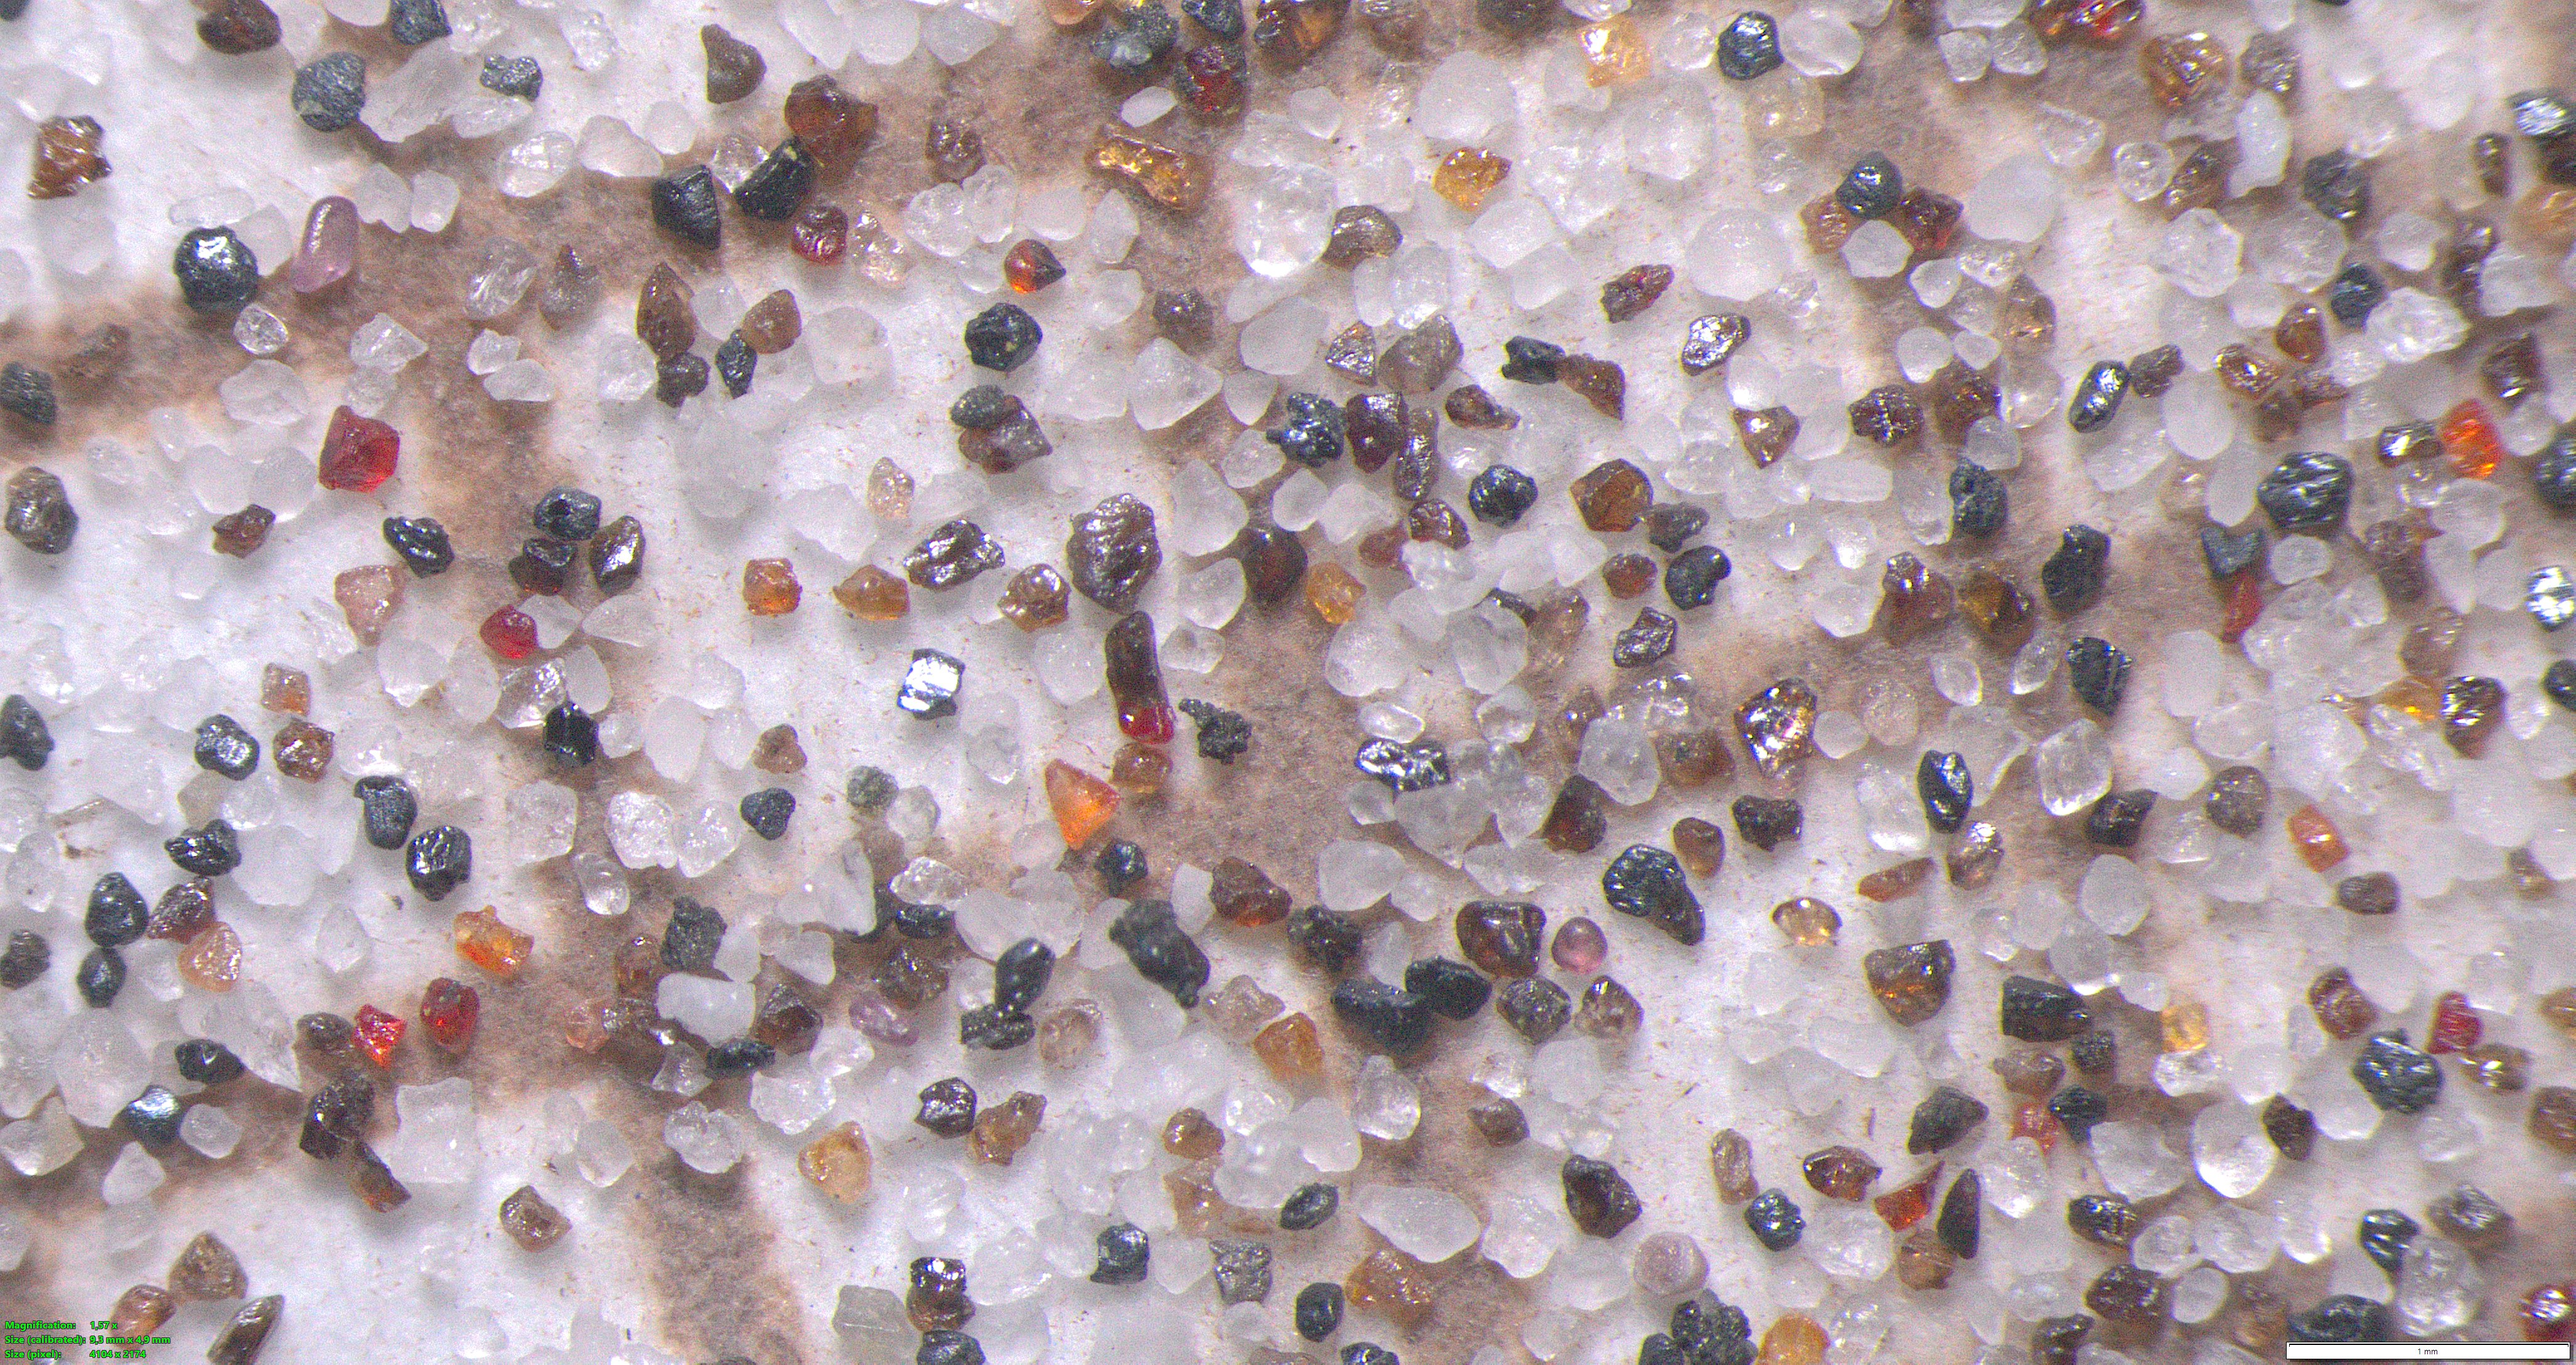
\includegraphics[width=\textwidth]{figure/MilihBagus.jpg}
        \caption{Citra pencahayaan dan kejelasannya optimal}
        \label{fig:3.MilihBagus}
    \end{subfigure}
    
    \caption{Perbandingan Tingkat Keoptimalan Data Citra Mikroskop}
    \label{fig:3.MilihComparison}
\end{figure}

\subsubsection{Anotasi Data}
Dalam proses anotasi data ini, peneliti terlebih dahulu melibatkan seorang anotator serta validator yang merupakan salah satu dari tim analis di Laboratorium Eksplorasi PT. Timah Tbk. untuk mengerjakan 10 citra mikroskop sebagai anotasi awal. Hasil dari anotasi tersebut kemudian dipelajari oleh peneliti untuk memahami pola dan standar anotasi yang telah ditetapkan. Setelah itu, peneliti melanjutkan proses anotasi secara mandiri terhadap 132 citra mikroskop tambahan. Seluruh hasil anotasi tersebut kemudian dievaluasi kembali oleh anotator yang sama guna memastikan konsistensi dan ketepatan anotasi. Proses evaluasi dilakukan dengan memberikan koreksi menggunakan warna berbeda, seperti warna merah untuk anotasi awal dan hijau untuk koreksi, sehingga perbedaan dapat teridentifikasi secara visual seperti yang terlihat pada Gambar \ref{fig:3.AnotasiAwal} dan Gambar \ref{fig:3.AnotasiEval}. Dokumentasi dari proses ini mencerminkan perbandingan antara hasil anotasi awal dengan hasil yang telah diperiksa, sekaligus menjadi bukti adanya proses revisi dan penyempurnaan. Contoh hasil anotasi data ditunjukkan pada Gambar \ref{fig:3.HasilAnotasiData} berikut.\par

\begin{figure}[H]
    \centering
    % Baris pertama: dua gambar sejajar
    \begin{subfigure}[b]{0.475\textwidth}
        \centering
        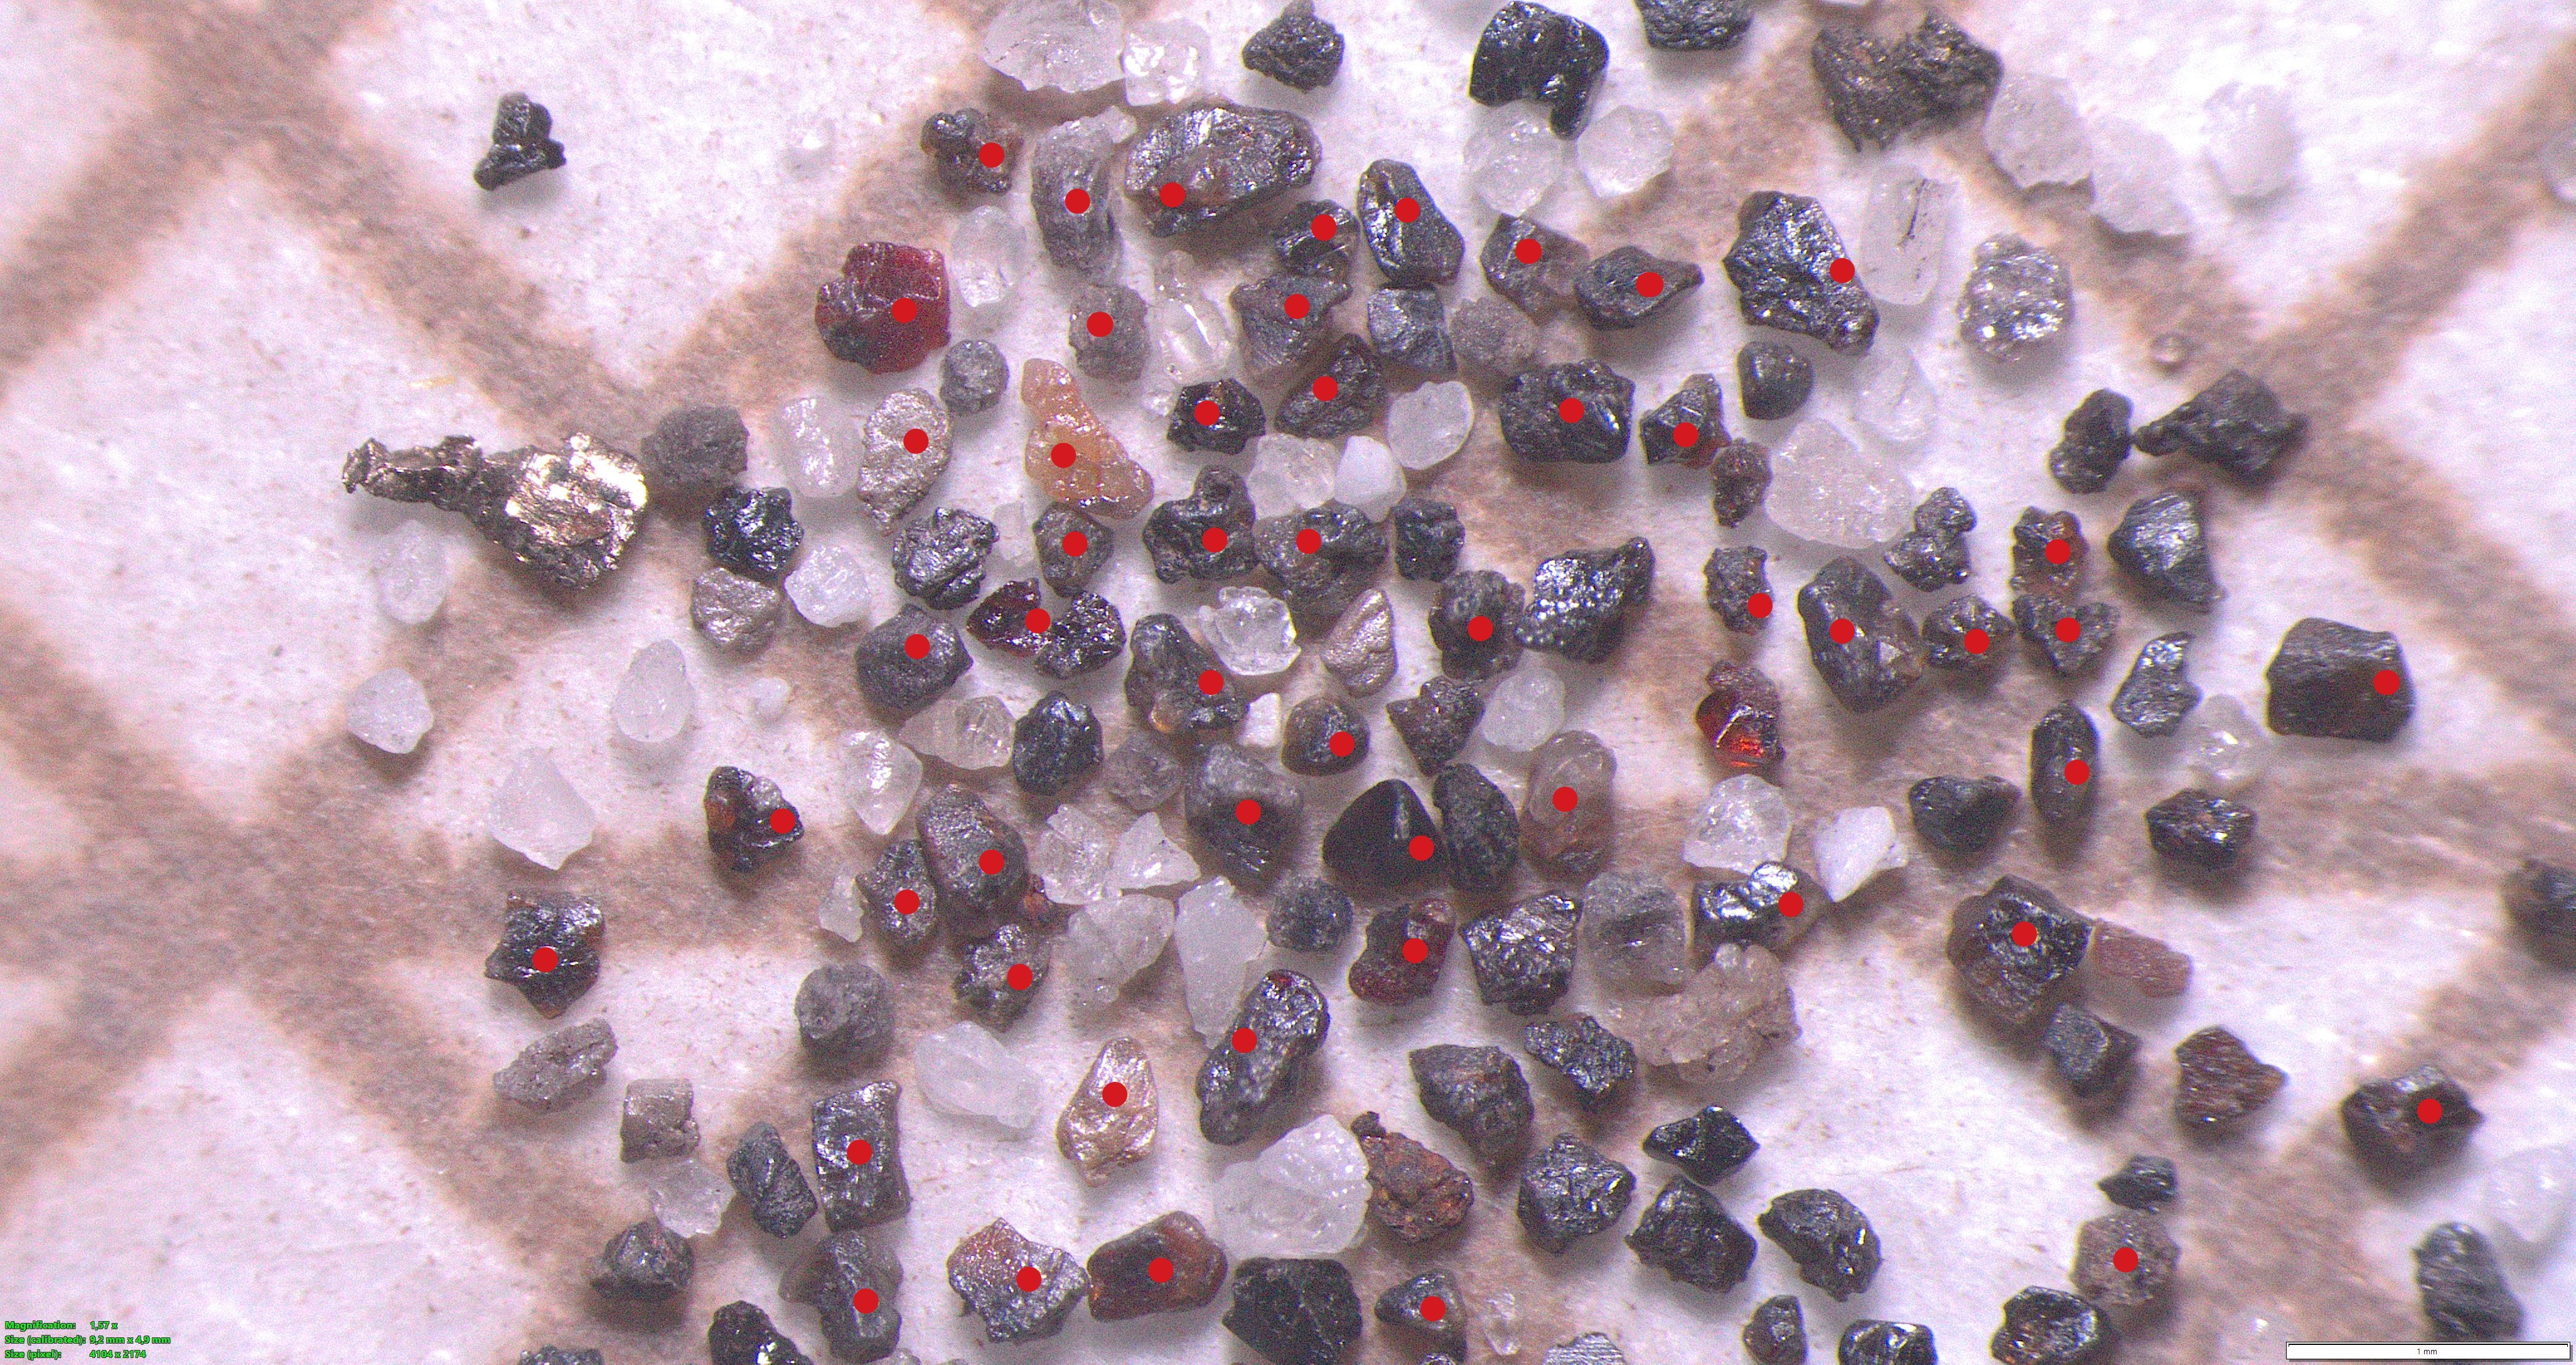
\includegraphics[width=\textwidth]{figure/anotasiAwal.jpg}
        \caption{Hasil Anotasi Awal yang di lakukan oleh \textit{Anotator}}
        \label{fig:3.AnotasiAwal}
    \end{subfigure}
    \hfill
    \begin{subfigure}[b]{0.475\textwidth}
        \centering
        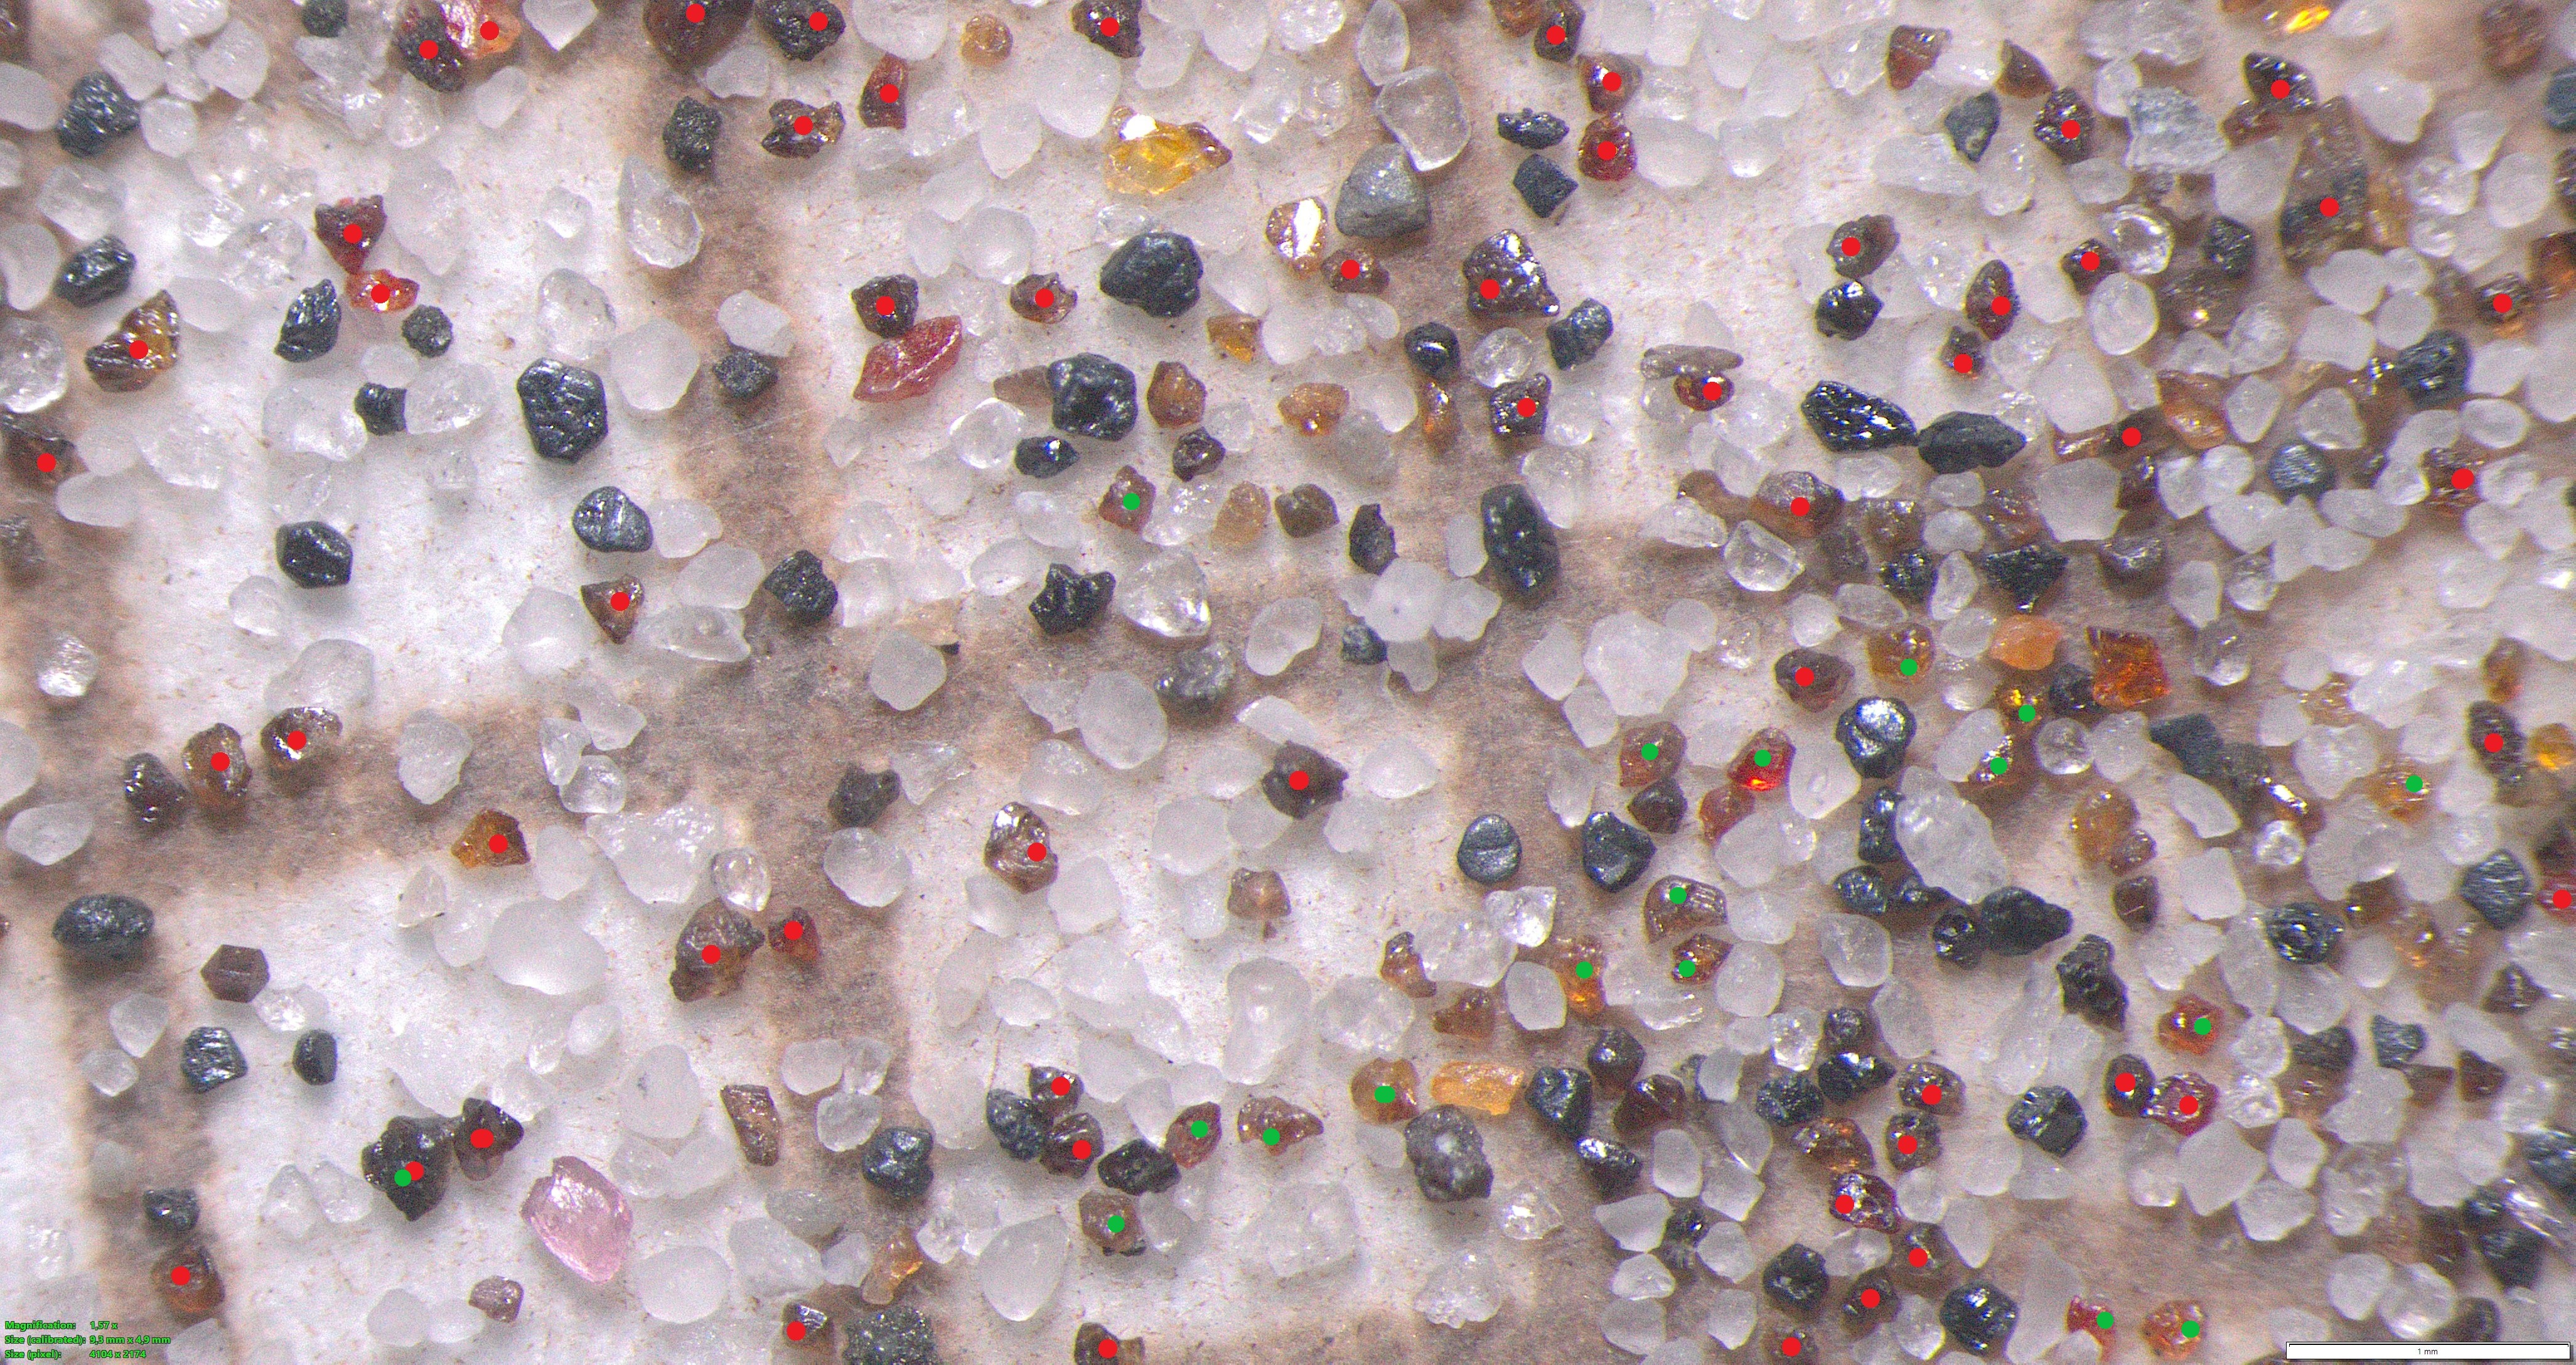
\includegraphics[width=\textwidth]{figure/AnotasiEval.jpg}
        \caption{Hasil Anotasi setelah di Evaluasi oleh \textit{Anotator}}
        \label{fig:3.AnotasiEval}
    \end{subfigure}

	\caption{Hasil Anotasi Data}
    \label{fig:3.HasilAnotasiData}
\end{figure}

\subsubsection{Segmentasi Data}
Pada tahap ini, dilakukan proses segmentasi data menggunakan LabelMe yang terintegrasi dengan \textit{Segment Anything} dengan fitur \textit{"Create Polygon with Segment Anything"}. Segmentasi dilakukan dengan metode poligon untuk mempermudah penandaan area kasiterit pada citra mikroskop. Dengan bantuan \textit{Segment Anything}, kontur mineral dapat diikuti secara otomatis, sehingga proses penandaan menjadi lebih efisien dan tetap fleksibel karena area mineral yang teroklusi dapat disesuaikan kembali secara manual dengan mengacu pada karakteristik bentuk kasiterit yang diperoleh dari wawancara pada tanggal 13 Agustus 2025 dengan Bapak Mesa Madestriasa selaku Kepala Laboratorium Eksplorasi PT. Timah Tbk., bahwa butiran kasiterit hasil preparasi umumnya berbentuk \textit{rounded} hingga \textit{sub-rounded} tanpa sudut angular, di mana tingkat kebulatanya semakin bulat pada butiran berukuran lebih kecil. Selain itu, penggunaan poligon yang dapat diedit membuat proses koreksi menjadi mudah dan tidak memerlukan langkah yang rumit. Labeling data dilakukan dalam satu kelas, setiap area yang ditandai diberi label yaitu \textit{"cassiterite"}. Dengan demikian, tahap ini memastikan bahwa data yang digunakan untuk pelatihan model segmentasi sudah teranotasi dan terlabel dengan baik. 

Dari keseluruhan proses segmentasi yang dilakukan terhadap 142 citra mikroskop, diperoleh total sebanyak 7,664 objek kasiterit yang berhasil diidentifikasi dan ditandai sebagai mask pada dataset. Jumlah ini merepresentasikan keseluruhan butiran kasiterit yang digunakan oleh model untuk mempelajari variasi bentuk, ukuran, serta karakteristik mineral pada tahap pelatihan. Contoh hasil segmentasi data ditunjukkan pada Gambar \ref{fig:3.HasilSegmentasiData} berikut. \par

\begin{figure}[H]
    \centering
    % Baris pertama: dua gambar sejajar
    \begin{subfigure}[b]{0.475\textwidth}
        \centering
        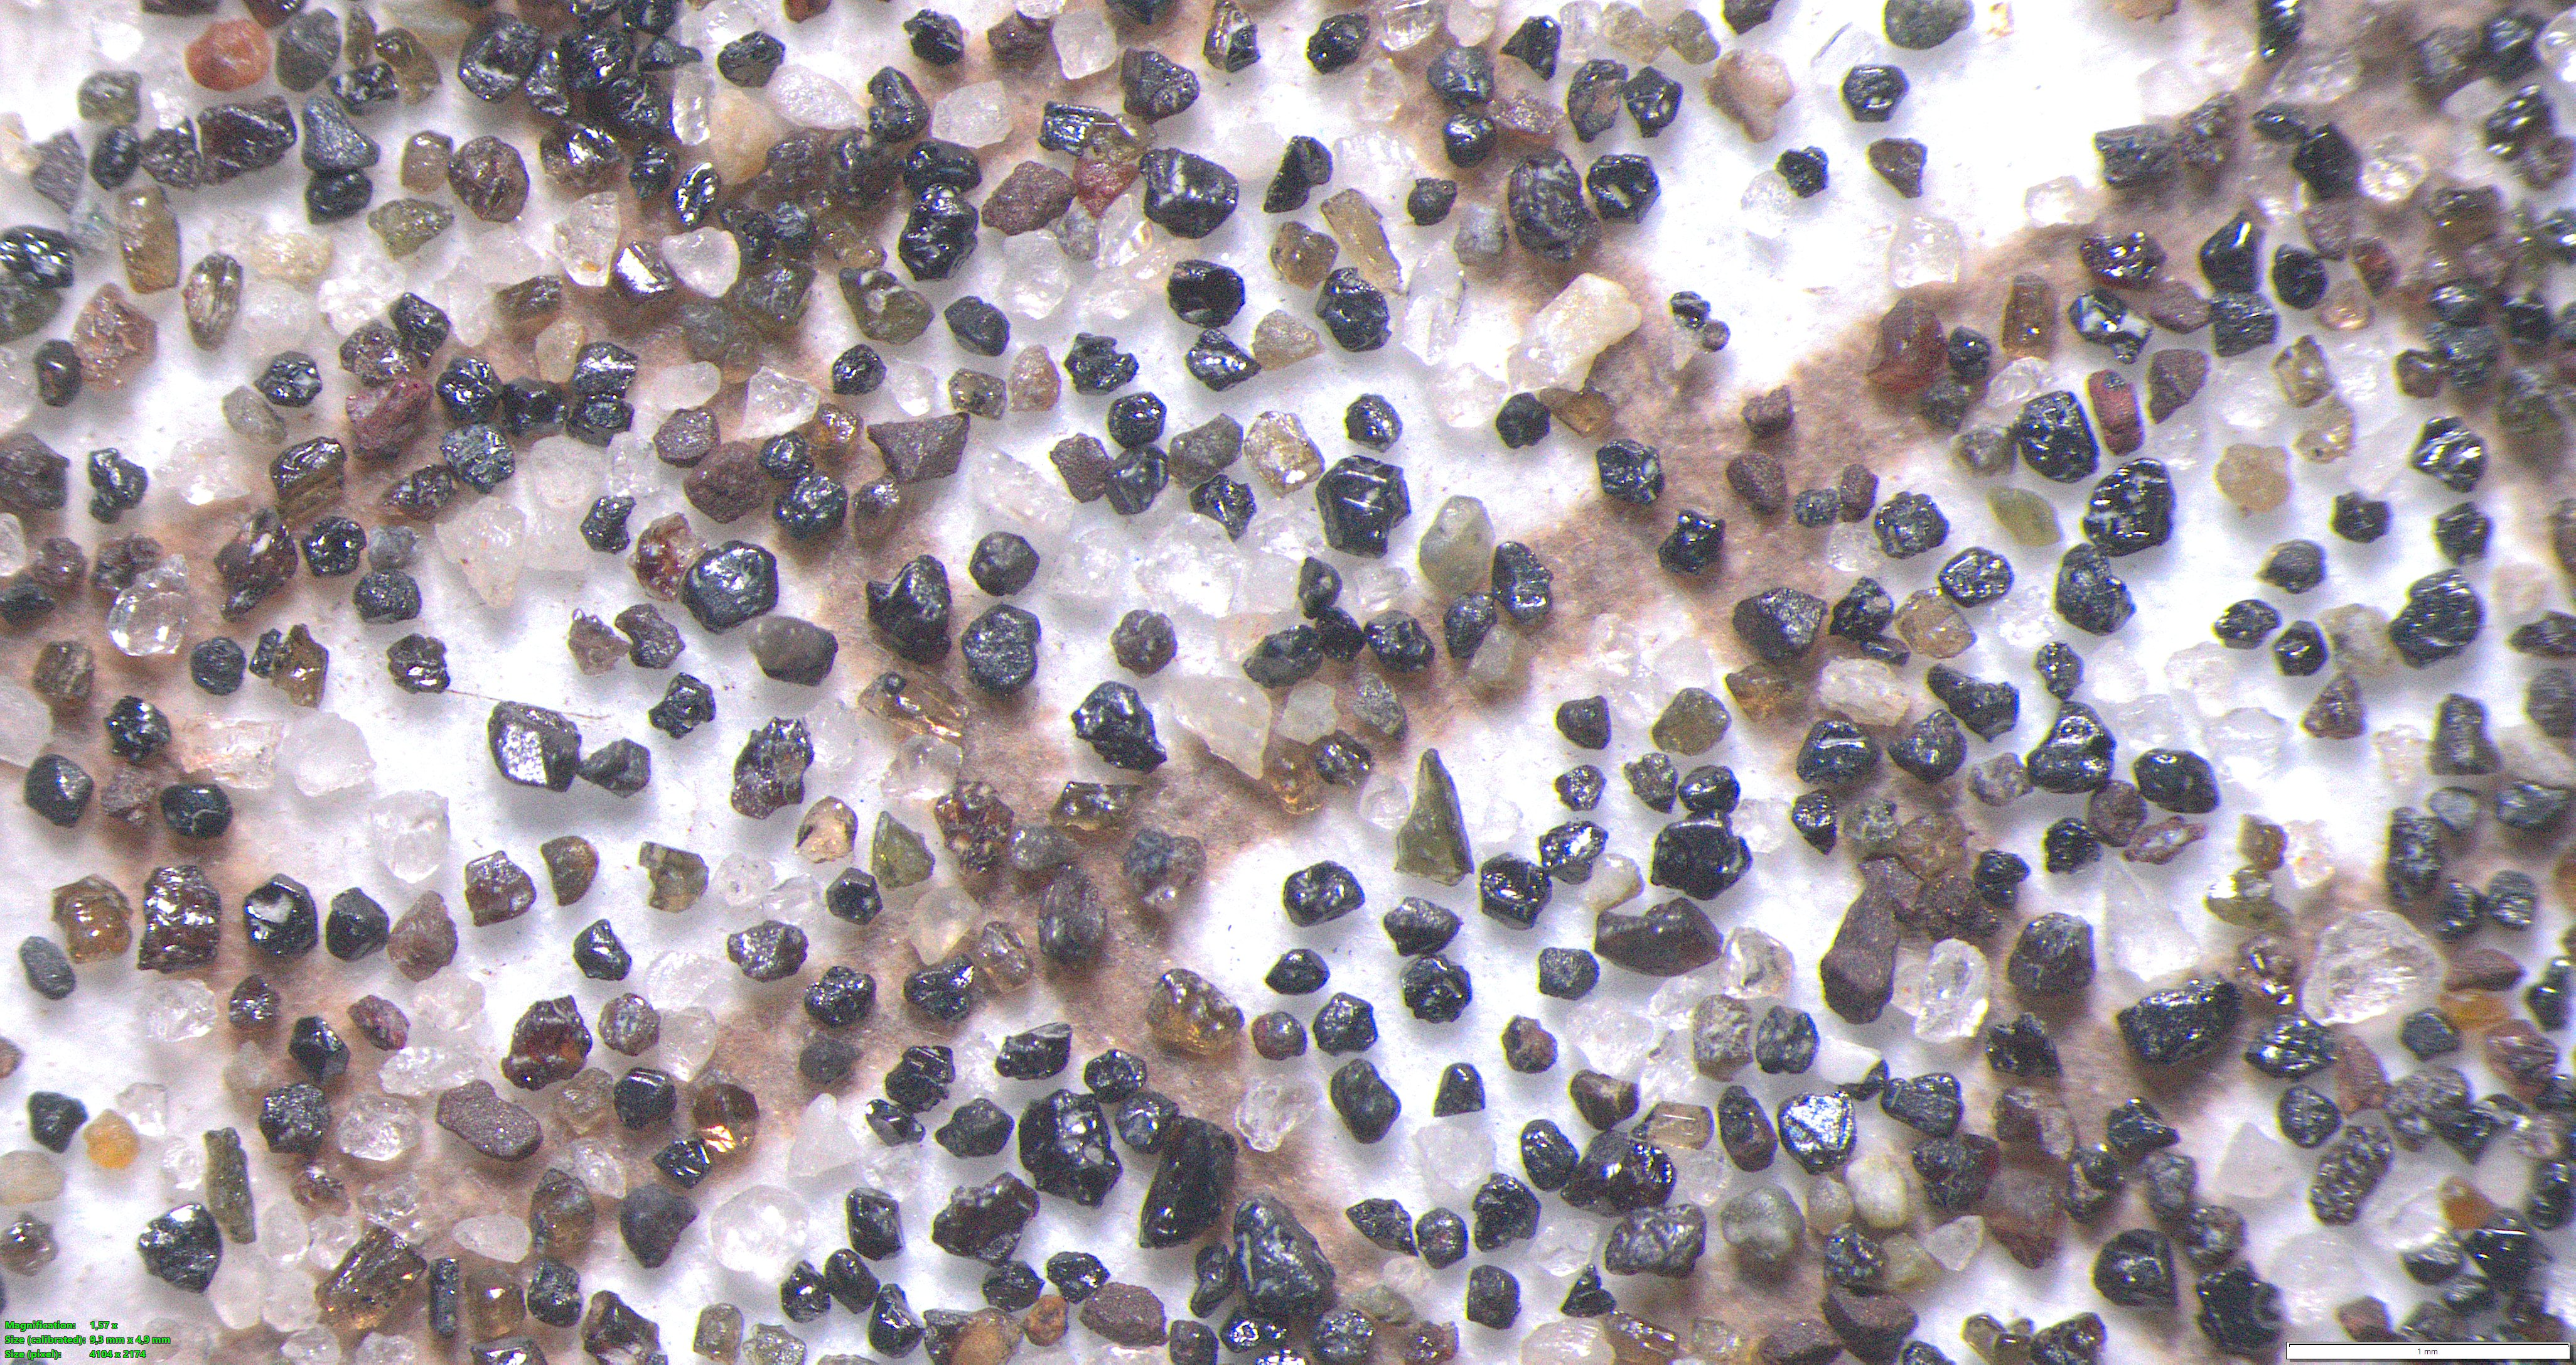
\includegraphics[width=\textwidth]{figure/input1.jpg}
        \caption{Data Sebelum Segmentasi}
        \label{fig:3.SebelumSegmentasi}
    \end{subfigure}
    \hfill
    \begin{subfigure}[b]{0.475\textwidth}
        \centering
        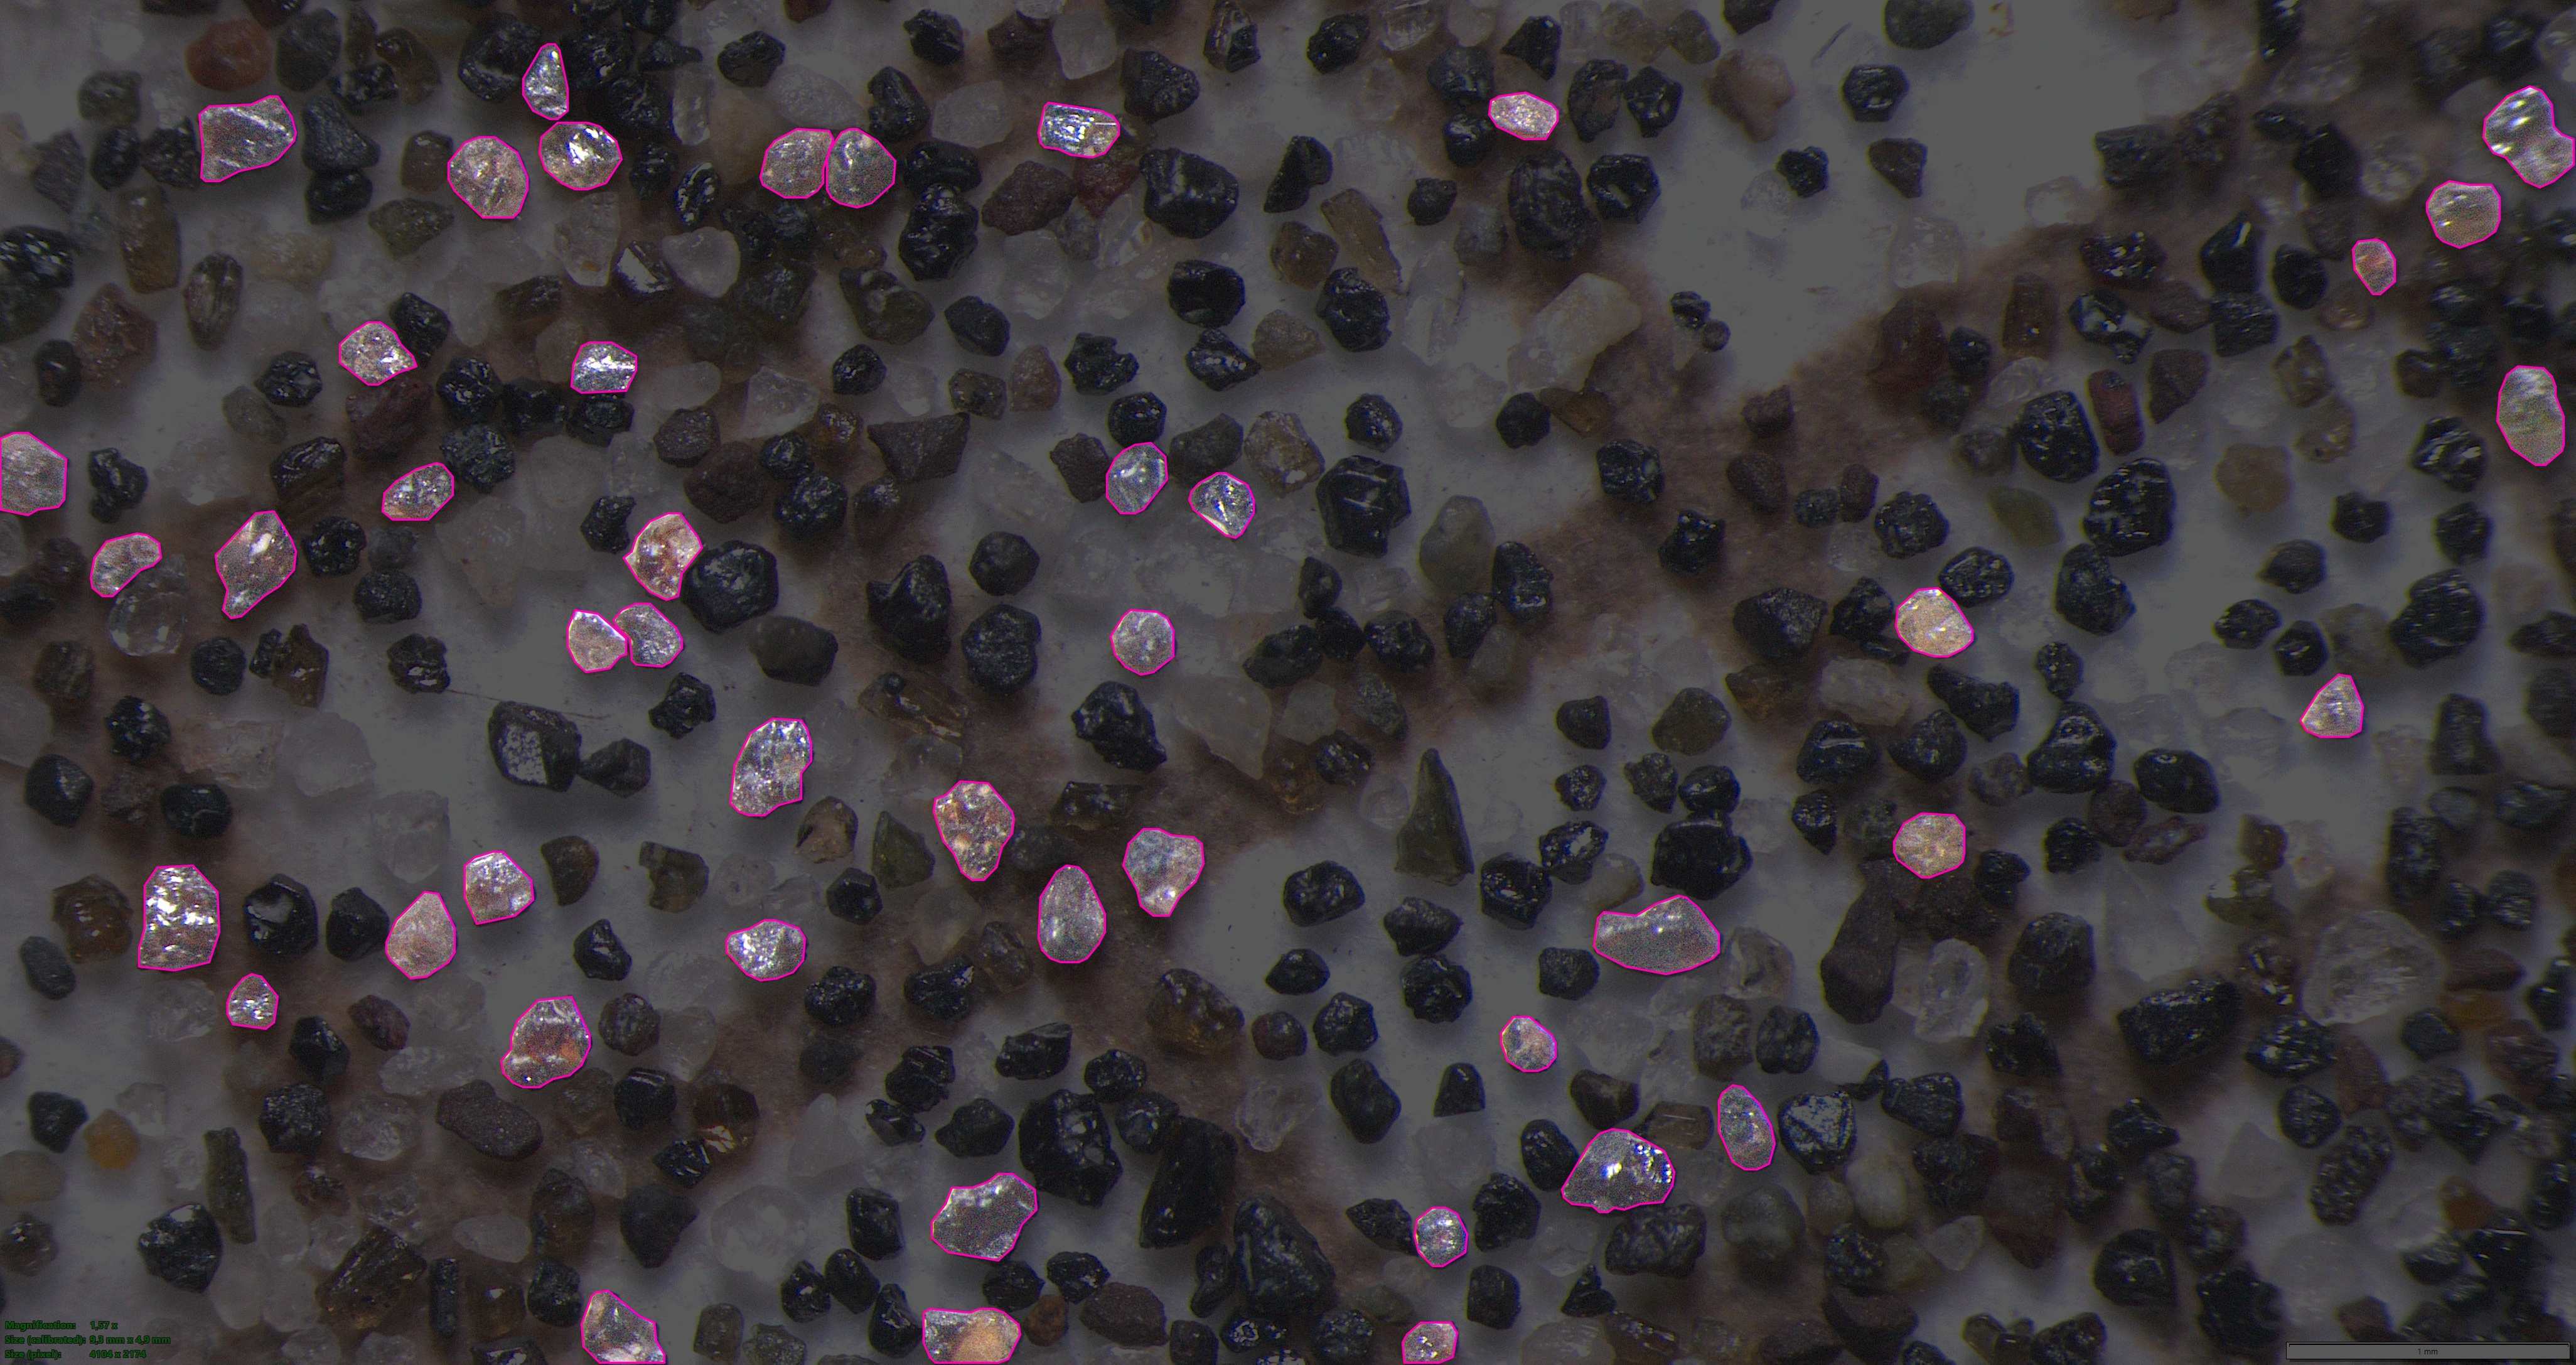
\includegraphics[width=\textwidth]{figure/output2.jpg}
        \caption{Data Setelah Segmentasi}
        \label{fig:3.SetelahSegmentasi}
    \end{subfigure}

	\caption{Hasil Segmentasi Data}
    \label{fig:3.HasilSegmentasiData}
\end{figure}

\subsubsection{Pembagian Citra (\textit{Image Tiling})} 
Pada tahap ini, dilakukan pembagian citra atau \textit{image tiling} untuk membagi citra beresolusi tinggi menjadi beberapa bagian yang lebih kecil atau \textit{patch}. Proses ini dilakukan sebagai alternatif dari proses \textit{resize} konvensional guna mempertahankan detail fitur pada butiran kasiterit yang berukuran kecil yang mungkin hilang jika resolusi citra dikurangi secara drastis. Dengan metode ini, model dapat mempelajari karakteristik objek pada resolusi aslinya tanpa melampaui kapasitas memori GPU. Citra asli dibagi menjadi grid $2 \times 2$, sehingga menghasilkan empat sub-citra yang lebih fokus. Contoh hasil pembagian citra ini ditunjukkan pada Gambar \ref{fig:3.HasilTilingData} berikut. \par

\begin{figure}[H]
    \centering
    % Baris pertama: satu gambar original di tengah
    \begin{subfigure}[b]{0.6\textwidth}
        \centering
        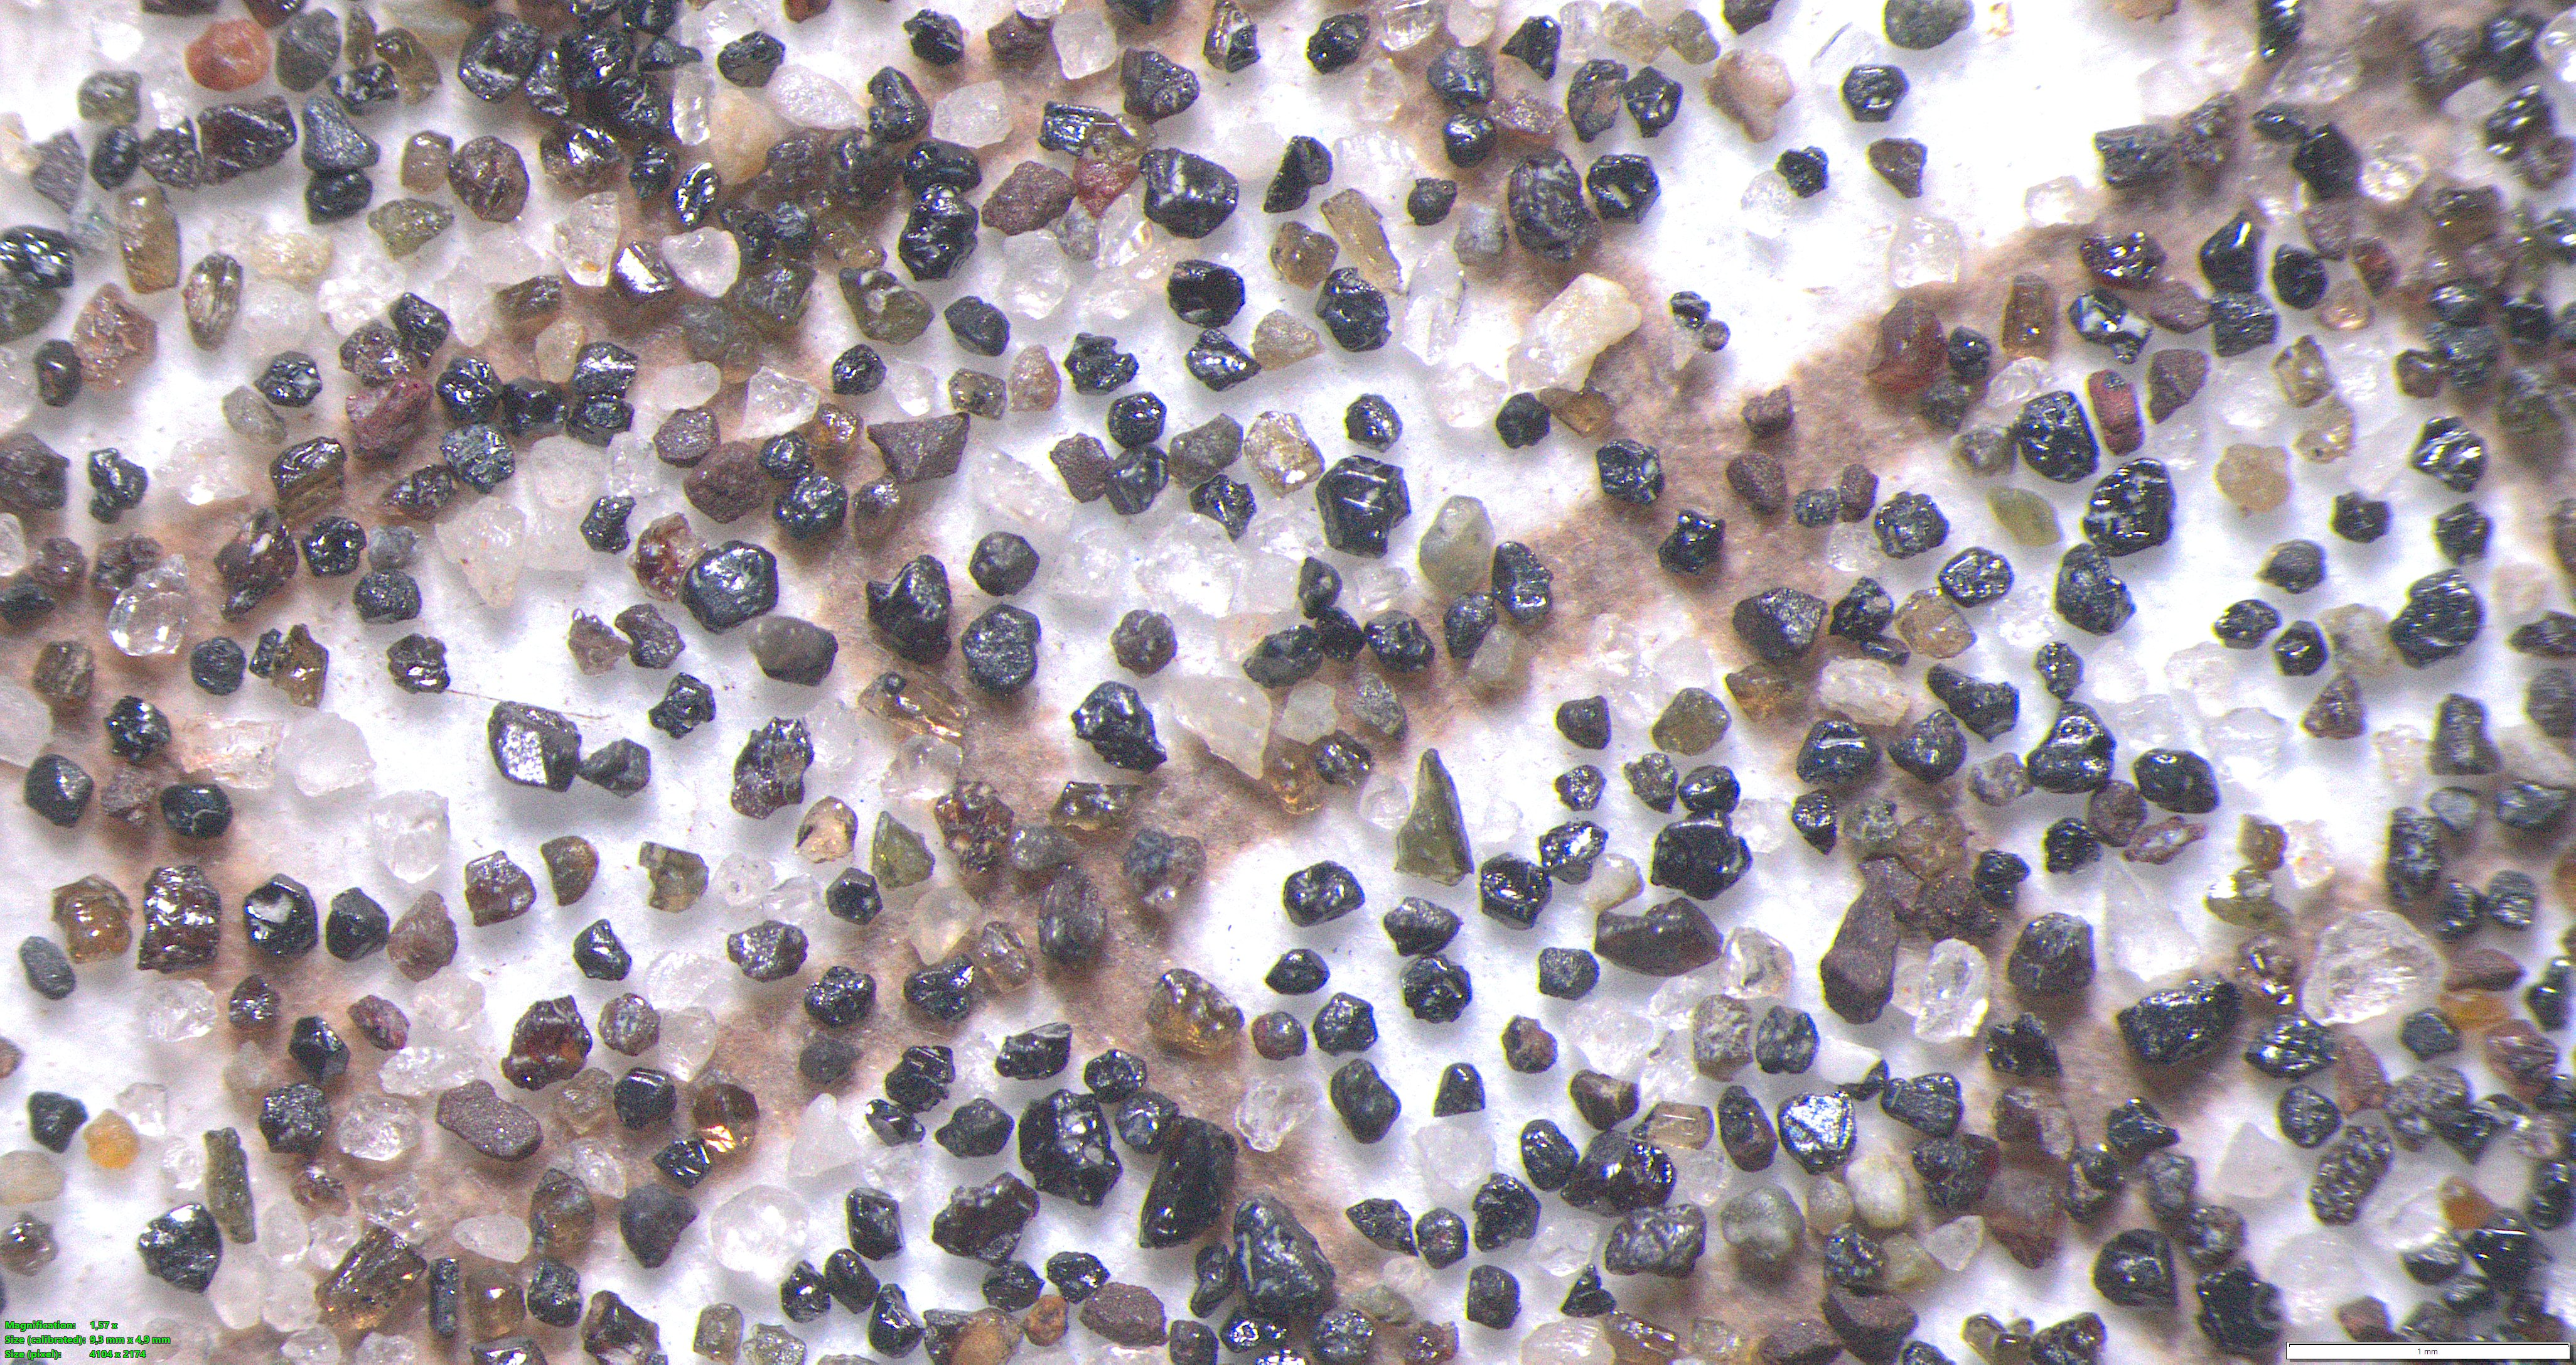
\includegraphics[width=\textwidth]{figure/tiles_285-25100F.jpg}
        \caption{Citra Original Sebelum \textit{Tiling}}
        \label{fig:3.TilingOriginal}
    \end{subfigure}
    
    \vskip\baselineskip
    
    % Baris kedua: grid 2x2 bagian atas
    \begin{subfigure}[b]{0.475\textwidth}
        \centering
        \includegraphics[width=\textwidth]{figure/285-25100F_tile0.png}
        \caption{Hasil \textit{Tiling} Bagian 1}
        \label{fig:3.Tile1}
    \end{subfigure}
    \hfill
    \begin{subfigure}[b]{0.475\textwidth}
        \centering
        \includegraphics[width=\textwidth]{figure/285-25100F_tile1.png}
        \caption{Hasil \textit{Tiling} Bagian 2}
        \label{fig:3.Tile2}
    \end{subfigure}
    
    \vskip\baselineskip
    
    % Baris ketiga: grid 2x2 bagian bawah
    \begin{subfigure}[b]{0.475\textwidth}
        \centering
        \includegraphics[width=\textwidth]{figure/285-25100F_tile2.png}
        \caption{Hasil \textit{Tiling} Bagian 3}
        \label{fig:3.Tile3}
    \end{subfigure}
    \hfill
    \begin{subfigure}[b]{0.475\textwidth}
        \centering
        \includegraphics[width=\textwidth]{figure/285-25100F_tile3.png}
        \caption{Hasil \textit{Tiling} Bagian 4}
        \label{fig:3.Tile4}
    \end{subfigure}

    \caption{Proses Pembagian Citra (\textit{Image Tiling}) Menjadi Grid $2 \times 2$}
    \label{fig:3.HasilTilingData}
\end{figure}

% % ini di bagi jadi 4 gambar
% \begin{figure}[H]
%     \centering
    
%     % Gambar original (tetap di atas, tengah)
%     \begin{subfigure}[b]{0.6\textwidth}
%         \centering
%         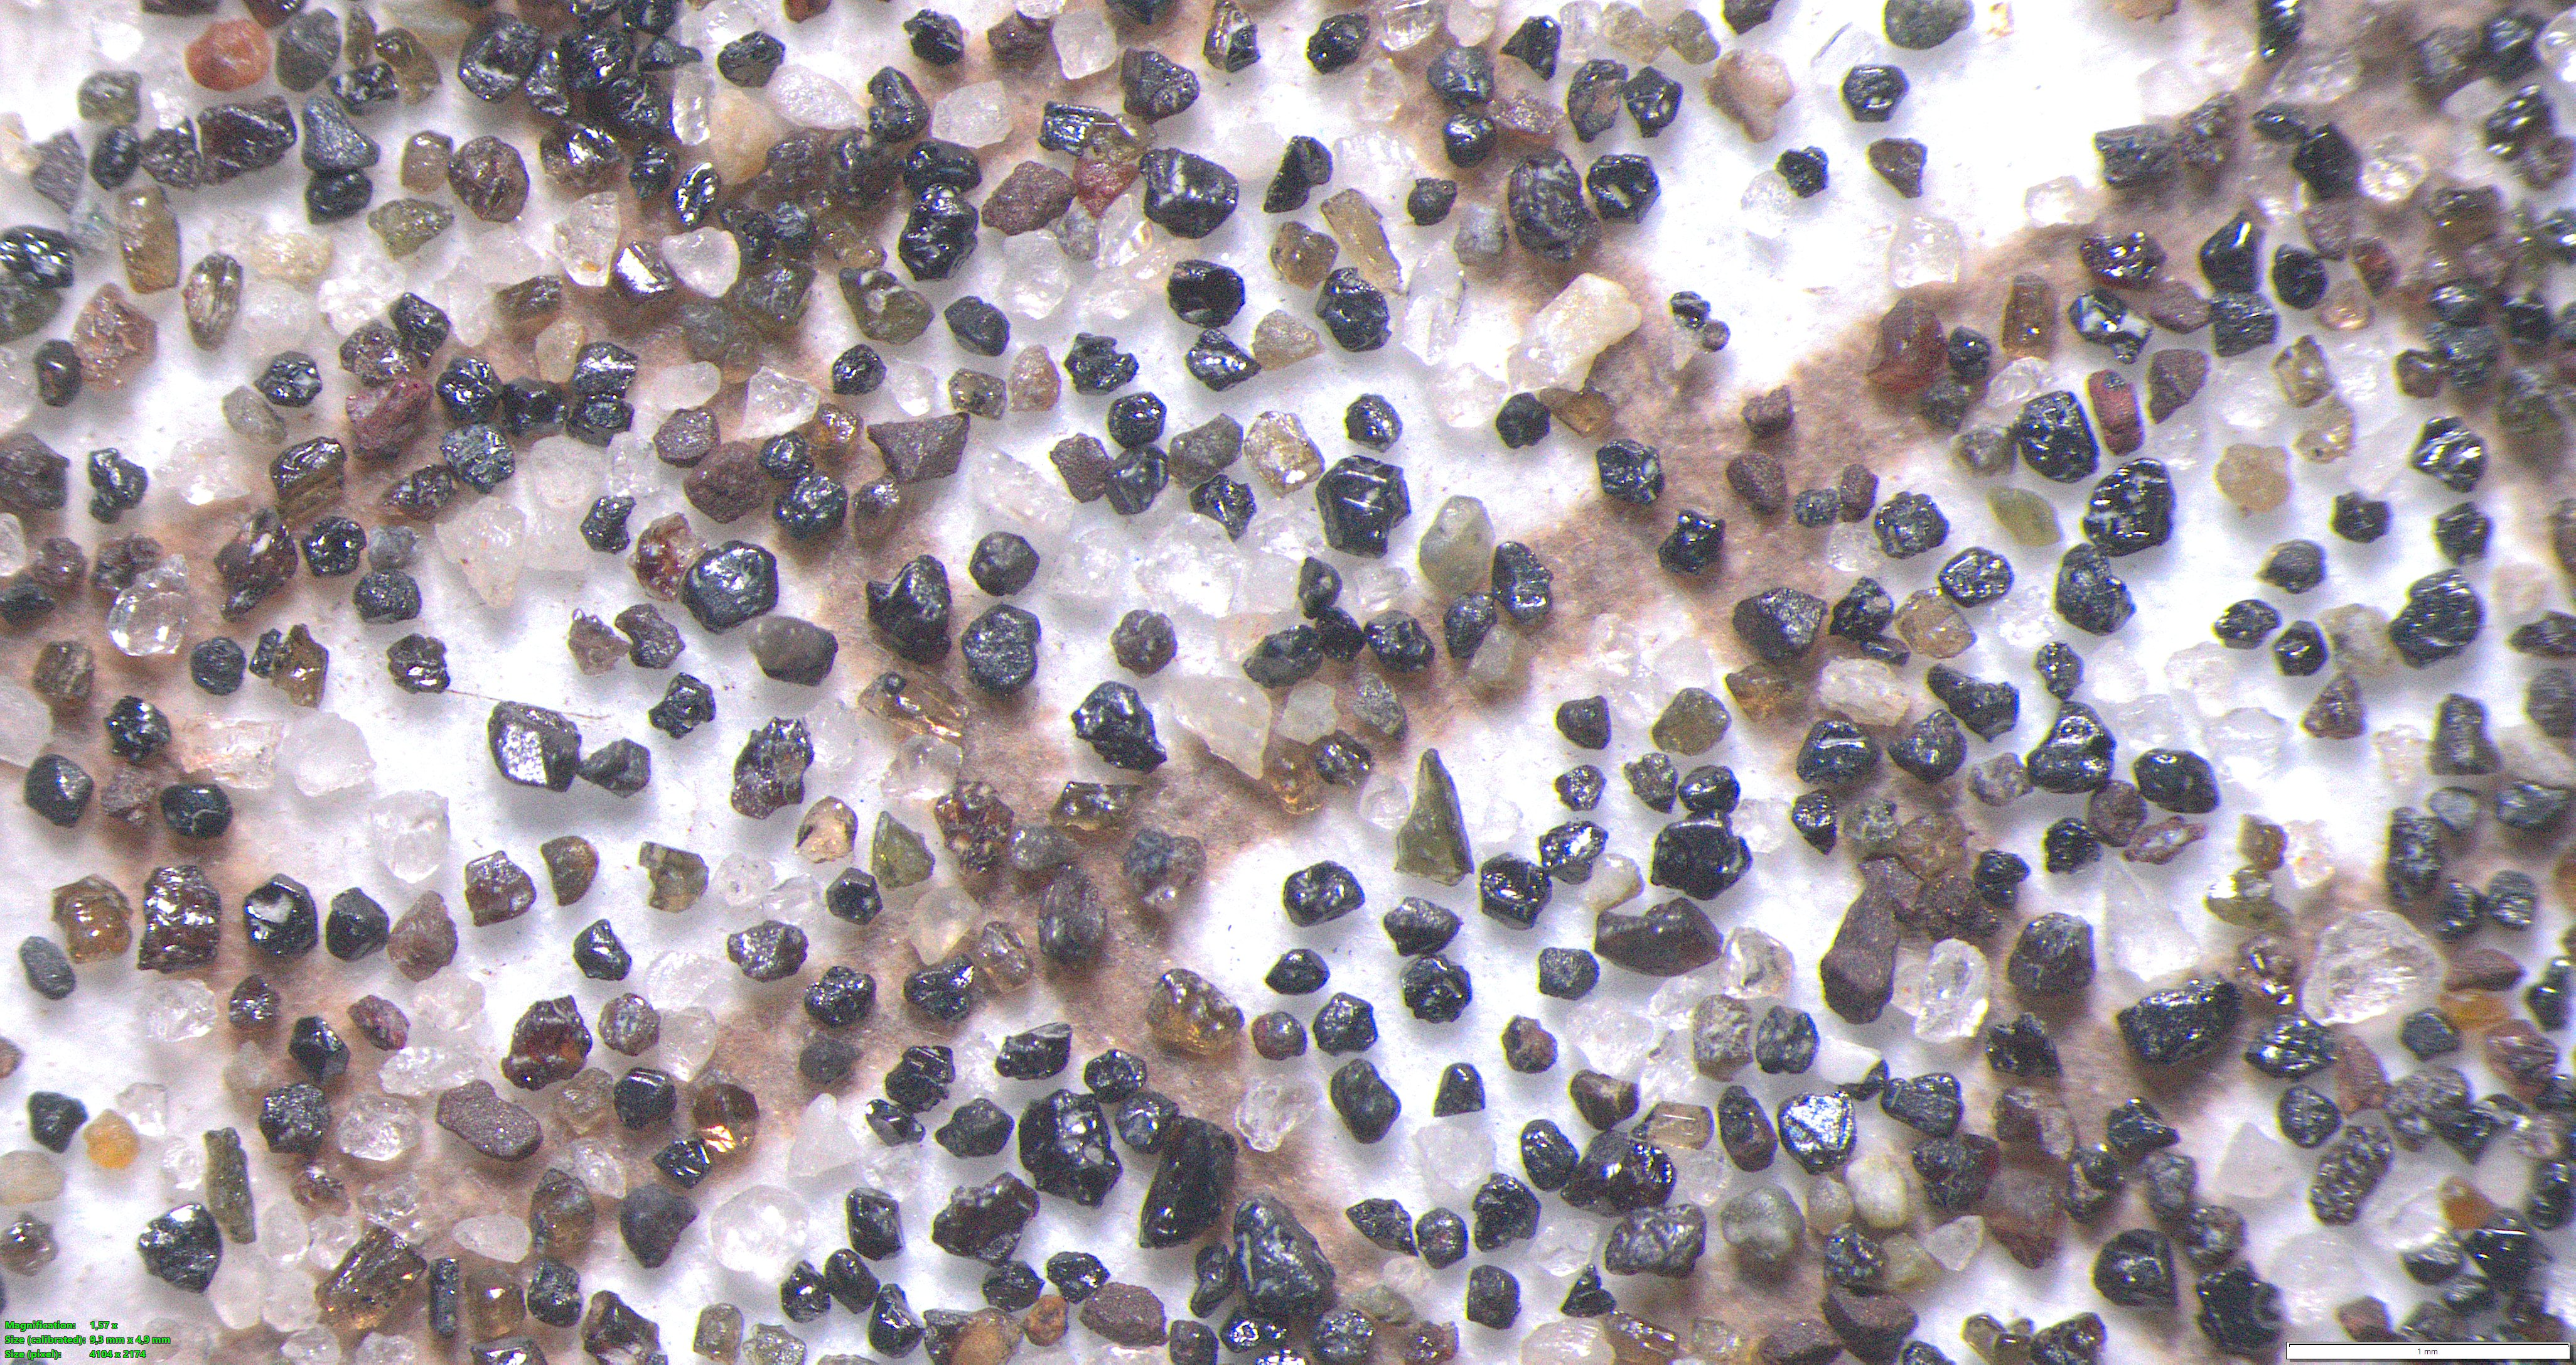
\includegraphics[width=\textwidth]{figure/tiles_285-25100F.jpg}
%         \caption{Citra Original Sebelum \textit{Tiling}}
%         \label{fig:3.TilingOriginal}
%     \end{subfigure}
    
%     \vskip\baselineskip
    
%     % 4 gambar sejajar satu baris
%     \begin{subfigure}[b]{0.24\textwidth}
%         \centering
%         \includegraphics[width=\textwidth]{figure/285-25100F_tile0.png}
%         \caption{Bagian 1}
%         \label{fig:3.Tile1}
%     \end{subfigure}
%     \hfill
%     \begin{subfigure}[b]{0.24\textwidth}
%         \centering
%         \includegraphics[width=\textwidth]{figure/285-25100F_tile1.png}
%         \caption{Bagian 2}
%         \label{fig:3.Tile2}
%     \end{subfigure}
%     \hfill
%     \begin{subfigure}[b]{0.24\textwidth}
%         \centering
%         \includegraphics[width=\textwidth]{figure/285-25100F_tile2.png}
%         \caption{Bagian 3}
%         \label{fig:3.Tile3}
%     \end{subfigure}
%     \hfill
%     \begin{subfigure}[b]{0.24\textwidth}
%         \centering
%         \includegraphics[width=\textwidth]{figure/285-25100F_tile3.png}
%         \caption{Bagian 4}
%         \label{fig:3.Tile4}
%     \end{subfigure}

%     \caption{Proses Pembagian Citra (\textit{Image Tiling}) Menjadi Grid $2 \times 2$}
%     \label{fig:3.HasilTilingData}
% \end{figure}


% \subsubsection{\textit{Resize}}
% Pada tahapan ini, data diproses untuk menghasilkan kumpulan data dengan ukuran yang seragam, yaitu  $1920 \times 1080$ piksel. Ukuran data dipilih berdasarkan resolusi asli citra mikroskop yang diperoleh dari Laboratorium Eksplorasi PT. Timah Tbk., yakni terdapat dua ukuran yaitu $1920 \times 1080$ piksel dan $4104 \times 2174$ piksel. Penyeragaman ukuran citra dilakukan agar seluruh data memiliki dimensi yang konsisten, sehingga memudahkan proses pelatihan model dan menghindari ketidaksesuaian resolusi yang dapat memengaruhi hasil segmentasi. Selain itu, pemilihan ukuran $1920 \times 1080$ piksel juga dipertimbangkan untuk menjaga keseimbangan antara kualitas detail citra dan efisiensi komputasi selama proses pemrosesan data. Contoh hasil perubahan resolusi citra dari ukuran awal menjadi ukuran seragam ditunjukkan pada Gambar \ref{fig:3.HasilResizeData} berikut. \par

% \begin{figure}[H]
%     \centering
%     % Baris pertama: dua gambar sejajar
%     \begin{subfigure}[b]{0.475\textwidth}
%         \centering
%         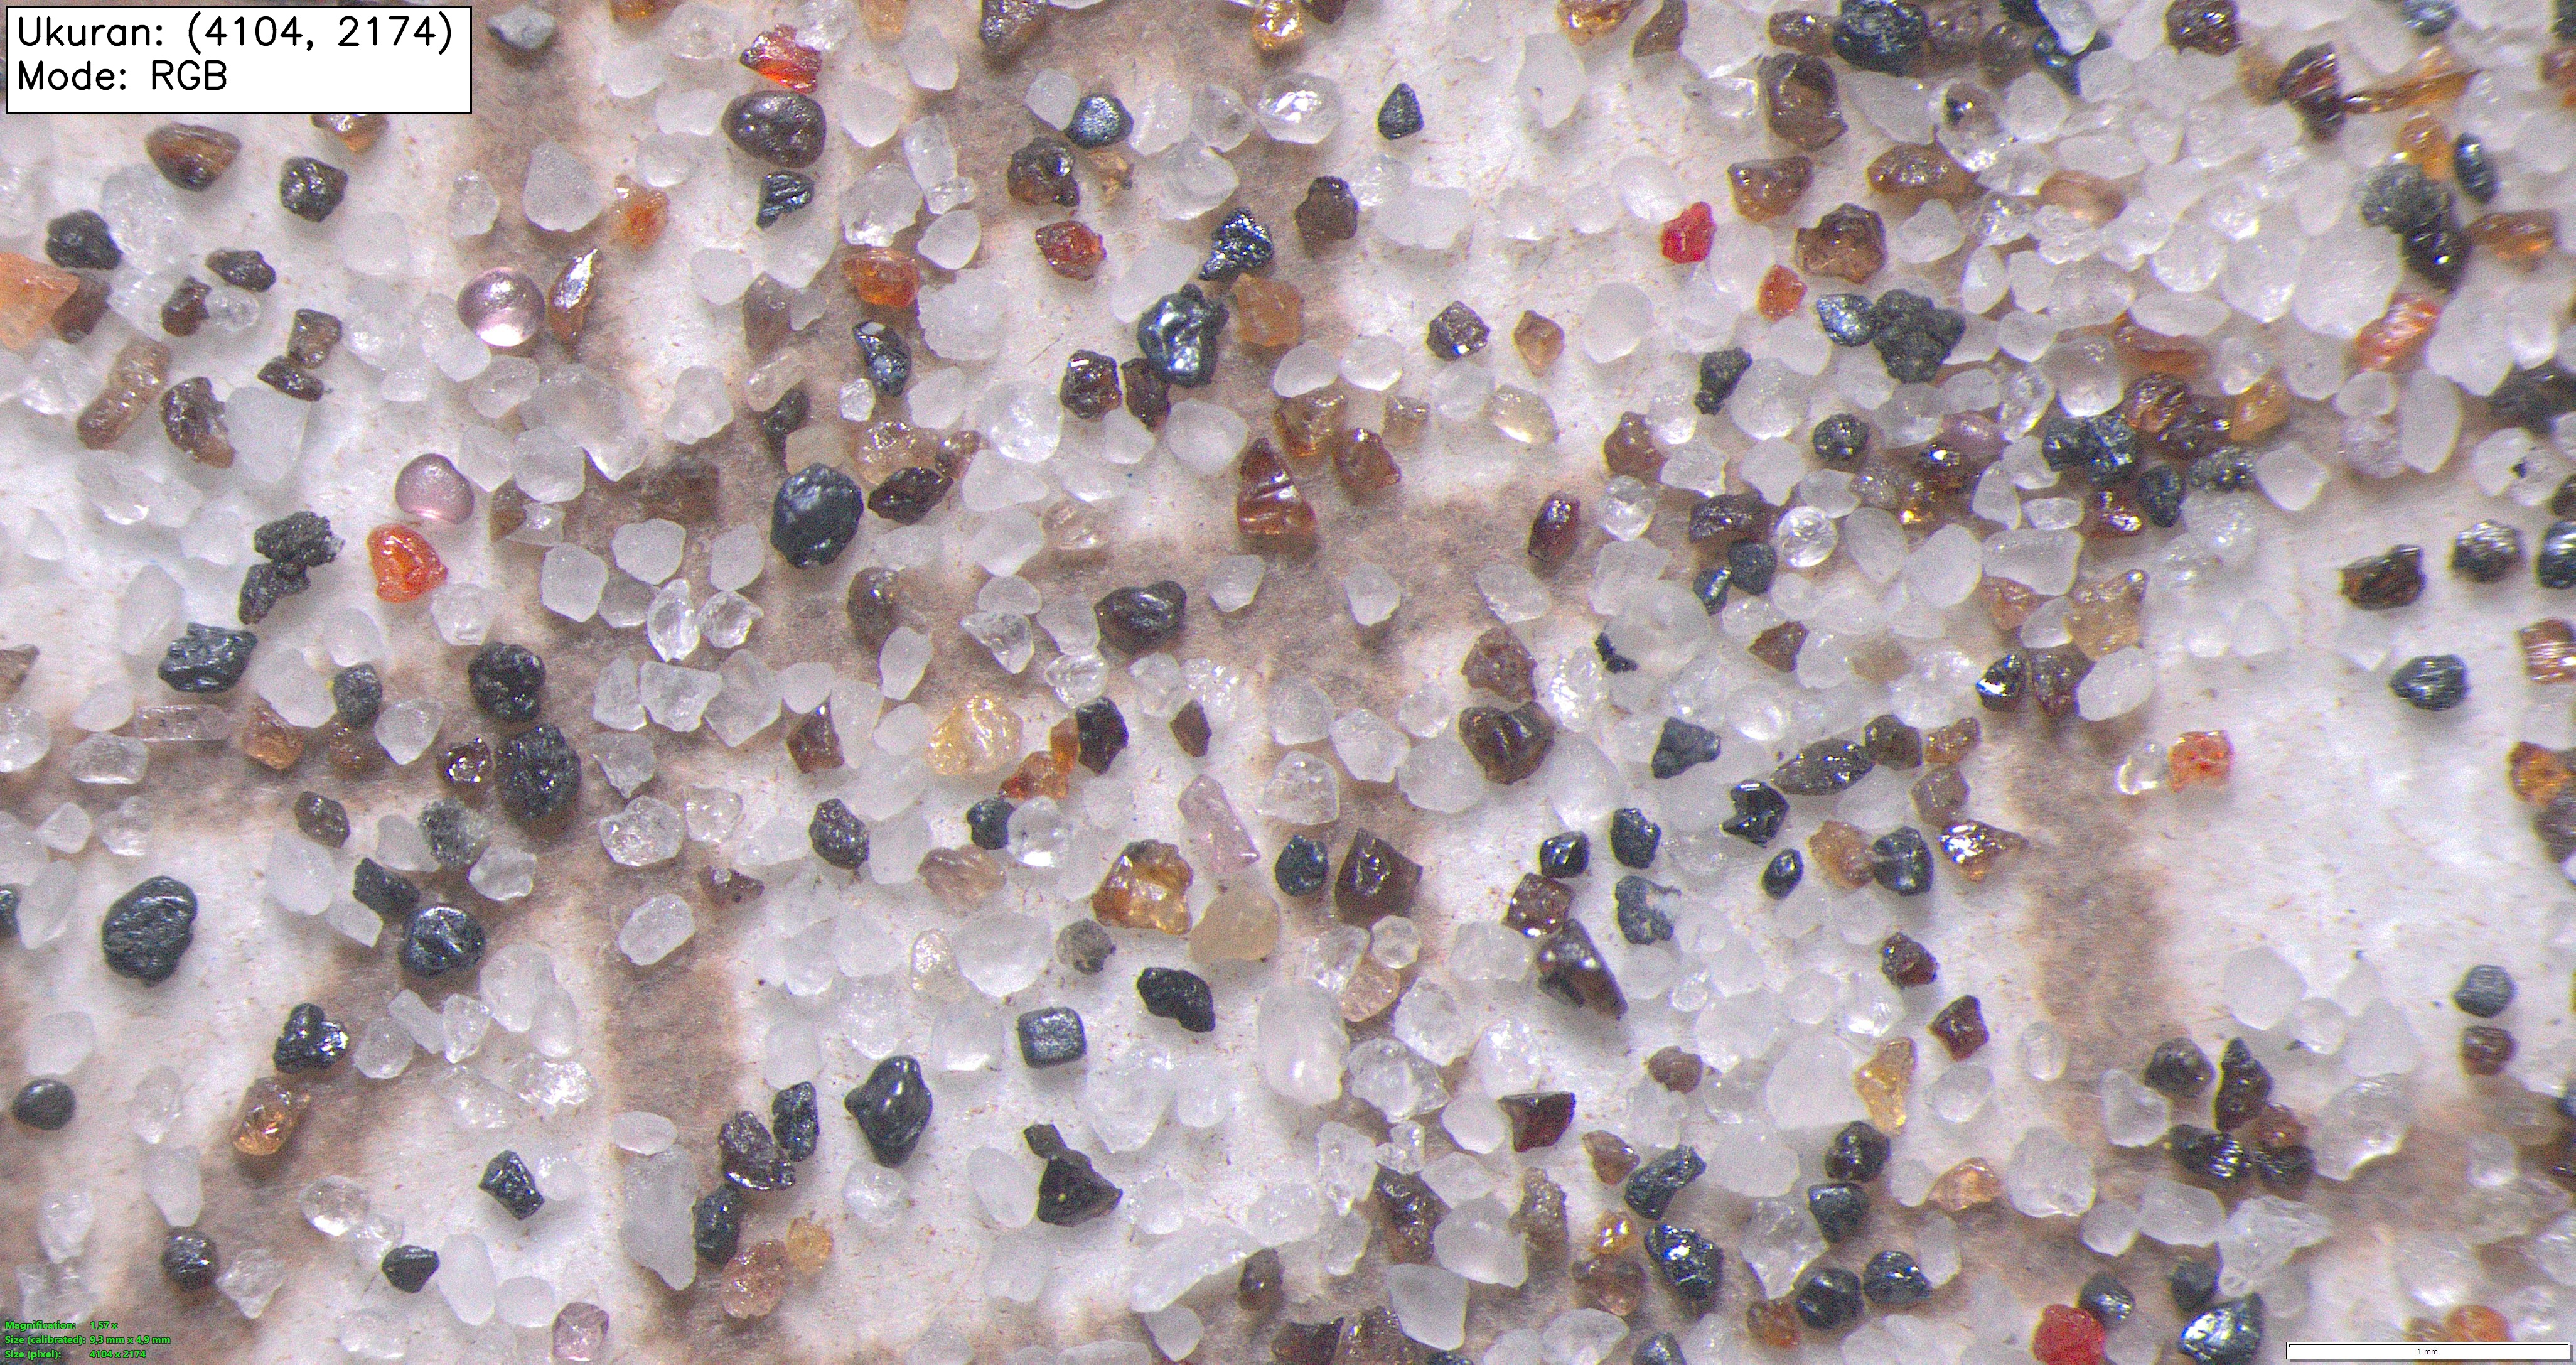
\includegraphics[width=\textwidth]{figure/hasilResizeAsli_denganKeterangan.jpg}
%         \caption{Citra Awal dengan resolusi $4104 \times 2174$ piksel}
%         \label{fig:3.ResizeAwal}
%     \end{subfigure}
%     \hfill
%     \begin{subfigure}[b]{0.475\textwidth}
%         \centering
%         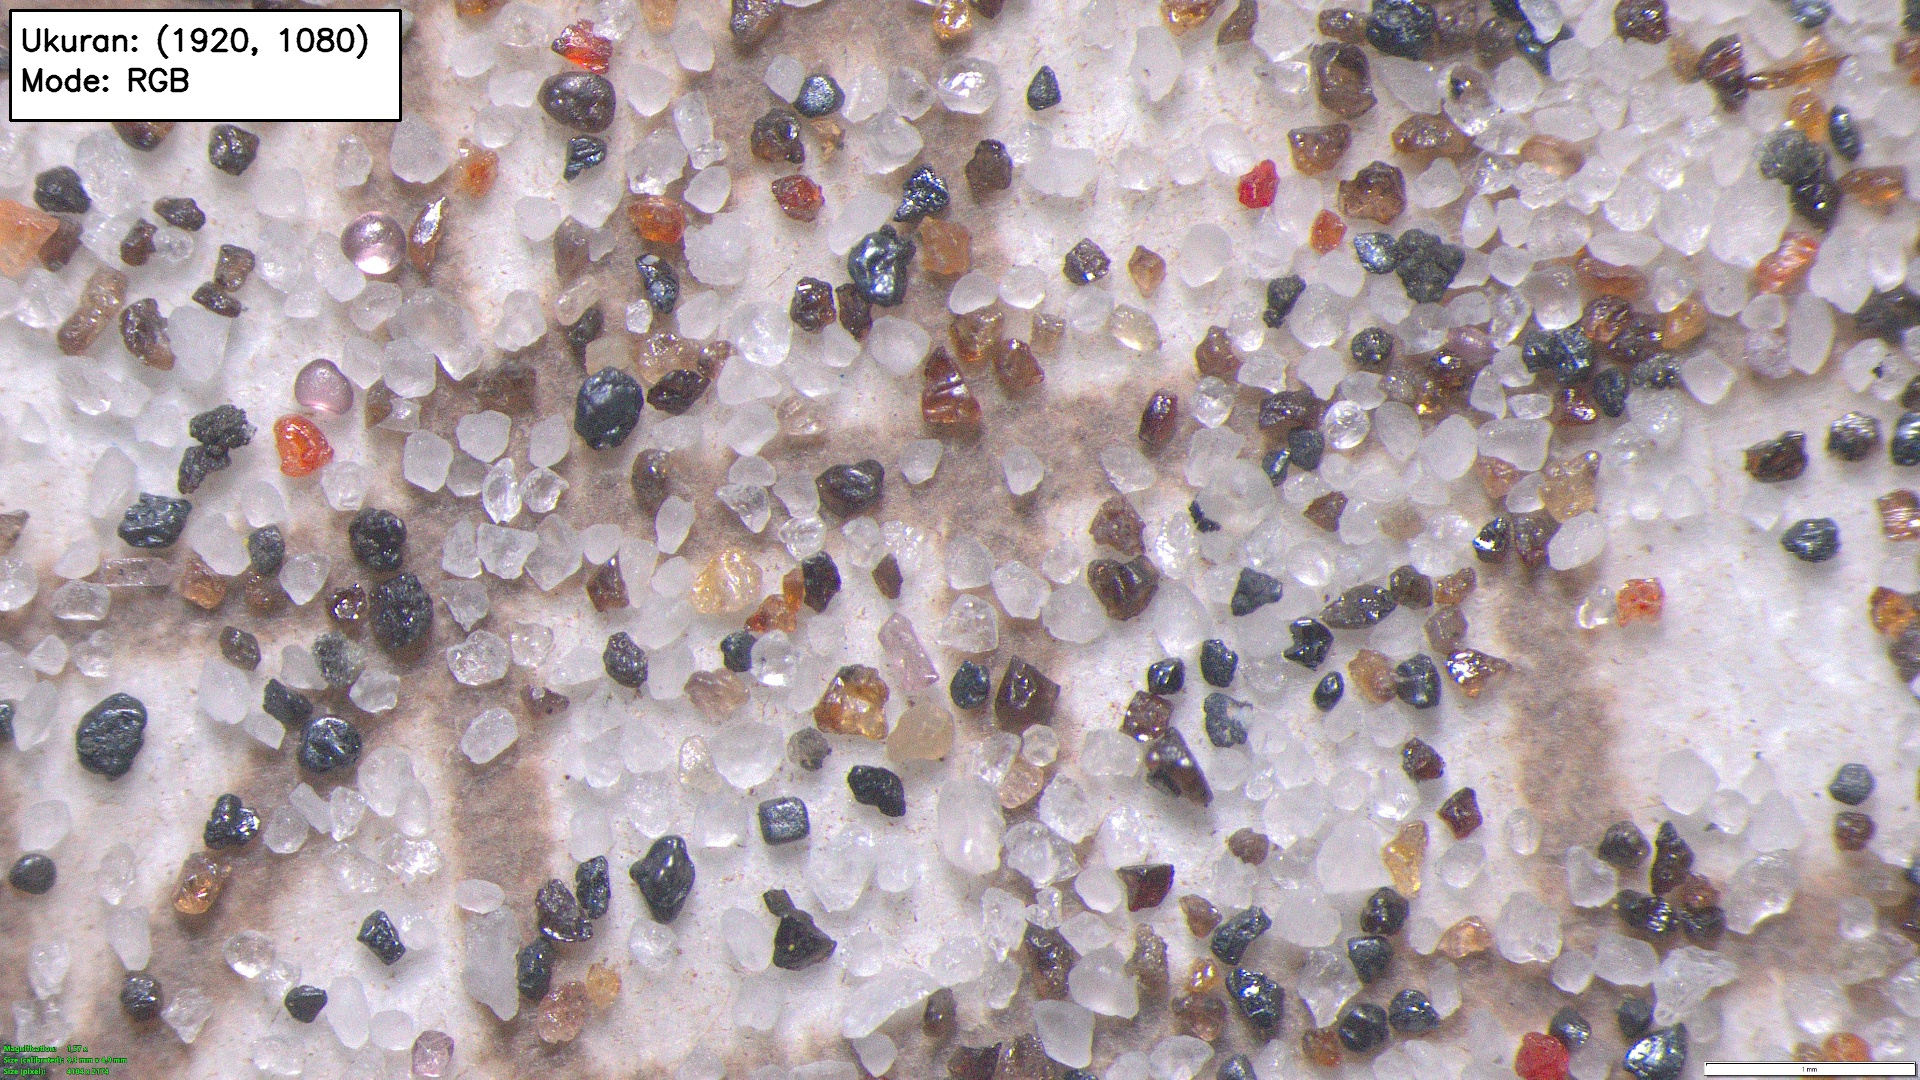
\includegraphics[width=\textwidth]{figure/hasilResize_denganKeterangan.jpg}
%         \caption{Hasil Resize dengan resolusi $1920 \times 1080$ piksel}
%         \label{fig:3.ResizeAkhir}
%     \end{subfigure}

% 	\caption{Hasil Resize Data}
%     \label{fig:3.HasilResizeData}
% \end{figure}

\subsubsection{Augmentasi Data}
Augmentasi yang dilakukan pada penelitian ini meliputi teknik \textit{flip}, \textit{rotate}, dan penambahan \textit{Gaussian noise}. Teknik-teknik ini diterapkan untuk memperkaya variasi data pelatihan, sehingga model dapat belajar mengenali objek mineral kasiterit dalam berbagai kondisi visual yang berbeda. Berikut merupakan penjelasan dari masing-masing teknik augmentasi yang diterapkan.\par

\subsubsection*{\textnormal{1. \textit{Flip}}}
Pada tahapan ini, data citra mikroskop diolah dengan menerapkan teknik augmentasi \textit{flip} yang membalik citra baik secara \textit{horizontal} maupun \textit{vertikal} untuk menambah variasi data pelatihan \cite{thesisNova}. Teknik ini digunakan agar model dapat mengenali objek mineral kasiterit dari berbagai orientasi tanpa kehilangan informasi penting pada citra. Dengan adanya \textit{HorizontalFlip} dan \textit{VerticalFlip} yang diterapkan secara acak, model menjadi lebih \textit{robust} terhadap perubahan posisi atau arah objek pada citra mikroskop. Contoh hasil penerapan teknik \textit{flip} secara \textit{horizontal} dan \textit{vertikal} ditunjukkan pada Gambar \ref{fig:3.HasilFlipData} berikut.\par

\begin{figure}[H]
    \centering
    % Baris pertama: dua gambar sejajar
    \begin{subfigure}[b]{0.475\textwidth}
        \centering
        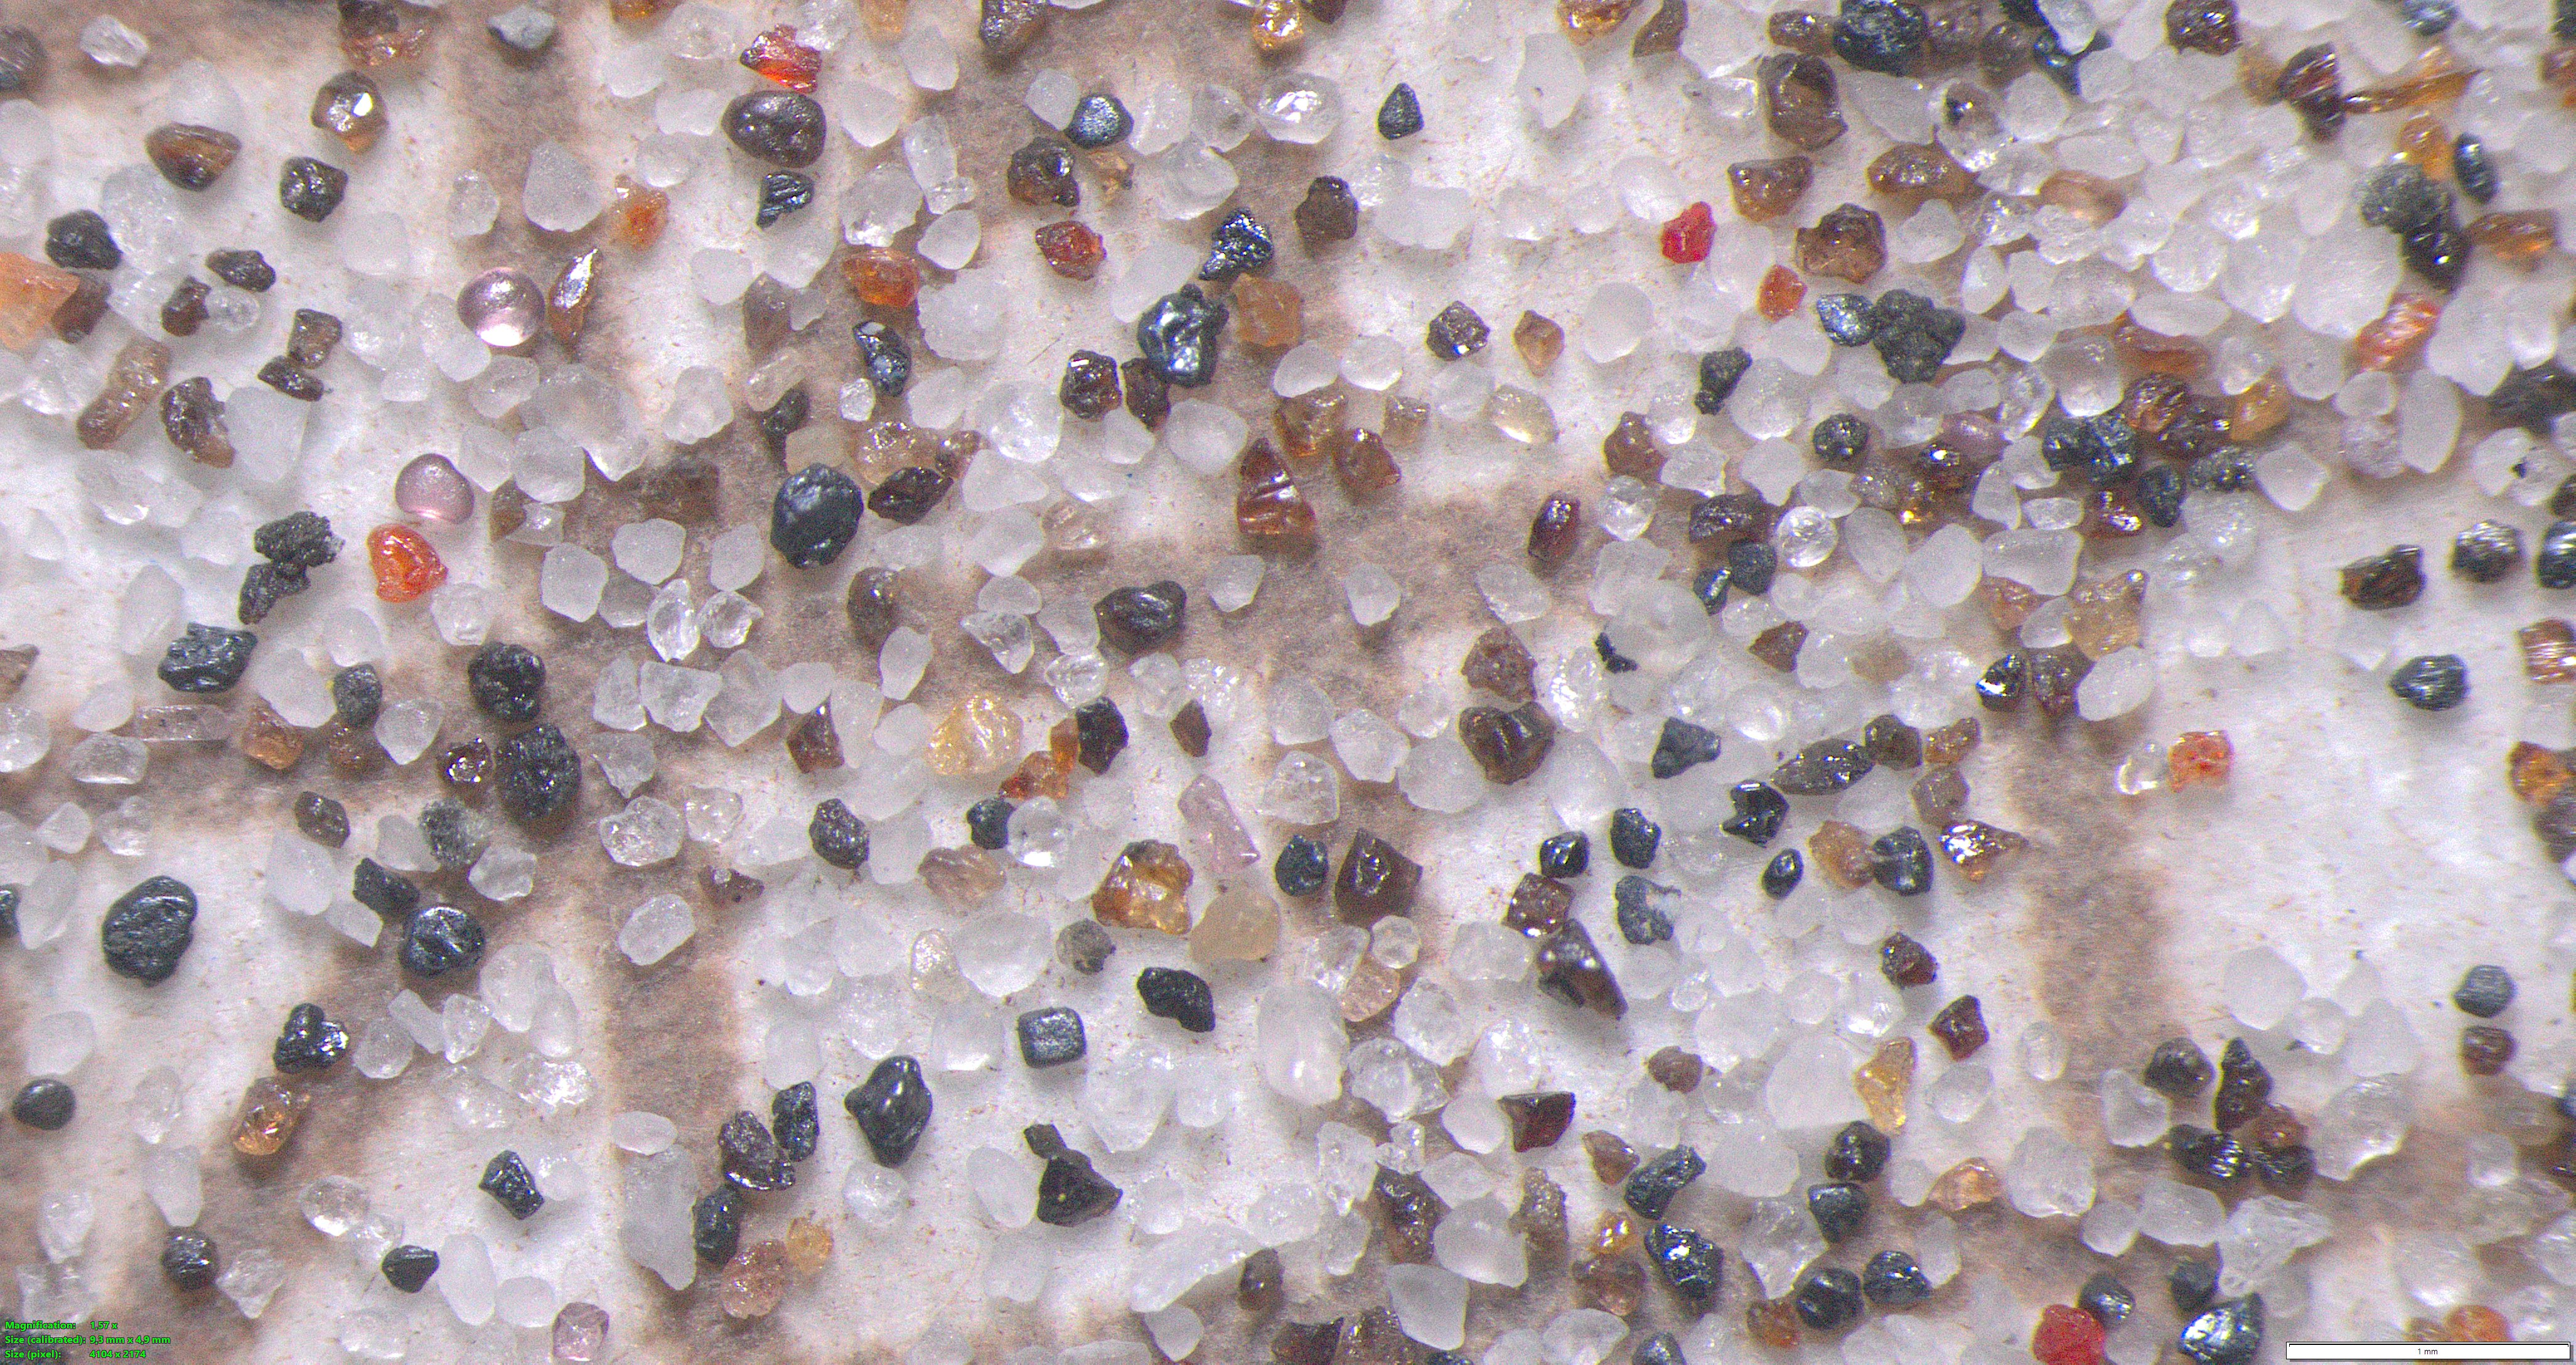
\includegraphics[width=\textwidth]{figure/sebeleumResize.jpg}
        \caption{Citra Awal tanpa \textit{Flip}}
        \label{fig:3.CitraAwalFlip}
    \end{subfigure}
    
    % Baris kedua: satu gambar di bawah tengah
    \vskip\baselineskip
    \begin{subfigure}[b]{0.475\textwidth}
        \centering
        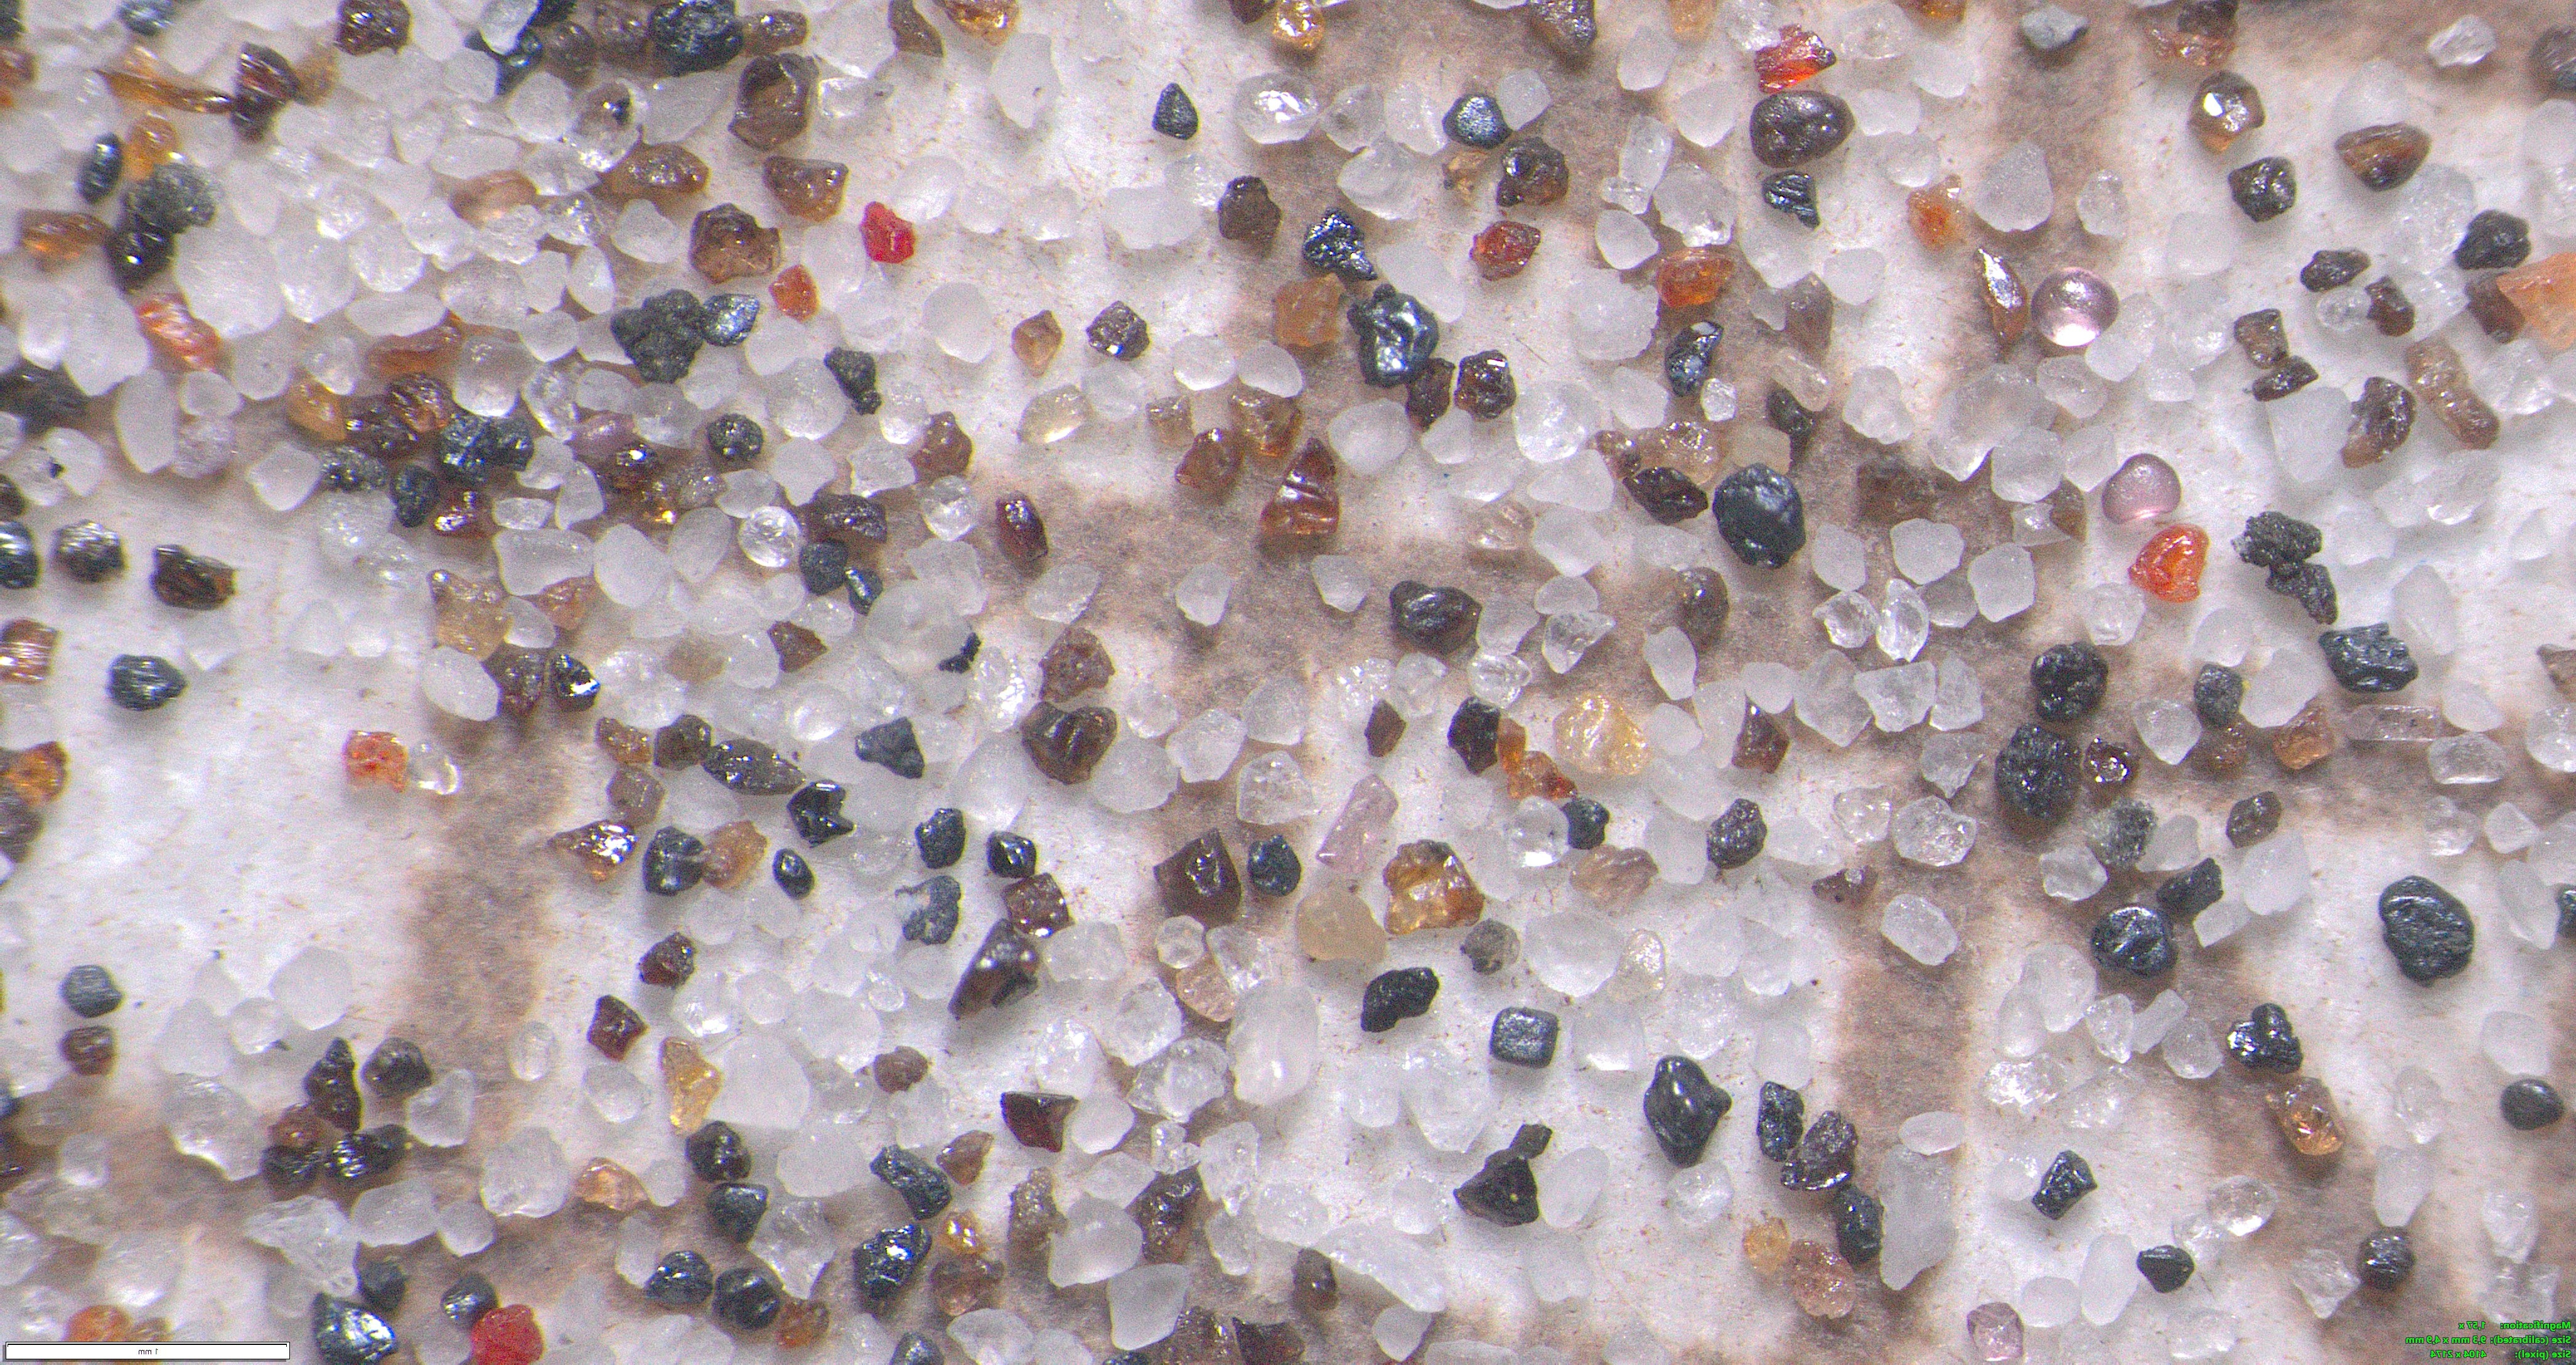
\includegraphics[width=\textwidth]{figure/hasilFlipHorizontal.jpg}
        \caption{Hasil \textit{Flip} Horizontal ($\curvearrowright$)}
        \label{fig:3.hasilFlipHorizontal}
    \end{subfigure}
    \hfill
    \begin{subfigure}[b]{0.475\textwidth}
        \centering
        \includegraphics[width=\textwidth]{figure/hasilFlipVertical.jpg}
        % \caption{Hasil \textit{Flip} Vertical ($\shortdownarrow$)}
        \caption{Hasil \textit{Flip} Vertical (\protect$\downarrow$)}
        % \caption{Hasil \textit{Flip} Vertical ($\downarrow$)}

        \label{fig:3.hasilFlipVertical}
    \end{subfigure}
    \caption{Hasil \textit{Flip} Data}
    \label{fig:3.HasilFlipData}
\end{figure}

\subsubsection*{\textnormal{2. \textit{Rotate}}}
Pada tahapan ini, data citra mikroskop diolah dengan menerapkan teknik augmentasi \textit{random rotation} yang memutar citra pada rentang sudut tertentu, seperti $-15^{\circ}$ hingga $+15^{\circ}$ untuk menambah variasi data pelatihan \cite{RotateBatik}. Teknik ini digunakan agar model dapat mengenali objek mineral kasiterit dari berbagai sudut pandang tanpa kehilangan informasi penting pada citra. Tujuan dari \textit{rotate} ini adalah untuk memperkaya sudut pandang data dan membantu model dalam mengenali objek mineral kasiterit yang mungkin muncul dalam orientasi berbeda di bawah mikroskop. Contoh hasil penerapan teknik \textit{rotate} dengan sudut rotasi sebesar $15^{\circ}$ dapat dilihat pada Gambar \ref{fig:3.HasilRotateData} berikut. \par

\begin{figure}[H]
    \centering
    % Baris pertama: dua gambar sejajar
    \begin{subfigure}[b]{0.475\textwidth}
        \centering
        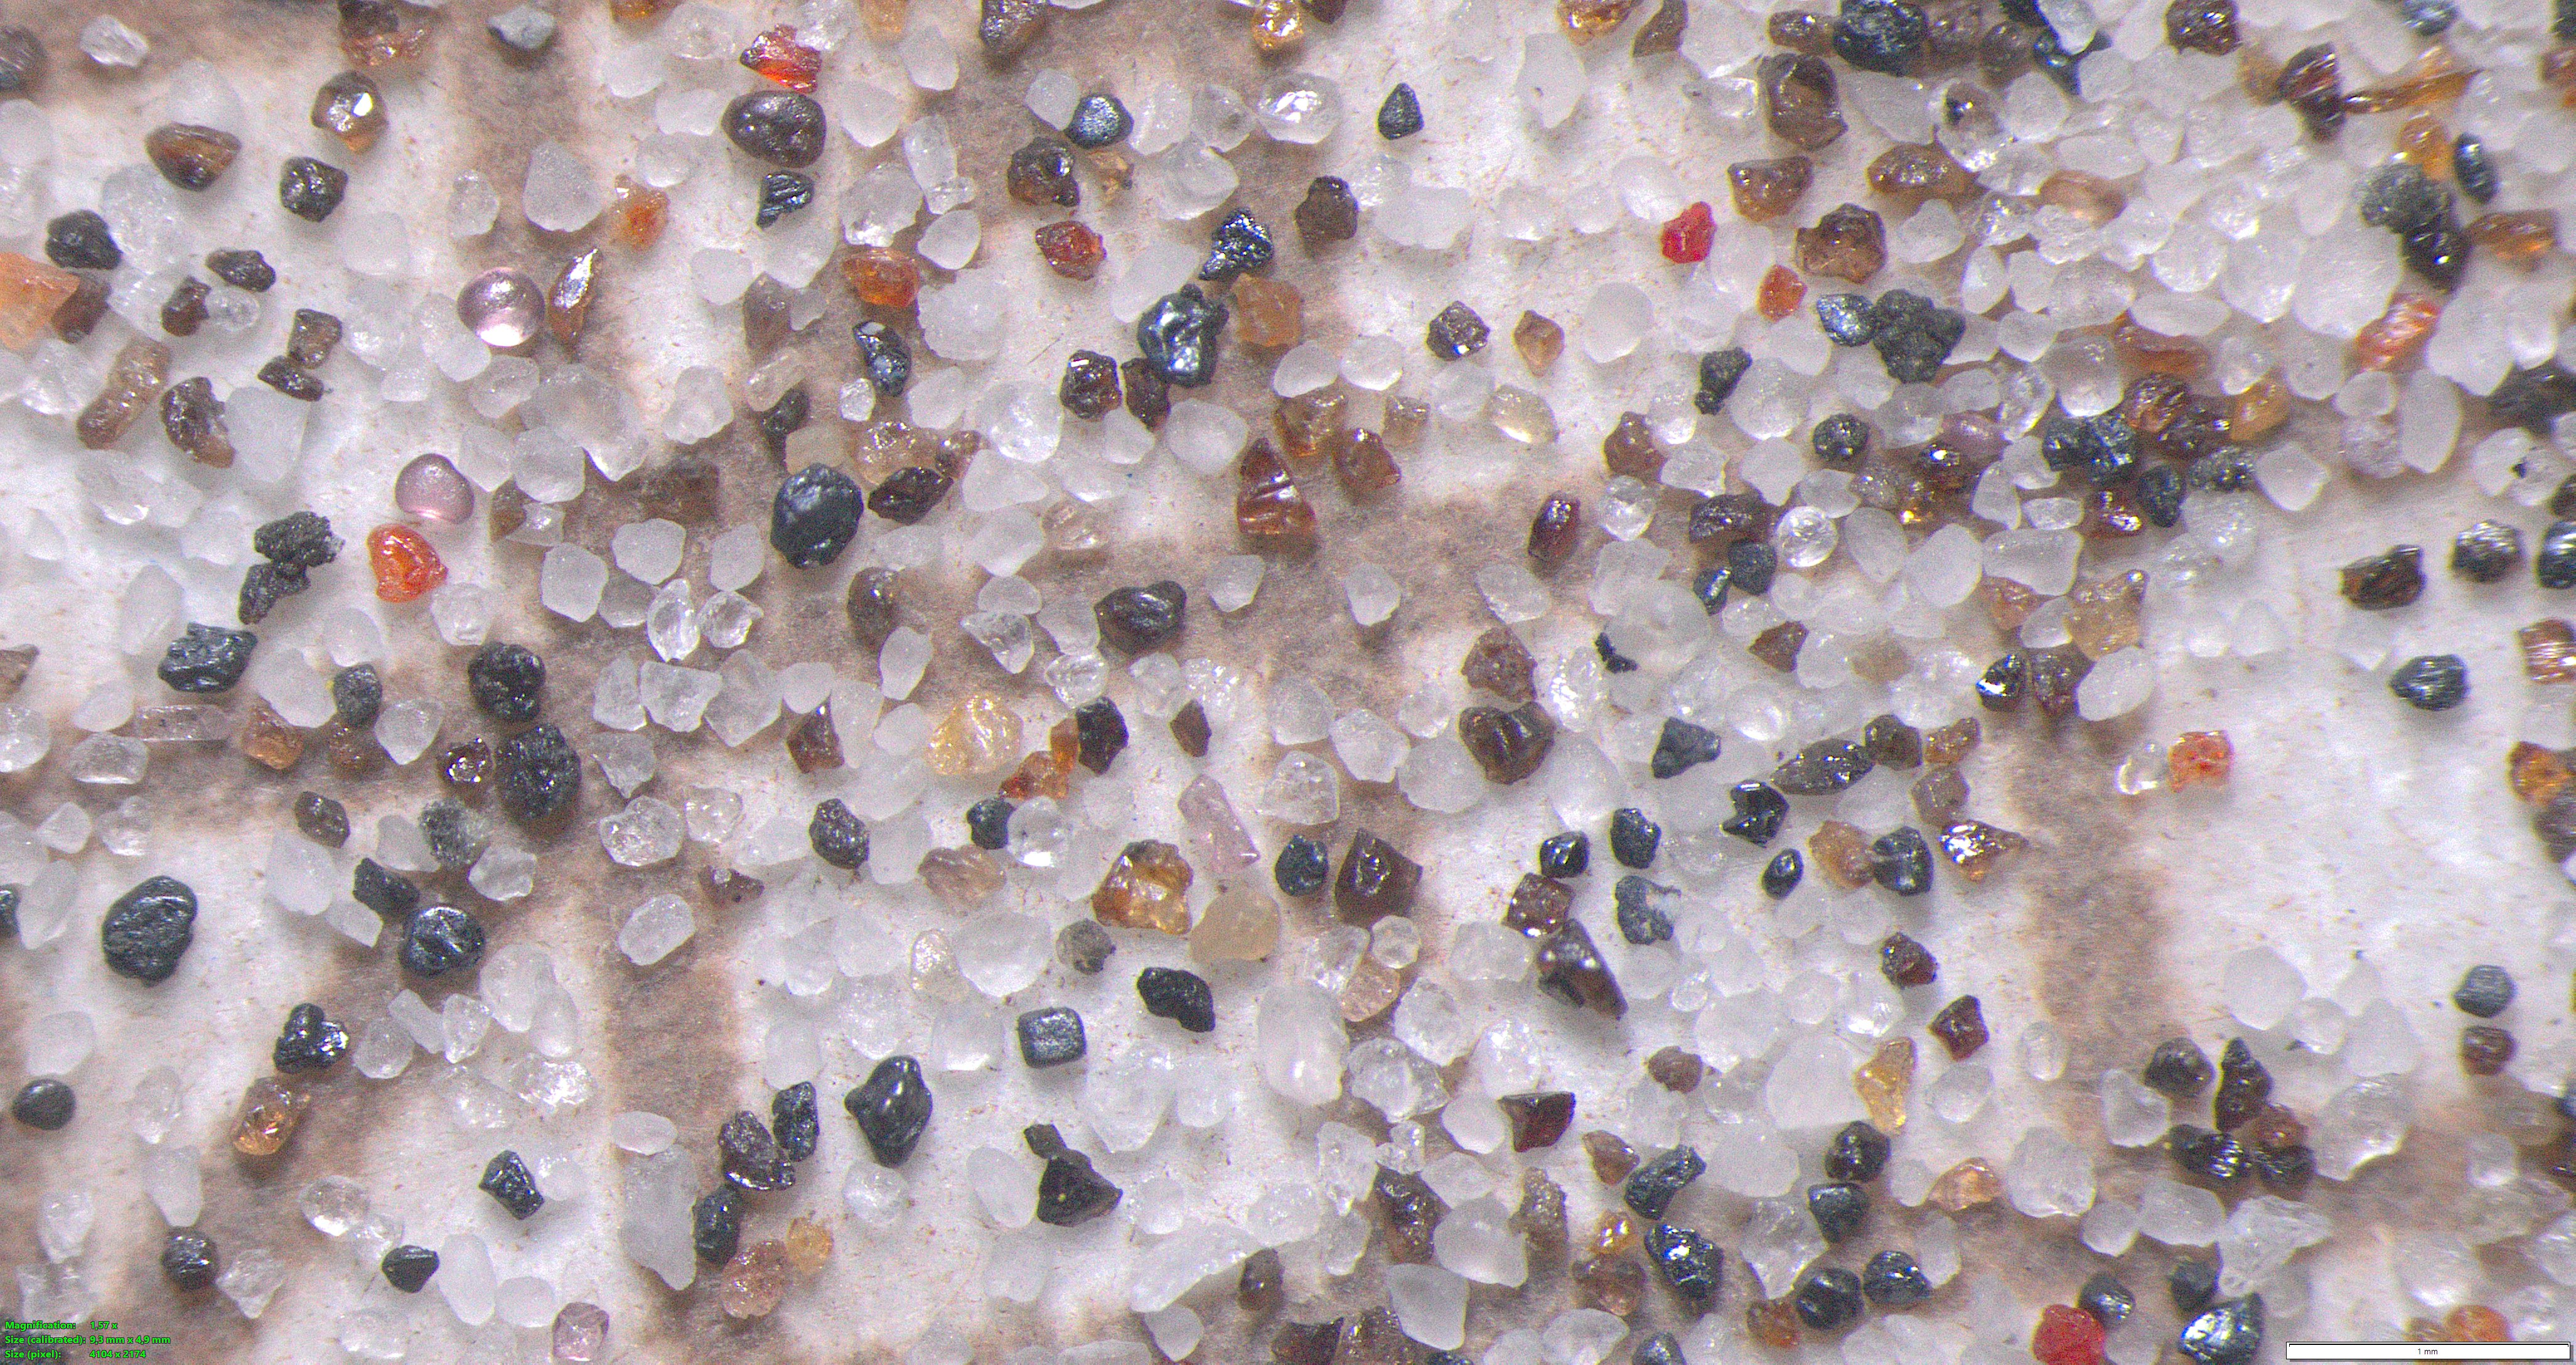
\includegraphics[width=\textwidth]{figure/sebeleumResize.jpg}
        \caption{Citra Awal tanpa \textit{Rotate}}
        \label{fig:3.RotateAwal}
    \end{subfigure}
    \hfill
    \begin{subfigure}[b]{0.475\textwidth}
        \centering
        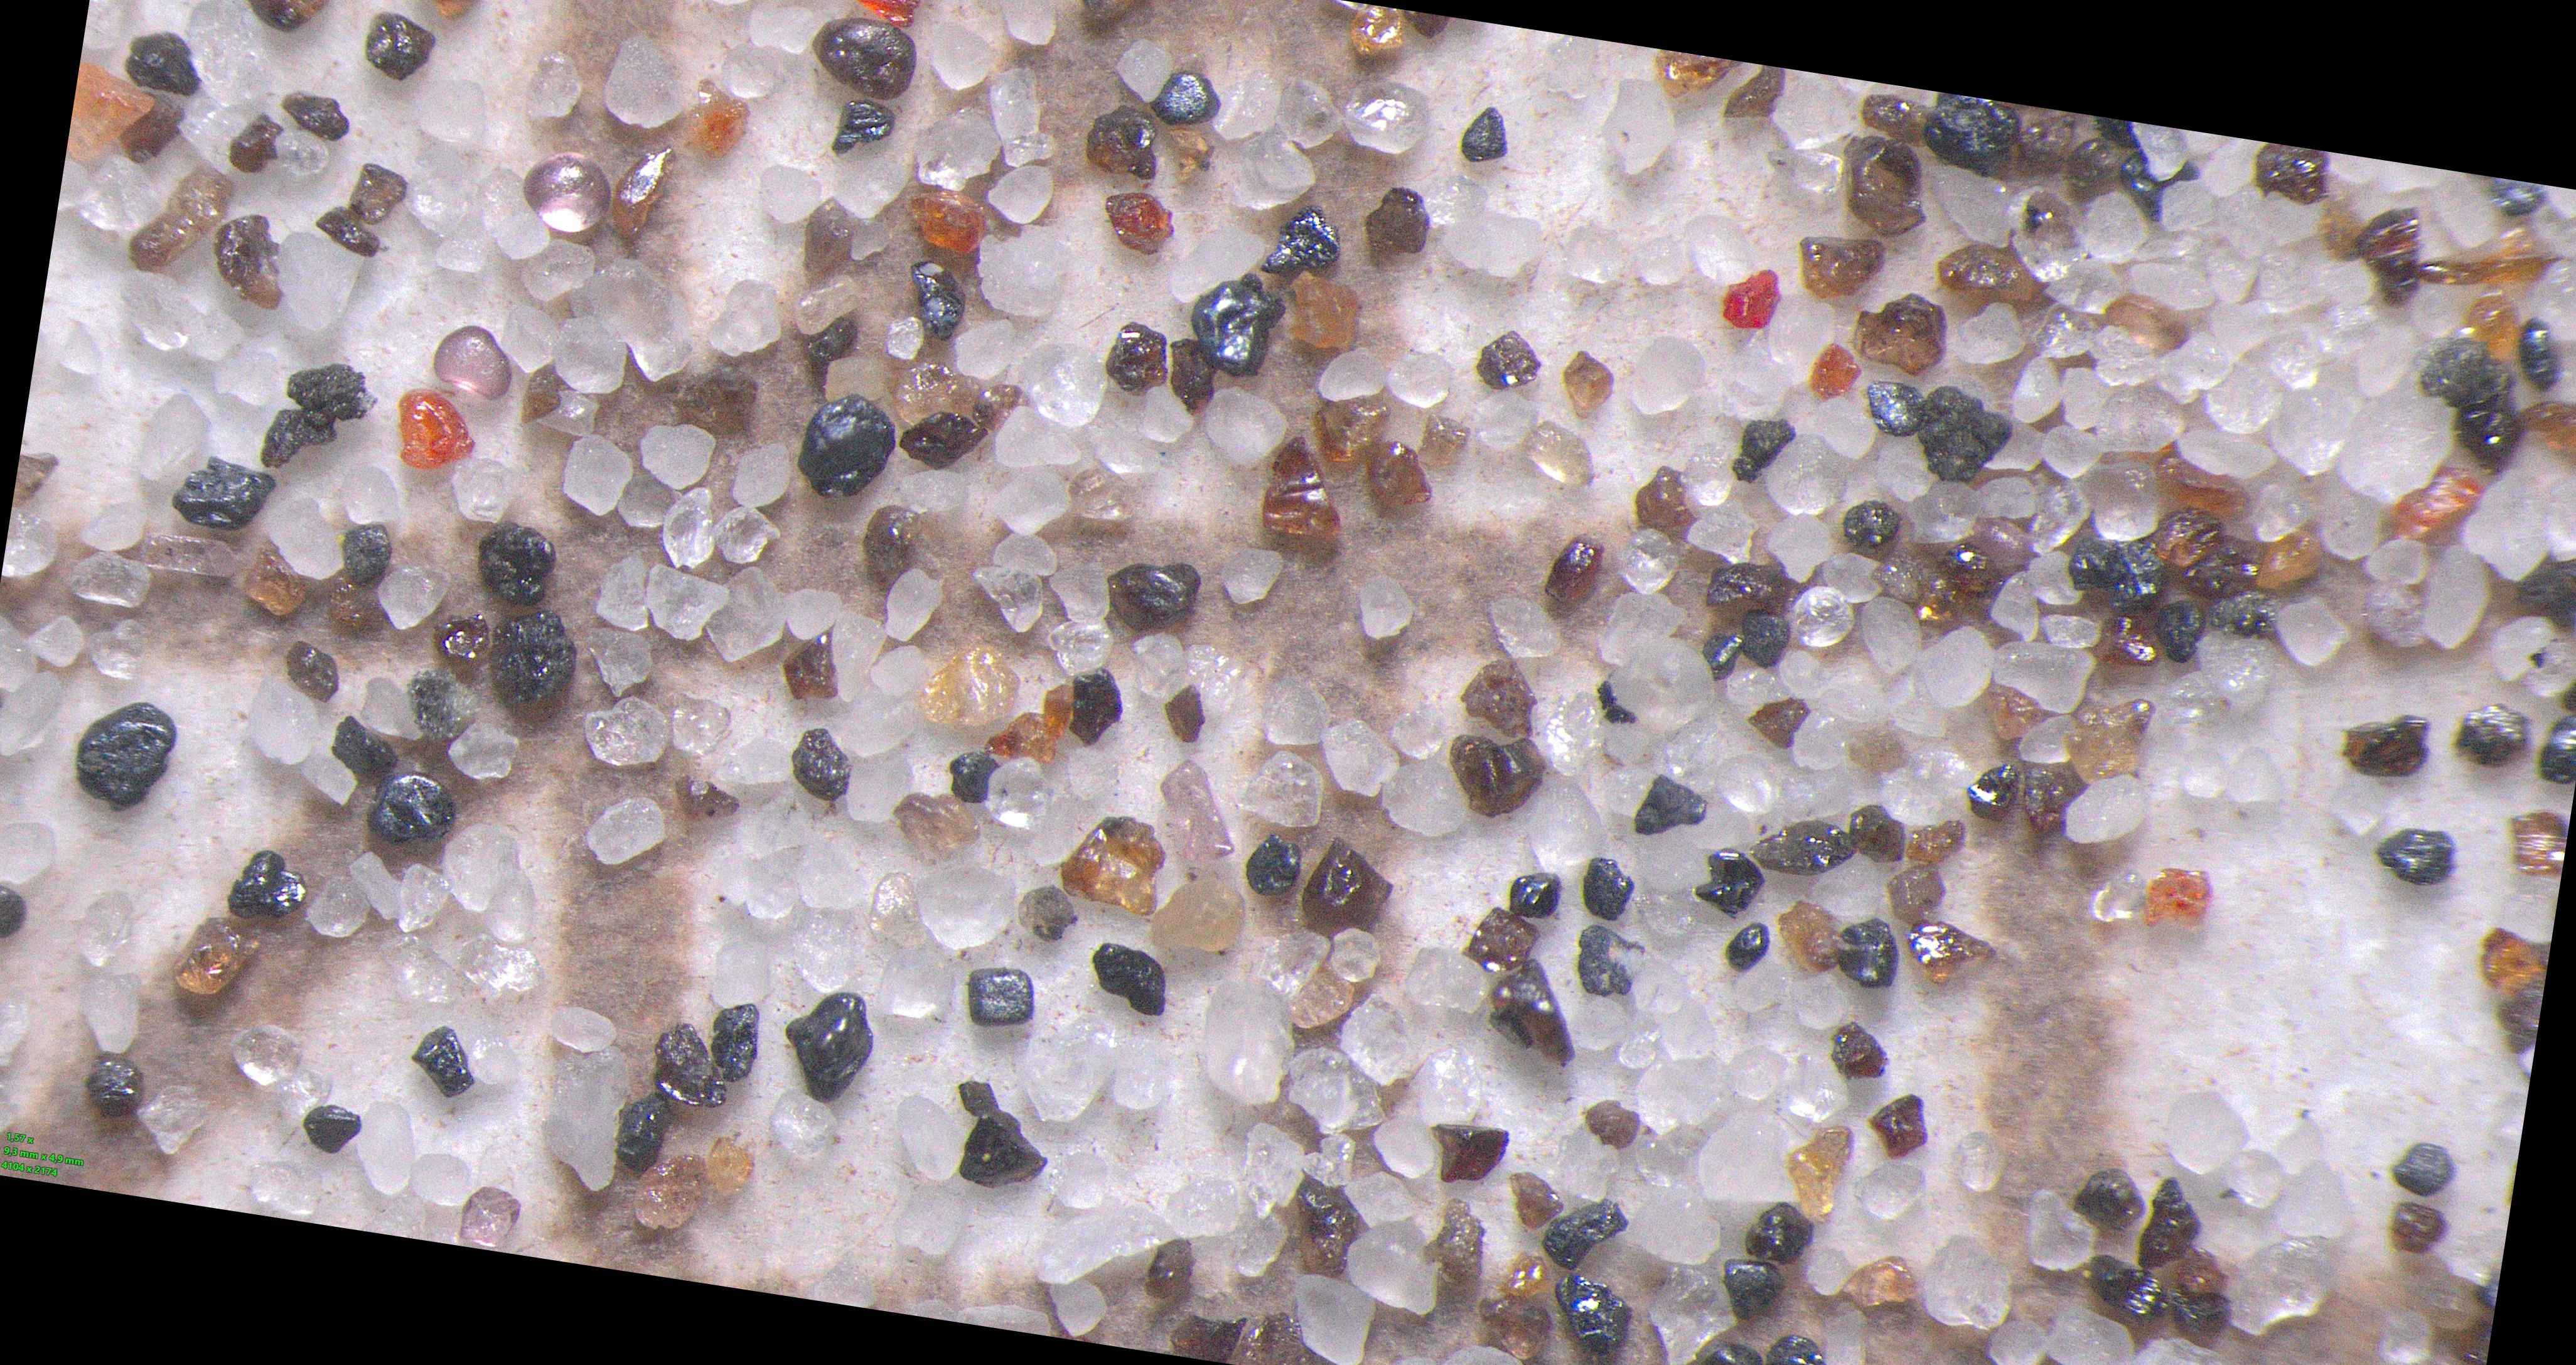
\includegraphics[width=\textwidth]{figure/hasilRotate.jpg}
        \caption{Hasil \textit{Rotate} dengan 15\textdegree}
        \label{fig:3.HasilRotate}
    \end{subfigure}

	\caption{Hasil \textit{Rotate} Data}
    \label{fig:3.HasilRotateData}
\end{figure}

\subsubsection*{\textnormal{3. \textit{Gaussian Noise}}}
Pada tahapan ini, data citra mikroskop diolah dengan menerapkan teknik augmentasi \textit{Gaussian noise} yang menambahkan derau acak pada citra untuk meningkatkan ketahanan model terhadap gangguan visual. Penambahan \textit{noise} dilakukan dengan intensitas rendah agar tidak mengubah karakteristik warna asli mineral, tetapi tetap memberikan variasi kecil yang dapat memperkuat kemampuan generalisasi model terhadap perubahan pencahayaan dan fluktuasi sensor. \textit{Gaussian noise} diterapkan menggunakan nilai variansi sebesar 0{,}2 \cite{GaussianNoise0.2}, sehingga derau yang ditambahkan bersifat halus dan tidak mengganggu struktur visual mineral kasiterit. Contoh hasil penerapan teknik \textit{Gaussian noise} dengan variansi 0{,}2 ditunjukkan pada Gambar \ref{fig:3.HasilGaussianNoiseData} berikut. \par

\begin{figure}[H]
    \centering
    % Baris pertama: dua gambar sejajar
    \begin{subfigure}[b]{0.475\textwidth}
        \centering
        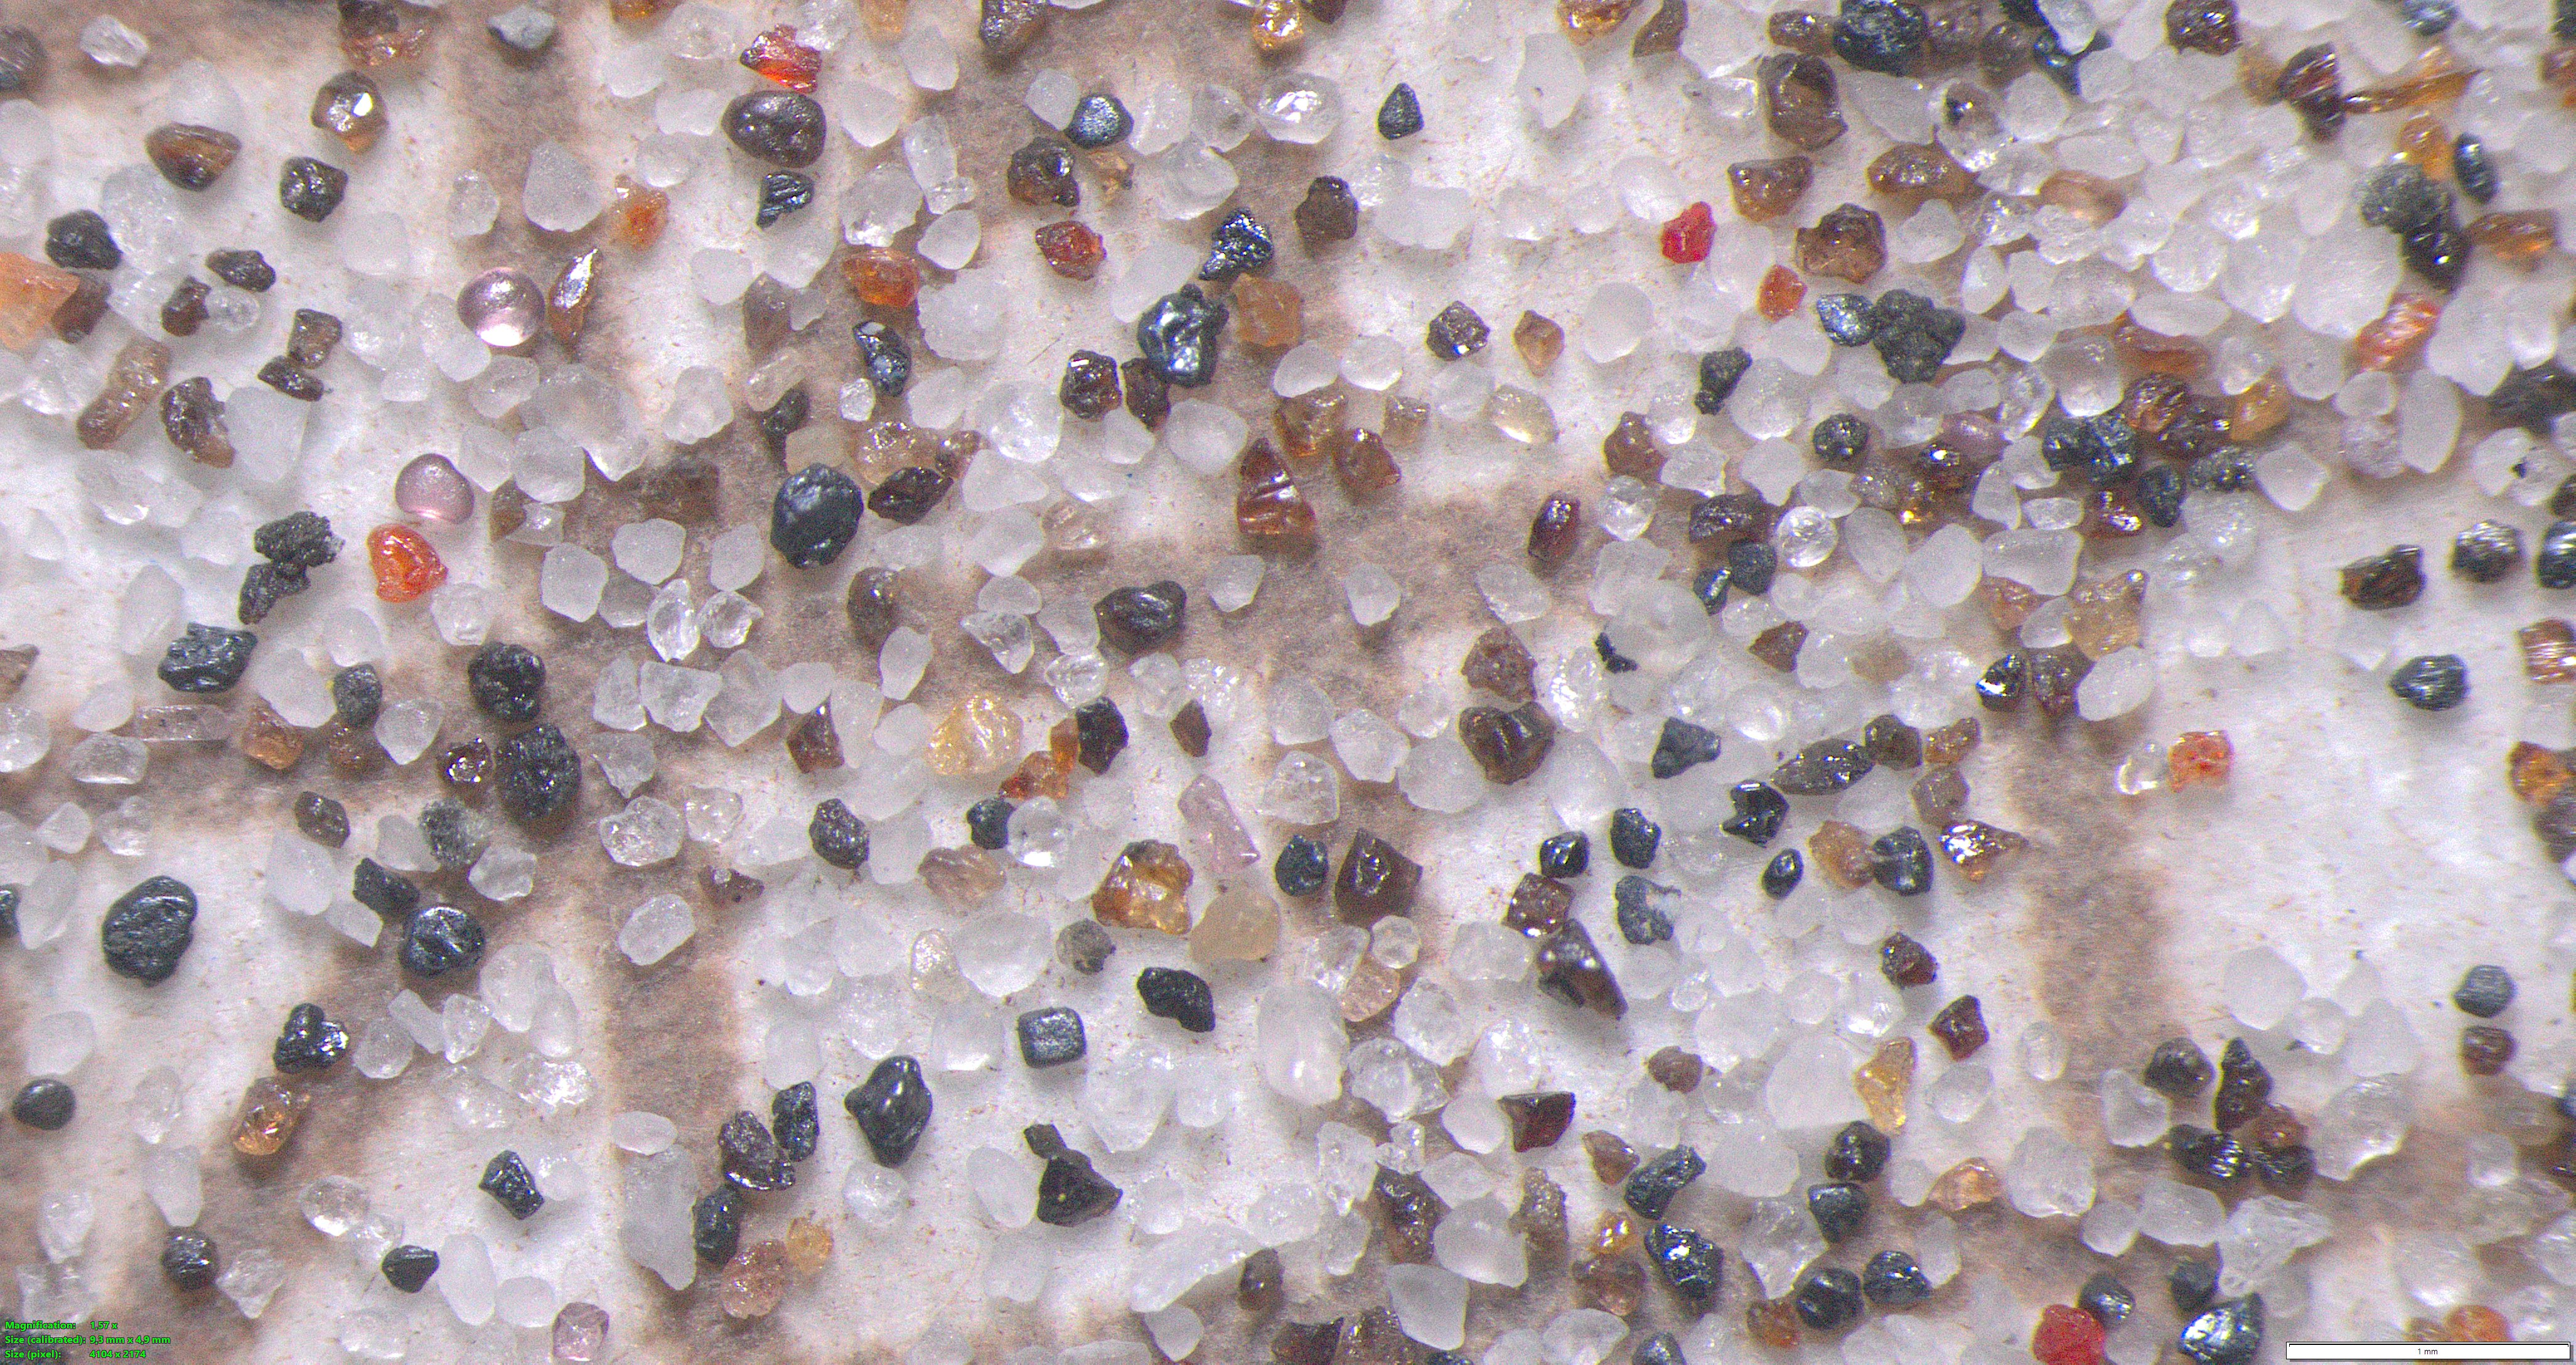
\includegraphics[width=\textwidth]{figure/sebeleumResize.jpg}
        \caption{Citra Awal tanpa \textit{Gaussian Noise}}
        \label{fig:3.GaussianAwal}
    \end{subfigure}
    \hfill
    \begin{subfigure}[b]{0.475\textwidth}
        \centering
        \includegraphics[width=\textwidth]{figure/hasilGaussianNoise.jpg}
        \caption{Hasil \textit{Gaussian Noise} dengan variansi 0{,}2}
        \label{fig:3.HasilGaussianNoise}
    \end{subfigure}

	\caption{Hasil \textit{Gaussian Noise} Data}
    \label{fig:3.HasilGaussianNoiseData}
\end{figure}

\subsubsection{\textit{Normalization}}
Pada tahapan ini, data citra mikroskop diolah dengan menerapkan teknik \textit{normalization} yang menyesuaikan rentang nilai piksel citra agar berada dalam skala tertentu, biasanya antara 0 hingga 1. Teknik ini digunakan untuk memastikan bahwa semua fitur pada citra memiliki kontribusi yang seimbang selama proses pelatihan model. Dengan melakukan \textit{normalization}, model dapat belajar lebih efektif karena perbedaan skala nilai piksel tidak akan memengaruhi proses pembelajaran.  \par

\begin{table}[h!]
\centering
\caption{Contoh piksel sebelum dinormalisasi}
\renewcommand{\arraystretch}{1.2} % Mengatur jarak antar baris
\setlength{\tabcolsep}{10pt} % Mengatur jarak antar kolom
\label{table:3.contoh-normalization}
\begin{tabular}{|c|c|c|c|c|}
\hline
\textbf{(i,j)} & \textbf{$(0,j)$} & \textbf{$(1,j)$} & \textbf{$(2,j)$} & \textbf{$(3,j)$} \\ \hline
$(i,0)$ & 123 & 45 & 200 & 89 \\ \hline
$(i,1)$ & 15  & 255 & 87 & 142 \\ \hline
$(i,2)$ & 64  & 31 & 219 & 176 \\ \hline
$(i,3)$ & 92  & 8 & 73 & 240 \\ \hline
\end{tabular}
\end{table}

Sebagai contoh, nilai piksel sebesar $X = 123$ yang terletak pada posisi baris ke-1 dan kolom ke-1 (indeks [0,0]) pada Tabel \ref{table:3.contoh-normalization} digunakan untuk perhitungan normalisasi. Berdasarkan Persamaan \ref{eq:2.normalization}, dengan $X_{min} = 0$ dan $X_{max} = 255$. Maka nilai piksel setelah dilakukan normalisasi ($X_{normal}$) dapat dihitung sebagai berikut: 

\begin{align*}
    X_{normal} &= \frac{X - X_{min}}{X_{max} - X_{min}} \\[0.5em]
    X_{normal} &= \frac{123 - 0}{255 - 0} \\[0.5em]
    X_{normal} &= \frac{123}{255} \\[0.5em]
    X_{normal} &= 0{,}482 \\[0.5em]
\end{align*}

Dengan demikian, nilai piksel pada indeks [0,0] sebesar $123$ setelah dilakukan normalisasi menjadi $0{,}482$, yang menunjukkan bahwa intensitas piksel tersebut telah diskalakan ke dalam rentang 0--1 sehingga siap digunakan dalam proses pelatihan model.

\begin{table}[h!]
\centering
\caption{Hasil piksel sebelum di normalisasii}
\renewcommand{\arraystretch}{1.2} % Mengatur jarak antar baris
\setlength{\tabcolsep}{10pt} % Mengatur jarak antar kolom
\label{table:3.Hasil-normalization}
\begin{tabular}{|c|c|c|c|c|}
\hline
\textbf{(i,j)} & \textbf{$(0,j)$} & \textbf{$(1,j)$} & \textbf{$(2,j)$} & \textbf{$(3,j)$} \\ \hline
$(i,0)$ & 0{,}482 & 0{,}176 & 0{,}784 & 0{,}349 \\ \hline
$(i,1)$ & 0{,}059 & 1{,}000 & 0{,}341 & 0{,}557 \\ \hline
$(i,2)$ & 0{,}251 & 0{,}122 & 0{,}859 & 0{,}690 \\ \hline
$(i,3)$ & 0{,}361 & 0{,}031 & 0{,}286 & 0{,}941 \\ \hline
\end{tabular}
\end{table}


\subsection{Pengembangan Model} \label{III.LangkahPengembanganModel}
Pada penelitian ini, alur pengembangan model yang digunakan dalam identifikasi mineral kasiterit pada citra mikroskop menggunakan \textit{Mask} R-CNN ditunjukkan pada Gambar \ref{fig:3.AlurPengembanganModel} berikut.\par

\begin{figure}[H] % Kalau menggunakan H, posisi gambar akan tepat dibawah teks
    \centering
    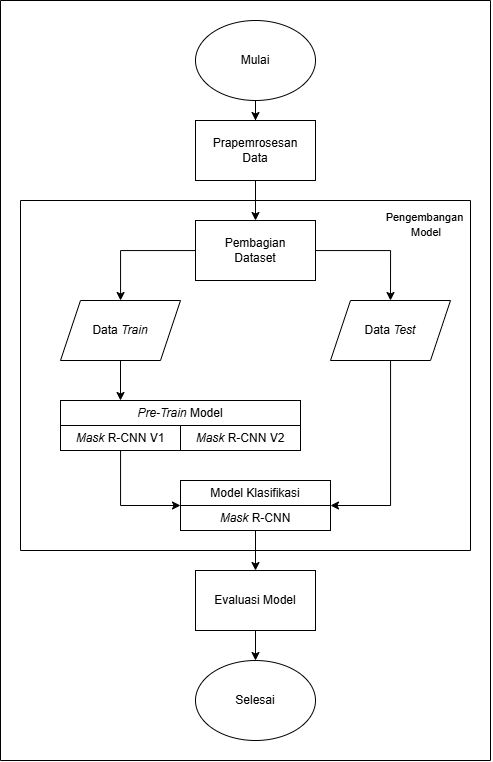
\includegraphics[width=0.73\textwidth]{figure/pengembanganModelfinal.png}
    \caption{Alur Pengembangan Model}
    \label{fig:3.AlurPengembanganModel}
\end{figure}

\subsubsection{Pembagian Data}
Pada tahapan ini, dataset yang telah melalui proses prapemrosesan dibagi menjadi data latih (\textit{training}) dan data validasi (\textit{validation}) menggunakan metode \textit{k-fold cross validation} dengan nilai $K=5$. Metode ini membagi dataset menjadi lima bagian (\textit{fold}) yang seimbang, di mana setiap \textit{fold} secara bergantian berperan sebagai data uji, sementara empat \textit{fold} lainnya digunakan untuk pelatihan. Dengan rasio pembagian 80:20 pada setiap iterasi, yaitu 80\% data digunakan untuk pelatihan dan 20\% data digunakan untuk pengujian, sehingga seluruh data memperoleh kesempatan untuk menjadi data uji setidaknya satu kali. \par

\subsubsection{Pelatihan Model}
Pada tahap ini, arsitektur \textit{Mask} R-CNN dilatih menggunakan data latih yang telah disiapkan sebelumnya. Penelitian terdahulu dengan topik serupa telah berhasil mengidentifikasi konfigurasi arsitektur yang efektif untuk tugas segmentasi objek mineral \cite{mineralogiMaskRCNNSolo} \cite{OreSegmentation2} \cite{unet}. Penelitian ini menggunakan dua \textit{Model Pre-trained} dari arsitektur \textit{Mask} R-CNN, yaitu dengan \textit{backbone} ResNet50 FPN versi V1 dan versi V2. Versi V2 tidak mengubah struktur arsitektur inti dari V1, tetapi meningkatkan performa melalui proses pelatihan ulang yang lebih mutakhir, meliputi penerapan augmentasi skala besar (\textit{Large Scale Jittering}), penggunaan normalisasi yang lebih stabil, penerapan regularisasi \textit{DropPath}, serta pemanfaatan \textit{optimizer AdamW} \cite{maskrcnnv2}. Strategi pelatihan yang lebih modern tersebut menghasilkan bobot \textit{pre-trained} yang lebih representatif dan akurat, dengan nilai \textit{mask} $mAP$ sebesar 41{,}8 pada V2, lebih tinggi dibandingkan V1 yang memperoleh 34{,}6 \cite{pytorchWebsite}.

Kedua arsitektur tersebut diuji pada dua bentuk model, yaitu model \textit{standar} dan model \textit{amodal}. Model \textit{standar} menggunakan \textit{mask head} konvensional yang hanya memprediksi bagian objek yang terlihat (\textit{visible mask}), sedangkan model \textit{amodal} dilengkapi dengan cabang jaringan tambahan (\textit{amodal mask head}) yang dirancang khusus untuk merekonstruksi bentuk utuh objek meskipun sebagian tertutup oleh objek lain (oklusi). 

\begin{figure}[H]
    \centering
    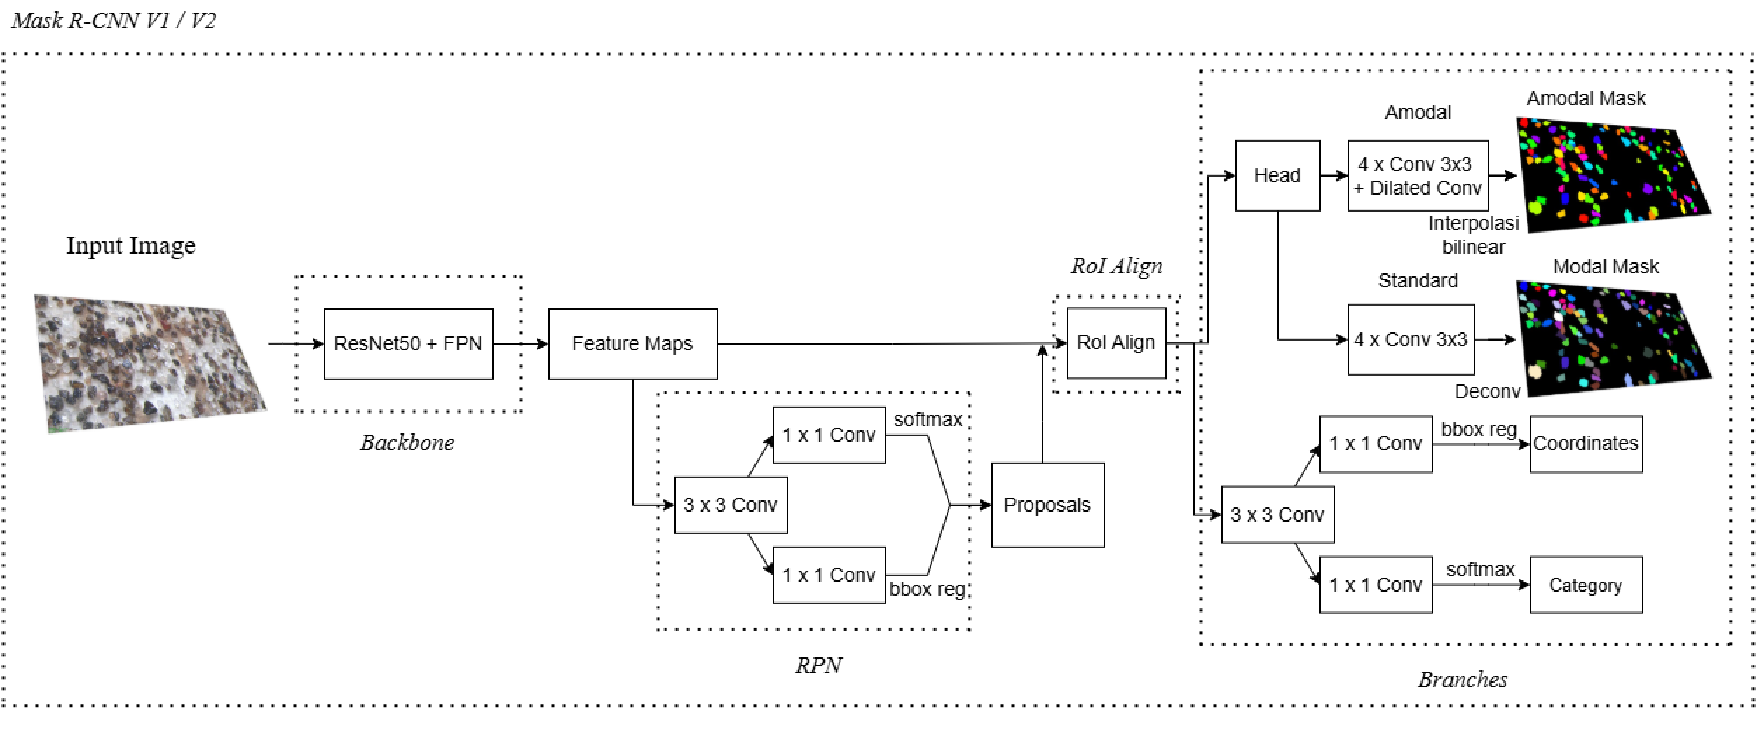
\includegraphics[page=1, width=1\textwidth]{doc/arsitektur ammodal.drawio2.pdf}
    \caption{Arsitektur \textit{Mask} R-CNN dengan cabang \textit{Amodal Instance Segmentation}}
    \label{fig:amodal-architecture}
\end{figure}

Sebagaimana ditunjukkan pada Gambar \ref{fig:amodal-architecture}, cabang \textit{amodal mask head} memiliki struktur arsitektur yang berbeda dibandingkan dengan \textit{modal mask head} standar. Pada cabang modal, arsitektur yang digunakan mengikuti struktur konvensional yang terdiri dari tumpukan lapisan konvolusi dan dilanjutkan dengan lapisan dekonvolusi untuk proses \textit{upsampling} \cite{MaskRcnnIEEE11}. Sementara itu, cabang amodal mengintegrasikan empat lapisan konvolusi $3 \times 3$ dengan lapisan \textit{dilated convolution}. Penerapan \textit{dilated convolution} bertujuan untuk memperluas \textit{receptive field} secara eksponensial tanpa mengorbankan resolusi spasial, sehingga mampu menangkap informasi konteks global pada berbagai skala \cite{dilatedConv}. Hal ini krusial bagi model dalam memprediksi kelanjutan struktur butiran mineral kasiterit yang teroklusi. Selanjutnya, lapisan \textit{upsample} berbasis interpolasi bilinear diterapkan untuk meningkatkan resolusi \textit{mask} secara halus guna menjaga konsistensi bentuk dan kontinuitas spasial objek, diikuti oleh lapisan konvolusi $1 \times 1$ untuk menghasilkan probabilitas piksel pada setiap lokasi \textit{mask amodal}. Melalui kombinasi komponen tersebut, model mampu merekonstruksi bentuk utuh mineral kasiterit meskipun sebagian areanya tertutup oleh butiran lain, yang pada akhirnya meningkatkan akurasi identifikasi pada kondisi oklusi dalam citra mikroskop. \par

Selain variasi model, kedua arsitektur juga dikombinasikan dengan dua algoritma optimasi berbeda, yaitu \textit{Stochastic Gradient Descent} (SGD) dan \textit{Adam}. Kombinasi antara variasi model dan algoritma optimasi tersebut menghasilkan delapan konfigurasi pelatihan sebagaimana ditunjukkan pada Tabel~\ref{table:3.konfigurasi-model}.
 
\begin{longtable}{|>{\centering\arraybackslash}p{0.25\textwidth}|>{\centering\arraybackslash}p{0.25\textwidth}|>{\centering\arraybackslash}p{0.25\textwidth}|} % Longtable berguna agar tabel dapat terpotong di halaman baru
    \caption{Variasi konfigurasi pelatihan}
        \label{table:3.konfigurasi-model}\\
        \hline
        \textbf{\textit{Model Pre-trained}} & \textbf{\textit{Model}} & \textbf{\textit{Optimizer}} \\
        \hline
        \endfirsthead % Header tabel untuk halaman pertama
        \hline
        \textbf{\textit{Model Pre-trained}} & \textbf{\textit{Model}} & \textbf{\textit{Optimizer}} \\
        \hline
        \endhead % Header tabel untuk halaman selanjutnya (repeat header row)
        \multirow{4}{*}{\shortstack{\textit{Mask} R-CNN \\ResNet50 FPN V1}} & \multirow{2}{*}{\textit{Amodal}} & SGD \\
        \cline{3-3}
         & & \textit{Adam} \\
        \cline{2-3}
         & \multirow{2}{*}{\textit{Standar}} & SGD \\
        \cline{3-3}
         & & \textit{Adam} \\
        \hline
        \multirow{4}{*}{\shortstack{\textit{Mask} R-CNN \\ResNet50 FPN V2}} & \multirow{2}{*}{\textit{Amodal}} & SGD \\
        \cline{3-3}
         & & \textit{Adam} \\
        \cline{2-3}
         & \multirow{2}{*}{\textit{Standar}} & SGD \\
        \cline{3-3}
         & & \textit{Adam} \\
        \hline
\end{longtable}

\subsection{Evaluasi Model} \label{III.LangkahEvaluasiModel}
Pada tahap evaluasi, setiap variasi konfigurasi pelatihan pada model \textit{Mask} R-CNN diuji untuk menilai pengaruhnya terhadap kinerja model. Evaluasi dilakukan menggunakan data validasi yang telah dipisahkan sebelumnya agar hasil yang diperoleh bersifat objektif dan bebas dari bias data latih. Kinerja model diukur berdasarkan dua metrik utama, yaitu \textit{Average Precision} (AP) dan \textit{Intersection over Union} (IoU), yang digunakan untuk menilai tingkat akurasi deteksi serta kualitas segmentasi objek. Metrik AP dihitung pada tiga \textit{threshold} yang berbeda, yaitu \APfifty, \APseventyfive, dan \APrangefifty, untuk mengukur performa model pada tingkat keketatan deteksi yang bervariasi. Begitu pula dengan IoU, yang dihitung pada \IoUfifty, \IoUseventyfive, dan \IoUrangefifty guna mengevaluasi kualitas tumpang tindih antara prediksi dan \textit{ground truth} pada berbagai tingkat presisi. Evaluasi ini juga mempertimbangkan penerapan teknik \textit{amodal instance segmentation} untuk menguji kemampuan model mengenali objek yang saling menutupi pada citra uji. Hasil evaluasi dari setiap konfigurasi kemudian dibandingkan untuk menentukan kombinasi konfigurasi pelatihan yang memberikan performa terbaik. \par


\subsection{Hasil dan Pembahasan} \label{III.LangkahHasilDanPembahasan}
Pada tahap ini, setelah model \textit{Mask} R-CNN selesai dilakukan evaluasi, diperoleh hasil perbandingan dari setiap variasi konfigurasi pelatihan yang telah diuji. Hasil performa dari setiap variasi konfigurasi pelatihan akan dibandingkan untuk mengetahui model mana yang paling optimal dalam melakukan identifikasi mineral kasiterit pada citra mikroskop berdasarkan metrik \textit{Average Precision} (AP) dan \textit{Intersection over Union} (IoU) termasuk pada penerapan teknik \textit{amodal instance segmentation} untuk mendeteksi butiran yang saling menutupi. Berdasarkan hasil analisis, akan diperoleh kesimpulan mengenai efektivitas masing-masing variasi konfigurasi pelatihan dalam melakukan identifikasi mineral kasiterit. Selain itu, kesimpulan juga dapat menjadi dasar untuk penelitian atau pengembangan selanjutnya. \par

\section{Alat dan Bahan Tugas Akhir} \label{III.Alat dan Bahan}
Alat dan Bahan yang digunakan dalam penelitian tugas akhir ini adalah sebagai berikut: \par

\subsection{Alat} \label{III.Alat}
Alat yang digunakan untuk melakukan penelitian tugas akhir ini adalah sebagai berikut: \par
\begin{enumerate}[noitemsep]
	\item Laptop ASUS TUF FX517ZC dengan sistem operasi Windows 11 Home 64-bit, RAM 16 GB DDR5, prosesor Intel® Core™ i7-12650H, kartu grafis NVIDIA® GeForce RTX™ 3050 4GB GDDR6.
	\item Visual Studio Code versi 1.109.0 dan Antigravity versi 1.107.0 untuk melakukan pengembangan kode program dan penulisan dokumentasi.
	\item Github untuk menyimpan kode program, dataset dan dokumentasi secara daring.
	\item Notion untuk mencatat revisi dan informasi, sekaligus untuk manajemen proyek.
	\item Labelme with SAM \cite{Wada_Labelme_Image_Polygonal} untuk melakukan segmentasi data citra mikroskop.
	\item Runpod untuk melakukan pelatihan model \textit{Mask} R-CNN menggunakan GPU RTX PRO 6000.
\end{enumerate}

\subsection{Bahan} \label{III.Bahan}
Bahan yang digunakan pada penelitian ini adalah dataset citra mikroskop mineral kasiterit yang bersumber dari Laboratorium Eksplorasi PT. Timah Tbk yang berlokasi di Kota Pangkalpinang, Bangka Belitung \cite{PTTimahWebsite}.\par

\section{Metode Pengembangan} \label{III.Metode}
Pada penelitian ini, metode pengembangan yang digunakan adalah \textit{Mask} R-CNN untuk mengidentifikasi dan dapat melakukan segmentasi mineral kasiterit pada citra mikroskop dengan membandingkan beberapa variasi konfigurasi pelatihan serta menerapkan teknik \textit{amodal instance segmentation} agar model dapat mengenali bentuk utuh butiran mineral yang saling menutupi pada citra mikroskop. 

\section{Ilustrasi Perhitungan Metode} \label{III.Ilustrasi}
Berikut adalah ilustrasi perhitungan yang dilakukan pada penelitian ini. \par

\subsection{\textit{Loss Function Mask} R-CNN}
Bagian ini menjelaskan secara rinci proses perhitungan fungsi kerugian (\textit{loss function}) pada arsitektur \textit{Mask R-CNN}, yang terdiri dari tiga komponen utama: \textit{Classification Loss} ($L_{\text{cls}}$), \textit{Bounding Box Regression Loss} ($L_{\text{box}}$), dan \textit{Mask Loss} ($L_{\text{mask}}$). Ketiga komponen ini bekerja bersama untuk mengoptimalkan performa deteksi dan segmentasi objek pada citra. 
Fungsi kerugian total ($L$) pada \textit{Mask R-CNN} dapat dihitung dengan menjumlahkan ketiga komponen tersebut, seperti yang ditunjukkan pada \ref{eq:2.maskrcnn}. \par

% \begin{align*}
%     L &= L_{\text{cls}} + L_{\text{box}} + L_{\text{mask}} \\[0.5em]
% \end{align*}

Sebagai ilustrasi penerapan perhitungan fungsi kerugian secara keseluruhan, digunakan contoh data yang terdiri dari hasil perhitungan ketiga komponen loss, yaitu $L_{\text{cls}} = 0{,}27002$, $L_{\text{box}} = 0{,}0023$, dan $L_{\text{mask}} = 0{,}1923$. Dengan memasukkan nilai-nilai tersebut ke dalam rumus total loss pada \textit{Mask} R-CNN, diperoleh perhitungan akhir sebagai berikut: \par

\begin{align*}
    L &= L_{\text{cls}} + L_{\text{box}} + L_{\text{mask}} \\[0.5em]
    L &= 0{,}27002 + 0{,}0023 + 0{,}1923 \\[0.5em]
    L &= 0{,}46462
\end{align*}

\subsubsection{Perhitungan $L_{\text{cls}}$ \textit{(Classification Loss)}}

Fungsi kerugian klasifikasi digunakan untuk mengukur seberapa baik model dalam memprediksi label kelas untuk setiap \textit{Region of Interest} (RoI). Pada Mask R-CNN, fungsi ini biasanya menggunakan \textit{binary cross-entropy loss} yang membandingkan nilai prediksi ($p_i$) dengan label sebenarnya ($p_i^*$) menggunakan logaritma natural yang di definisikan sebagai $\log$, seperti yang ditunjukkan pada \ref{eq:2.cls_loss}.  \par

% \begin{align*}
%     L_{\text{cls}} &= \frac{1}{N_{\text{cls}}} \sum_i \big(-p_i^* \log p_i - (1 - p_i^*) \log (1 - p_i)\big) \\[0.5em]
% \end{align*}

Tabel berikut menunjukkan data contoh lima RoI yang digunakan dalam ilustrasi perhitungan ini, masing-masing memiliki nilai prediksi ($p_i$), label kebenaran ($p_i^*$), dan ukuran mask yang seragam ($4\times4$), seperti yang ditunjukkan pada Tabel \ref{table:3.contoh-data-roi-loss} berikut. \par

\begin{table}[H]
\centering
\caption{Contoh Data RoI untuk Ilustrasi Perhitungan \textit{Classification Loss} R-CNN}
\renewcommand{\arraystretch}{1.3}
\label{table:3.contoh-data-roi-loss}
\begin{tabular}{|c|c|c|>{\centering\arraybackslash}m{2.2cm}|}
\hline
\textbf{RoI} & \textbf{$p_i$ (prediksi)} & \textbf{$p_i^*$ (label)} & \textbf{Ukuran Mask} \\ 
\hline
1 & 0,80 & 1 & $4 \times 4$ \\ 
\hline
2 & 0,60 & 1 & $4 \times 4$ \\ 
\hline
3 & 0,20 & 0 & $4 \times 4$ \\ 
\hline
4 & 0,75 & 1 & $4 \times 4$ \\ 
\hline
5 & 0,10 & 0 & $4 \times 4$ \\ 
\hline
\end{tabular}
\end{table}

Jumlah total RoI yang digunakan adalah lima, sehingga $N_{\text{cls}} = 5$. Perhitungan dilakukan dengan memasukkan nilai-nilai prediksi dan label ke dalam rumus \textit{cross-entropy loss} untuk tiap RoI. Dalam perhitungan ini, kita akan menggunakan data $p_i = 0{,}8$ dan $p_i^* = 1$ sebagai contoh untuk RoI pertama. \par 

\begin{align*}
    L_{\text{cls}} &= \frac{1}{N_{\text{cls}}} \sum_i \big(-p_i^* \log p_i - (1 - p_i^*) \log (1 - p_i)\big) \\[0.5em]
     &= \frac{1}{5} \sum_{i=1}^{5} \big(-1 \cdot \log 0{,}8 - (1 - 1) \log (1 - 0{,}8)\big) \\[0.5em]
     &= \frac{1}{5} \sum_{i=1}^{5} \big(-1 \cdot \log 0{,}8 - 0 \cdot \log (1 - 0{,}8)\big) \\[0.5em]
     &= \frac{1}{5} \sum_{i=1}^{5} \big(-\log 0{,}8 \big) \\[0.5em]
     &= \frac{1}{5} \sum_{i=1}^{5} 0{,}2231 \\[0.5em]
     &= 0{,}2231 \\[0.5em]
\end{align*}

Berikut hasil lengkap perhitungan per-RoI untuk $L_{\text{cls}}$.

\begin{table}[H]
\centering
\caption{Perhitungan $L_{\text{cls}}$ (klasifikasi)}
\renewcommand{\arraystretch}{1.3}
\label{table:3.loss-cls}
\begin{tabular}{|c|c|c|>{\centering\arraybackslash}m{3.7cm}|c|}
\hline
\textbf{RoI} & \textbf{$p_i$ (prediksi)} & \textbf{$p_i^*$ (label)} & \textbf{Rumus terapan} & \textbf{Hasil} \\ 
\hline
1 & 0,80 & 1 & $-\log 0{,}8$ & 0{,}2231 \\ 
\hline
2 & 0,60 & 1 & $-\log 0{,}6$ & 0{,}5108 \\ 
\hline
3 & 0,20 & 0 & $-\log (1-0{,}2) = -\log 0{,}8$ & 0{,}2231 \\ 
\hline
4 & 0,75 & 1 & $-\log 0{,}75$ & 0{,}2877 \\ 
\hline
5 & 0,10 & 0 & $-\log (1-0{,}1) = -\log 0{,}9$ & 0{,}1054 \\ 
\hline
\end{tabular}
\end{table}

Dengan menjumlahkan seluruh hasil dan membaginya dengan jumlah RoI, diperoleh nilai rata-rata $L_{\text{cls}}$ sebesar:

\begin{align*}
    L_{\text{cls}} &= \frac{0{,}2231 + 0{,}5108 + 0{,}2231 + 0{,}2877 + 0{,}1054}{5} \\[0.5em]
     &= \frac{1{,}3501}{5} \\[0.5em]
     &= 0{,}27002
\end{align*}

\subsubsection{Perhitungan $L_{\text{box}}$ \textit{(Bounding Box Regression Loss)}}
Bagian ini menghitung kesalahan antara koordinat prediksi kotak pembatas ($t_i$) dan nilai kebenarannya ($t_i^*$). Komponen ini menggunakan fungsi $L_1^{\text{smooth}}$, yang merupakan versi halus dari \textit{L1 loss} untuk menghindari perubahan gradien mendadak, seperti yang ditunjukkan pada \ref{eq:2.box_loss}.

% \begin{align*}
%     L_{\text{box}} &= \frac{\lambda}{N_{\text{box}}} \sum_i p_i^* \cdot L_1^{\text{smooth}}(t_i - t_i^*) \\[0.5em]
% \end{align*}

Data berikut menunjukkan tiga RoI dengan label positif ($p_i^* = 1$), yang digunakan untuk menghitung $L_{\text{box}}$ sebanyak 3 RoI, seperti yang ditunjukkan pada Tabel \ref{table:3.contoh-data-box-loss-pos} berikut.

\begin{table}[H]
\centering
\caption{Contoh Data RoI (hanya label = 1) dengan $t_i$, $t_i^*$ dan hasil bbox ($t_i - t_i^*$)}
\renewcommand{\arraystretch}{1.3}
\label{table:3.contoh-data-box-loss-pos}
\begin{tabular}{|c|c|>{\centering\arraybackslash}m{2.4cm}|>{\centering\arraybackslash}m{2.6cm}|}
\hline
\textbf{RoI} & \textbf{$p_i^*$} & \textbf{$t_i$ (prediksi)} & \textbf{$t_i^*$ (ground-truth)} \\ 
\hline
1 & 1 & [0{,}55; \,0{,}45; \newline\,0{,}62; \,0{,}52] & [0{,}45; \,0{,}50; \newline\,0{,}60; \,0{,}55] \\ 
\hline
2 & 1 & [0{,}68; \,-0{,}22; \newline\,0{,}55; \,0{,}21] & [0{,}60; \,-0{,}20; \newline\,0{,}50; \,0{,}20] \\ 
\hline
4 & 1 & [0{,}55; \,0{,}44; \newline\,-0{,}28; \,-0{,}16] & [0{,}50; \,0{,}40; \newline\,-0{,}25; \,-0{,}15] \\ 
\hline
\end{tabular}
\end{table}

Perhitungan selisih $t_i - t_i^*$ menghasilkan vektor $d$, yang selanjutnya digunakan dalam fungsi $L_1^{\text{smooth}}$. Karena semua komponen memiliki nilai $|d| < 1$, maka digunakan rumus $\frac{1}{2}d^2$ untuk setiap elemen. Sebagai contoh perhitungan untuk RoI pertama menggunakan  ${t_i} = [0{,}55; \,0{,}45; \,0{,}62; \,0{,}52]$ dan ${t_i^*} = [0{,}45; \,0{,}50; \,0{,}60; \,0{,}55]${,}

\begin{align*}
    {t_i - t_i^*} &= [0{,}55; \,0{,}45; \,0{,}62; \,0{,}52] - [0{,}45; \,0{,}50; \,0{,}60; \,0{,}55] \\[0.5em]
    {t_i - t_i^*} &= [0{,}10; \,-0{,}05; \,0{,}02; \,-0{,}03] \\[0.5em]
\end{align*}

Dari hasil selisih ($t_i - t_i^*$) atau $d$ pada perhitungan di atas, dapat dilihat bahwa semua nilai $d$ memenuhi kondisi $|d| < 1$. Oleh karena itu, fungsi $L_1^{\text{smooth}}(t_i - t_i^*)$ yang digunakan adalah $\frac{1}{2}d^2$ untuk setiap komponen vektor $d$. Sebagai contoh, perhitungan dilakukan untuk komponen pertama vektor $d$ yaitu $d[0] = 0{,}10$ sebagai berikut:

% \begin{align*}
%     {t_i - t_i^*} &= d = [0.10; \,-0.05; \,0.02; \,-0.03] \\[0.5em]
% \end{align*}

\begin{align*}
    d[0] &= 0{,}10 = |0{,}10| = \frac{1}{2}(0{,}10)^2 = 0{,}0050 \\
    % d[1] &= -0.05 = |0.05| = \frac{1}{2}(0.05)^2 = 0.00125 \\[0.5em]
    % d[2] &= 0.02 = |0.02| = \frac{1}{2}(0.02)^2 = 0.0002 \\[0.5em]
    % d[3] &= -0.03 = |0.03| = \frac{1}{2}(0.03)^2 = 0.00045 \\[0.5em]
\end{align*}

Setelah menghitung nilai smooth $L_1$ untuk setiap komponen vektor $d$, diperoleh empat nilai yaitu $0{,}0050$; $0{,}00125$; $0{,}0002$; dan $0{,}00045$. Selanjutnya, hasil dari semua komponen tersebut dijumlahkan untuk memperoleh total nilai $L_1^{\text{smooth}}(t_i - t_i^*)$ untuk RoI pertama. Perhitungan dilakukan sebagai berikut:

\begin{align*}
    L_1^{\text{smooth}}(t_i - t_i^*) &= 0{,}0050 + 0{,}00125 + 0{,}0002 + 0{,}00045 \\[0.5em]
     &= 0{,}0069 \\[0.5em]
     &= 0{,}0050 + 0{,}00125 + 0{,}0002 + 0{,}00045 \\[0.5em]
     &= 0{,}0069 \\[0.5em]
\end{align*}

Dengan cara yang sama, perhitungan $L_1^{\text{smooth}}(t_i - t_i^*)$ dilakukan untuk RoI kedua dan keempat, menghasilkan nilai 0{,}0035 dan 0{,}0018 secara berurutan. Selanjutnya, nilai-nilai ini digunakan untuk menghitung total $L_{\text{box}}$ dengan memasukkan nilai-nilai tersebut ke dalam rumus utama. \\
\begin{align*}
    L_{\text{box}} &= \frac{\lambda}{N_{\text{box}}} \sum_i p_i^* \cdot L_1^{\text{smooth}}(t_i - t_i^*) \\[0.5em]
     &= \frac{1}{3} \sum_{i=1}^{3} 1 \cdot 0{,}0069 \\[0.5em]
     &= \frac{1}{3} \cdot 0{,}0069 \\[0.5em]
     &= 0{,}0023 \\[0.5em]
\end{align*}

Tabel \ref{table:3.hasil-data-box-loss-pos} berikut menunjukkan hasil perhitungan $L_{\text{box}}$ untuk setiap RoI dengan label positif ($p_i^* = 1$). Pada tabel tersebut dapat dilihat selisih antara prediksi dan ground truth ($t_i - t_i^*$), nilai $L_1^{\text{smooth}}$ untuk masing-masing RoI, serta kontribusi setiap RoI terhadap total $L_{\text{box}}$.

\begin{table}[H]
\centering
\caption{Hasil Akhir Perhitungan $L_{\text{box}}$}
\renewcommand{\arraystretch}{1.3}
\label{table:3.hasil-data-box-loss-pos}
\begin{tabular}{|c|>{\centering\arraybackslash}m{1.9cm}|>{\centering\arraybackslash}m{1.9cm}|>{\centering\arraybackslash}m{1.9cm}|>{\centering\arraybackslash}m{1.4cm}|c|}
\hline
\textbf{RoI} & \textbf{$t_i$} & \textbf{$t_i^*$} & \textbf{$t_i - t_i^*$ ($d$)} & \textbf{$L_1^{\text{smooth}}$} & \textbf{$L_{\text{box}}$} \\ 
\hline
1 & [0{,}55; \,0{,}45; \newline\,0{,}62; \,0{,}52] & [0{,}45; \,0{,}50; \newline\,0{,}60; \,0{,}55] & [0{,}10; \,-0{,}05; \newline\,0{,}02; \,-0{,}03] & 0{,}0069 & 0{,}0023 \\ 
\hline
2 & [0{,}68; \,-0{,}22; \newline\,0{,}55; \,0{,}21] & [0{,}60; \,-0{,}20; \newline\,0{,}50; \,0{,}20] & [0{,}08; \,-0{,}02; \newline\,0{,}05; \,0{,}01] & 0{,}0035 & 0{,}0012 \\ 
\hline
4 & [0{,}55; \,0{,}44; \newline\,-0{,}28; \,-0{,}16] & [0{,}50; \,0{,}40; \newline\,-0{,}25; \,-0{,}15] & [0{,}05; \,0{,}04; \newline\,-0{,}03; \,-0{,}01] & 0{,}0018 & 0{,}0006 \\ 
\hline
\end{tabular}
\end{table}

\subsubsection{Perhitungan $L_{\text{mask}}$ \textit{(Mask Loss)}}
Komponen ini berfungsi mengukur seberapa akurat model dalam menghasilkan segmentasi piksel objek dibandingkan dengan mask sebenarnya. Setiap piksel dihitung menggunakan \textit{binary cross-entropy} berdasarkan probabilitas prediksi $\hat{y}_{ij}$ dan label kebenaran $y_{ij}$, seperti yang ditunjukkan pada \ref{eq:2.maskloss}.

% \begin{align*}
% 	L_{\text{mask}} &= -\frac{1}{m^2}\sum_{1 \leq i,j \leq m}
% 	\Big[ y_{ij} \log \hat{y}^{k}_{ij} + (1 - y_{ij}) \log (1 - \hat{y}^{k}_{ij}) \Big] \\[0.5em]
% \end{align*}

Ukuran mask yang digunakan adalah $4 \times 4$, sehingga jumlah piksel total $m^2 = 16$. Berikut contoh representasi nilai label dan prediksi yang digunakan: \\

\begin{align*}
y_{ij} &=
\begin{bmatrix}
1 & 1 & 0 & 0 \\
1 & 1 & 0 & 0 \\
1 & 0 & 0 & 0 \\
0 & 0 & 0 & 0
\end{bmatrix}, \quad
\hat{y}_{ij} =
\begin{bmatrix}
0{,}9 & 0{,}8 & 0{,}2 & 0{,}1 \\
0{,}9 & 0{,}7 & 0{,}3 & 0{,}2 \\
0{,}8 & 0{,}4 & 0{,}1 & 0{,}1 \\
0{,}2 & 0{,}1 & 0{,}1 & 0{,}0
\end{bmatrix}
\\[0.5em]
\end{align*}

Untuk menghitung \textit{mask loss} secara detail, perhitungan dilakukan untuk setiap piksel pada mask yang berukuran $4 \times 4$. Setiap piksel diidentifikasi menggunakan index $(i,j)$ yang dimulai dari $(0,0)$ hingga $(3,3)$, di mana $i$ mewakili index baris dan $j$ mewakili index kolom. Perhitungan \textit{loss} untuk setiap piksel dilakukan dengan terlebih dahulu memecah rumus utama menjadi bentuk yang lebih sederhana, yaitu $\text{loss}_{ij}$. Dengan demikian, rumus \textit{mask loss} dapat ditulis ulang menjadi:

\begin{align*}
    L_{\text{mask}} &= \frac{1}{m^2}\sum_{1 \leq i,j \leq m} \text{loss}_{ij} \\[0.5em]
\end{align*}

Di mana nilai $\text{loss}_{ij}$ untuk setiap piksel pada mask dihitung secara terpisah menggunakan rumus di bawah ini yang menerapkan fungsi \textit{binary cross-entropy} untuk membandingkan nilai prediksi dengan nilai sebenarnya:

\begin{align*}
    % \\[0.5em]
	{\text{loss}_{ij}} &= -\Big[ y_{ij} \log \hat{y}^{k}_{ij} + (1 - y_{ij}) \log (1 - \hat{y}^{k}_{ij}) \Big] \\[0.5em]
\end{align*}

Sebagai contoh, perhitungan untuk piksel pertama dengan index $(0,0)$ dilakukan menggunakan nilai $y_{ij} = 1$ dan $\hat{y}_{ij} = 0{,}9$ sebagai berikut:

\begin{align*}
    % \\[0.5em]
	{\text{loss}_{ij}} &= -\Big[ y_{ij} \log \hat{y}^{k}_{ij} + (1 - y_{ij}) \log (1 - \hat{y}^{k}_{ij}) \Big] \\[0.5em]
	 &= -\Big[ 1 \cdot \log 0{,}9 + (1 - 1) \log (1 - 0{,}9) \Big] \\[0.5em]
	 &= -\Big[ 1 \cdot \log 0{,}9 + 0 \cdot \log (0{,}1) \Big] \\[0.5em]
	 &= -\Big[\log 0{,}9 \Big] \\[0.5em]
	 &= 0{,}1057\\[0.5em]
\end{align*}

Dengan cara yang sama, perhitungan dilakukan untuk setiap piksel pada seluruh index ($i = 0, 1, 2, 3$) menggunakan rumus yang telah ditetapkan. Adapun hasil perhitungan untuk salah satu indeks yaitu indeks 0, adalah sebagai berikut. \par

\textbf{Index 0 ($i = 0$)}
\begin{table}[H]
\centering
% \caption{data tabel Index 0 ($i = 0$)}
\renewcommand{\arraystretch}{1.3}
\label{table:3.data-index-0}
\begin{tabular}{|c|c|c|c|c|}
\hline
\textbf{(i,j)} & \textbf{$y_{ij}$} & \textbf{$\hat{y}_{ij}$} & \textbf{Bentuk Rumus} & \textbf{Hasil} \\
\hline
(0,0) & 1 & 0{,}9 & $-\log(0{,}9)$ & 0{,}1054 \\ \hline
(0,1) & 1 & 0{,}8 & $-\log(0{,}8)$ & 0{,}2231 \\ \hline
(0,2) & 0 & 0{,}2 & $-\log(1-0{,}2)=-\log(0{,}8)$ & 0{,}2231 \\ \hline
(0,3) & 0 & 0{,}1 & $-\log(1-0{,}1)=-\log(0{,}9)$ & 0{,}1054 \\
\hline
\end{tabular}
\end{table}

% \textbf{Index 1 ($i = 1$)}
% \begin{table}[H]
% \centering
% % \caption{data tabel Index 1 ($i = 1$)}
% \renewcommand{\arraystretch}{1.3}
% \label{table:3.data-index-1}
% \begin{tabular}{|c|c|c|c|c|}
% \hline
% \textbf{(i,j)} & \textbf{$y_{ij}$} & \textbf{$\hat{y}_{ij}$} & \textbf{Bentuk Rumus} & \textbf{Hasil} \\
% \hline
% (1,0) & 1 & 0.9 & $-\log(0.9)$ & 0.1054 \\ \hline
% (1,1) & 1 & 0.7 & $-\log(0.7)$ & 0.3567 \\ \hline
% (1,2) & 0 & 0.3 & $-\log(1-0.3)=-\log(0.7)$ & 0.3567 \\ \hline
% (1,3) & 0 & 0.2 & $-\log(1-0.2)=-\log(0.8)$ & 0.2231 \\
% \hline
% \end{tabular}
% \end{table}

% \textbf{Index 2 ($i = 2$)}
% \begin{table}[H]
% \centering
% % \caption{data tabel Index 2 ($i = 2$)}
% \renewcommand{\arraystretch}{1.3}
% \label{table:3.data-index-2}
% \begin{tabular}{|c|c|c|c|c|}
% \hline
% \textbf{(i,j)} & \textbf{$y_{ij}$} & \textbf{$\hat{y}_{ij}$} & \textbf{Bentuk Rumus} & \textbf{Hasil} \\
% \hline
% (2,0) & 1 & 0.8 & $-\log(0.8)$ & 0.2231 \\ \hline
% (2,1) & 0 & 0.4 & $-\log(1-0.4)=-\log(0.6)$ & 0.5108 \\ \hline
% (2,2) & 0 & 0.1 & $-\log(1-0.1)=-\log(0.9)$ & 0.1054 \\ \hline
% (2,3) & 0 & 0.1 & $-\log(1-0.1)=-\log(0.9)$ & 0.1054 \\
% \hline
% \end{tabular}
% \end{table}

% \textbf{Index 3 ($i = 3$)}
% \begin{table}[H]
% \centering
% % \caption{data tabel Index 3 ($i = 3$)}
% \renewcommand{\arraystretch}{1.3}
% \label{table:3.data-index-3}
% \begin{tabular}{|c|c|c|c|c|}
% \hline
% \textbf{(i,j)} & \textbf{$y_{ij}$} & \textbf{$\hat{y}_{ij}$} & \textbf{Bentuk Rumus} & \textbf{Hasil} \\
% \hline
% (3,0) & 0 & 0.2 & $-\log(1-0.2)=-\log(0.8)$ & 0.2231 \\ \hline
% (3,1) & 0 & 0.1 & $-\log(1-0.1)=-\log(0.9)$ & 0.1054 \\ \hline
% (3,2) & 0 & 0.1 & $-\log(1-0.1)=-\log(0.9)$ & 0.1054 \\ \hline
% (3,3) & 0 & 0.0 & $-\log(1-0.0)=-\log(1)=0$ & 0.0000 \\
% \hline
% \end{tabular}
% \end{table}

% di index (3,3), y = 0 dan ŷ = 0 → model yakin ini latar belakang, dan benar → loss = 0.

Setelah menghitung nilai $\text{loss}_{ij}$ untuk setiap piksel pada seluruh index, langkah selanjutnya adalah menjumlahkan hasil perhitungan per index. Penjumlahan ini dilakukan dengan menambahkan semua nilai $\text{loss}_{ij}$ pada setiap baris ($i = 0, 1, 2, 3$) untuk mendapatkan total \textit{loss} pada masing-masing index. Adapun hasil perhitungan untuk salah satu $\text{loss}_{ij}$, yaitu $\text{loss}_{0j}$ pada index 0, adalah sebagai berikut. \par

\begin{align*}
    \sum_{j=0}^{3}\text{loss}_{0j} &= 0{,}1054 + 0{,}2231 + 0{,}2231 + 0{,}1054 \\
     &= 0{,}6570 \\
\end{align*}

% \begin{align*}
%     \sum_{j=0}^{3}\text{loss}_{1j} &= 0.1054 + 0.3567 + 0.3567 + 0.2231 \\[0.5em]
%     \sum_{j=0}^{3}\text{loss}_{1j} &= 1.0419 \\[0.5em]
% \end{align*}

% \begin{align*}
%     \sum_{j=0}^{3}\text{loss}_{2j} &= 0.2231 + 0.5108 + 0.1054 + 0.1054 \\[0.5em]
%     \sum_{j=0}^{3}\text{loss}_{2j} &= 0.9447 \\[0.5em]
% \end{align*}

% \begin{align*}
%     \sum_{j=0}^{3}\text{loss}_{3j} &= 0.2231 + 0.1054 + 0.1054 + 0.0000 \\[0.5em]
%     \sum_{j=0}^{3}\text{loss}_{3j} &= 0.4339 \\[0.5em]
% \end{align*}

Setelah memperoleh nilai loss untuk masing-masing index dengan hasil 0{,}6570, 1{,}0419, 0{,}9447, dan 0{,}4339, langkah berikutnya adalah menjumlahkan seluruh nilai tersebut untuk mendapatkan total $\sum_{1 \leq i,j \leq m}{\text{loss}_{ij}}$. Penjumlahan ini dilakukan dengan menambahkan hasil loss dari index 0 hingga index 3 sebagai berikut. \par

\begin{align*}
    \sum_{1 \leq i,j \leq m}{\text{loss}_{ij}} &= 0,6570 + 1,0419 + 0,9447 + 0,4339 \\
     &= 3,0774 
\end{align*}

\subsubsection{Penghitungan Rata-rata per Piksel}

Setelah memperoleh total nilai loss dari seluruh piksel, langkah selanjutnya adalah menghitung rata-rata loss per piksel dengan membagi total loss terhadap jumlah piksel pada mask ($m^2$). Mengingat ukuran mask yang digunakan adalah $4 \times 4$, maka nilai $m = 4$ dan $m^2 = 16$. Perhitungan rata-rata loss per piksel dilakukan sesuai dengan rumus berikut:

\begin{align*}
    L_{\text{mask}} &= \frac{1}{m^2}\sum_{1 \leq i,j \leq m}{\text{loss}_{ij}} \\[0.5em]
     &= \frac{1}{4^2} \cdot 3{,}0774 \\[0.5em]
     &= \frac{1}{16} \cdot 3{,}0774 \\[0.5em]
     &= 0{,}1923 \\[0.5em]
\end{align*}

Dengan demikian, nilai $L_{\text{mask}}$ yang diperoleh adalah 0{,}1923, yang merepresentasikan rata-rata kesalahan prediksi mask untuk setiap piksel pada citra.

\subsection{Penentuan Level FPN}
Penentuan level pada \textit{Feature Pyramid Network} (FPN) dilakukan untuk menentukan pada level mana suatu \textit{Region of Interest} (RoI) akan diproses, yang bergantung pada ukuran objek ($w \times h$). Level FPN menentukan resolusi fitur yang digunakan, di mana objek kecil akan dianalisis pada level rendah (misalnya $P_2$), sedangkan objek besar menggunakan level tinggi (misalnya $P_5$), seperti yang ditunjukkan pada \ref{eq:2.maskloss}.  \\

% \begin{align*}
%     k = \left\lfloor k_0 + \log_2\!\left(\frac{\sqrt{wh}}{224}\right) \right\rfloor \\[0.5em]
% \end{align*}

Tabel \ref{table:3.data-fpn-level} menunjukkan contoh data tiga RoI dengan ukuran yang berbeda-beda, di mana nilai lebar ($w$) dan tinggi ($h$) untuk masing-masing RoI akan digunakan dalam perhitungan penentuan level FPN.

\begin{table}[H]
\centering
\caption{Data untuk Perhitungan Level FPN}
\renewcommand{\arraystretch}{1.3}
\label{table:3.data-fpn-level}
\begin{tabular}{|c|c|c|}
\hline
\textbf{RoI} & \textbf{$w$} & \textbf{$h$} \\ 
\hline
1 & 64 & 64 \\ 
\hline
2 & 128 & 128 \\ 
\hline
3 & 300 & 300 \\
\hline
\end{tabular}
\end{table}

dengan $k_0 = 4$ sebagai nilai default level dasar FPN, serta $w$ dan $h$ merupakan lebar dan tinggi RoI yang akan dihitung. Sebagai ilustrasi, perhitungan dilakukan untuk RoI pertama dengan menggunakan nilai $k_0 = 4$, $w = 64$, dan $h = 64$. Nilai-nilai ini kemudian disubstitusikan ke dalam rumus penentuan level FPN untuk memperoleh level yang sesuai.

\begin{align*}
    k &= \left\lfloor k_0 + \log_2\left(\frac{\sqrt{wh}}{224}\right) \right\rfloor \\[0.5em]
     &= \left\lfloor 4 + \log_2\left(\frac{\sqrt{64 \cdot 64}}{224}\right) \right\rfloor \\[0.5em]
     &= \left\lfloor 4 + \log_2\left(\frac{64}{224}\right) \right\rfloor \\[0.5em]
     &= \left\lfloor 4 + \log_2\left(\frac{2}{7}\right) \right\rfloor \\[0.5em]
     &= \left\lfloor 4 + \log_2\left(0{,}2857\right) \right\rfloor \\[0.5em]
     &= \left\lfloor 4 - 1{,}8075 \right\rfloor \\[0.5em]
     &= 2{,}1925 = 2 \\[0.5em]
\end{align*}

Dengan cara yang sama, perhitungan level FPN dilakukan untuk RoI kedua dan ketiga. Untuk RoI kedua ($w = 128$, $h = 128$) diperoleh $k = 3{,}1926 = 3$ sehingga diproses pada $P_3$, sedangkan RoI ketiga ($w = 300$, $h = 300$) diperoleh $k = 4{,}4211 = 4$ sehingga diproses pada $P_4$. Hasil lengkap perhitungan ditunjukkan pada Tabel \ref{table:3.hasil-fpn-level}, yang menunjukkan bahwa FPN secara otomatis menyesuaikan level pemrosesan berdasarkan ukuran objek. \par
\begin{table}[H]
\centering
\caption{Hasil untuk Perhitungan Level FPN}
\renewcommand{\arraystretch}{1.3}
\label{table:3.hasil-fpn-level}
\begin{tabular}{|c|c|c|c|c|c|}
\hline
\textbf{RoI} & \textbf{$w$} & \textbf{$h$} & \textbf{$\sqrt{wh}$} & \textbf{$k$} & \textbf{Level FPN}\\ 
\hline
1 & 64 & 64 & 64 & 2{,}1925 = 2 & $P_2$ \\ 
\hline
2 & 128 & 128 & 128 & 3{,}1926 = 3 & $P_3$ \\ 
\hline
3 & 300 & 300 & 300 & 4{,}4211 = 4 & $P_4$ \\
\hline
\end{tabular}
\end{table}

\subsection{\textit{Loss} RPN}
Fungsi kerugian pada \textit{Region Proposal Network} (RPN) digunakan untuk melatih jaringan agar menghasilkan proposal kotak (anchor) yang sesuai dengan objek sebenarnya. Rumus total \textit{loss}-nya terdiri dari dua komponen utama, yaitu \textit{classification loss} dan \textit{regression loss}, seperti yang ditunjukkan pada Tabel \ref{eq:RPNLoss}.

% \begin{align*}
%     L(\{p_i\}, \{t_i\}) =
%     \frac{1}{N_{\text{cls}}} \sum_i L_{\text{cls}}(p_i, p_i^*)
%     + \lambda \frac{1}{N_{\text{reg}}} \sum_i p_i^* L_{\text{reg}}(t_i, t_i^*) \\[0.5em]
% \end{align*}

Sebagai ilustrasi, misalkan terdapat empat \textit{anchor} yang masing-masing memiliki hasil prediksi probabilitas ($p_i$), label kebenaran ($p_i^*$), serta koordinat prediksi dan \textit{ground-truth} untuk kotak pembatas seperti yang ditunjukkan pada Tabel \ref{table:3.data-loss-rpn} berikut:


\begin{table}[H]
\centering
\caption{Data Dummy untuk Perhitungan \textit{Loss} RPN}
\renewcommand{\arraystretch}{1.3}
\label{table:3.data-loss-rpn}
\begin{tabular}{|c|c|c|>{\centering\arraybackslash}m{2.4cm}|>{\centering\arraybackslash}m{2.6cm}|}
\hline
\textbf{Anchor} & \textbf{$p_i$} & \textbf{$p_i^*$} & \textbf{$t_i$ (prediksi)} & \textbf{$t_i^*$ (ground-truth)} \\
\hline
1 & 0{,}9 & 1 & [0{,}55; \,0{,}60; \newline \,0{,}52; \,0{,}48] & [0{,}50; \,0{,}55; \newline \,0{,}50; \,0{,}50] \\
\hline
2 & 0{,}2 & 0 & – & – \\
\hline
3 & 0{,}7 & 1 & [0{,}40; \,0{,}38; \newline \,0{,}45; \,0{,}44] & [0{,}42; \,0{,}40; \newline \,0{,}47; \,0{,}45] \\
\hline
4 & 0{,}1 & 0 & – & – \\
\hline
\end{tabular}
\end{table}

\subsubsection{Perhitungan $L_{\text{cls}}$ (Klasifikasi RPN)}

Pada tahap ini dilakukan perhitungan \textit{classification loss} pada RPN menggunakan fungsi \textit{binary cross-entropy} untuk mengukur seberapa akurat model dalam memprediksi apakah suatu \textit{anchor} mengandung objek atau tidak. Fungsi \textit{loss} untuk setiap \textit{anchor} dihitung menggunakan persamaan berikut:

\begin{align*}
    L_{\text{cls}}(p_i, p_i^*) = -\Big[p_i^* \log(p_i) + (1 - p_i^*) \log(1 - p_i)\Big] \\
\end{align*}

Sebagai contoh perhitungan untuk \textit{anchor} pertama dengan nilai $p_i = 0{,}9$ (probabilitas prediksi bahwa \textit{anchor} mengandung objek) dan $p_i^* = 1$ (label kebenaran yang menyatakan bahwa \textit{anchor} tersebut benar-benar mengandung objek), maka perhitungan dilakukan sebagai berikut:

\begin{align*}
    L_{\text{cls}}(p_1, p_1^*) &= -\Big[p_1^* \log(p_1) + (1 - p_1^*) \log(1 - p_1)\Big] \\[0.5em]
     &= -\Big[1 \cdot \log(0{,}9) + (1 - 1) \log(1 - 0{,}9)\Big] \\[0.5em]
     &= -\Big[\log(0{,}9) + 0 \cdot \log(0{,}1)\Big] \\[0.5em]
     &= -\log(0{,}9) \\[0.5em]
     &= 0{,}1054 \\[0.5em]
\end{align*}

Dengan cara yang sama, perhitungan $L_{\text{cls}}$ dilakukan untuk seluruh \textit{anchor} yang ada. Hasil perhitungan untuk masing-masing \textit{anchor} ditunjukkan pada Tabel \ref{table:3.hasil-cls-rpn} berikut.

\begin{table}[H]
\centering
\caption{Hasil Perhitungan $L_{\text{cls}}$ untuk Setiap \textit{Anchor}}
\renewcommand{\arraystretch}{1.3}
\label{table:3.hasil-cls-rpn}
\begin{tabular}{|c|c|c|c|c|}
\hline
\textbf{Anchor} & \textbf{$p_i$} & \textbf{$p_i^*$} & \textbf{Bentuk Rumus} & \textbf{Hasil} \\
\hline
1 & 0{,}9 & 1 & $-\log(0{,}9)$ & 0{,}1054 \\
\hline
2 & 0{,}2 & 0 & $-\log(1-0{,}2) = -\log(0{,}8)$ & 0{,}2231 \\
\hline
3 & 0{,}7 & 1 & $-\log(0{,}7)$ & 0{,}3567 \\
\hline
4 & 0{,}1 & 0 & $-\log(1-0{,}1) = -\log(0{,}9)$ & 0{,}1054 \\
\hline
\end{tabular}
\end{table}

Setelah memperoleh nilai $L_{\text{cls}}$ untuk setiap \textit{anchor}, langkah selanjutnya adalah menghitung rata-rata \textit{classification loss} dengan membagi total \textit{loss} terhadap jumlah \textit{anchor} ($N_{\text{cls}} = 4$). Perhitungan dilakukan sebagai berikut. \\

\begin{align*}
    L_{\text{cls}} &= \frac{1}{N_{\text{cls}}} \sum_{i=1}^{4} L_{\text{cls}}(p_i, p_i^*) \\[0.5em]
     &= \frac{1}{4} (0{,}1054 + 0{,}2231 + 0{,}3567 + 0{,}1054) \\[0.5em]
     &= \frac{0{,}7906}{4} \\[0.5em]
     &= 0{,}1976
\end{align*}

\subsubsection{Perhitungan $L_{\text{reg}}$ (Regresi RPN)}
Pada tahap ini dilakukan perhitungan \textit{regression loss} pada RPN untuk mengukur akurasi prediksi koordinat kotak pembatas relatif terhadap \textit{anchor}. Perhitungan hanya dilakukan pada \textit{anchor} positif ($p_i^* = 1$) menggunakan fungsi $L_1^{\text{smooth}}$. Sebagai contoh, untuk \textit{anchor} pertama dengan $t_i = [0{,}55; \,0{,}60; \,0{,}52; \,0{,}48]$ dan $t_i^* = [0{,}50; \,0{,}55; \,0{,}50; \,0{,}50]$, selisih koordinat ($d$) dihitung sebagai berikut:

\begin{align*}
    d = t_i - t_i^* &= [0{,}55; \,0{,}60; \,0{,}52; \,0{,}48] - [0{,}50; \,0{,}55; \,0{,}50; \,0{,}50] \\[0.5em]
    d &= [0{,}05; \,0{,}05; \,0{,}02; \,-0{,}02] \\[0.5em]
\end{align*}

Karena semua komponen memiliki nilai $|d| < 1$, maka digunakan rumus $\frac{1}{2}d^2$ untuk setiap elemen. Sebagai contoh, perhitungan dilakukan untuk komponen pertama vektor $d$ yaitu $d[0] = 0{,}05$ sebagai berikut:

\begin{align*}
    d[0] &= 0{,}05 = |0{,}05| = \frac{1}{2}(0{,}05)^2 = 0{,}00125 \\[0.5em]
    % d[1] &= 0.05 = |0.05| = \frac{1}{2}(0.05)^2 = 0.00125 \\[0.5em]
    % d[2] &= 0.02 = |0.02| = \frac{1}{2}(0.02)^2 = 0.0002 \\[0.5em]
    % d[3] &= -0.02 = |0.02| = \frac{1}{2}(0.02)^2 = 0.0002 \\[0.5em]
\end{align*}

Kemudian, nilai-nilai tersebut dijumlahkan untuk memperoleh total $L_{\text{reg}}$ pada \textit{anchor} pertama:

\begin{align*}
    L_{\text{reg,1}} &= 0{,}00125 + 0{,}00125 + 0{,}0002 + 0{,}0002 \\[0.5em]
     &= 0{,}0029 \\
\end{align*}

Dengan cara yang sama, perhitungan dilakukan untuk \textit{anchor} ketiga. Hasil perhitungan untuk kedua \textit{anchor} positif ditunjukkan pada Tabel \ref{table:3.hasil-reg-rpn} berikut.

\begin{table}[H]
\centering
\caption{Hasil Perhitungan $L_{\text{reg}}$ untuk \textit{Anchor} Positif}
\renewcommand{\arraystretch}{1.3}
\label{table:3.hasil-reg-rpn}
\begin{tabular}{|c|>{\centering\arraybackslash}m{2.2cm}|>{\centering\arraybackslash}m{2.2cm}|>{\centering\arraybackslash}m{2.2cm}|c|}
\hline
\textbf{Anchor} & \textbf{$t_i$} & \textbf{$t_i^*$} & \textbf{$t_i - t_i^*$ ($d$)} & \textbf{$L_{\text{reg}}$} \\
\hline
1 & [0{,}55; \,0{,}60; \newline \,0{,}52; \,0{,}48] & [0{,}50; \,0{,}55; \newline \,0{,}50; \,0{,}50] & [0{,}05; \,0{,}05; \newline \,0{,}02; \,-0{,}02] & 0{,}0029 \\
\hline
3 & [0{,}40; \,0{,}38; \newline \,0{,}45; \,0{,}44] & [0{,}42; \,0{,}40; \newline \,0{,}47; \,0{,}45] & [-0{,}02; \,-0{,}02; \newline \,-0{,}02; \,-0{,}01] & 0{,}00045 \\
\hline
\end{tabular}
\end{table}

Setelah memperoleh nilai $L_{\text{reg}}$ untuk setiap \textit{anchor} positif, langkah selanjutnya adalah menghitung rata-rata \textit{regression loss} dengan membagi total \textit{loss} terhadap jumlah \textit{anchor} positif ($N_{\text{reg}} = 2$). Perhitungan dilakukan sebagai berikut:

\begin{align*}
    L_{\text{reg}} &= \frac{1}{N_{\text{reg}}} \sum_{i \in \{\text{positif}\}} L_{\text{reg,i}} \\[0.5em]
     &= \frac{1}{2} (0{,}0029 + 0{,}00045) \\[0.5em]
     &= \frac{0{,}00335}{2} \\[0.5em]
     &= 0{,}0017 
\end{align*}

\subsubsection{Perhitungan Total \textit{Loss} RPN}

Setelah memperoleh nilai $L_{\text{cls}}$ dan $L_{\text{reg}}$, langkah terakhir adalah menghitung total \textit{loss} RPN dengan menjumlahkan kedua komponen tersebut. Dalam hal ini, digunakan nilai $\lambda = 1$ sebagai bobot untuk \textit{regression loss}. Perhitungan dilakukan sebagai berikut:

\begin{align*}
    L &= L_{\text{cls}} + \lambda \cdot L_{\text{reg}} \\[0.5em]
     &= 0{,}1976 + 1 \times 0{,}0017 \\[0.5em]
     &= 0{,}1993 \\
\end{align*}

Dengan demikian, nilai total \textit{loss} RPN yang diperoleh adalah $0{,}1993$, yang merepresentasikan gabungan kesalahan klasifikasi dan regresi pada seluruh \textit{anchor} yang digunakan dalam proses pelatihan.
\subsection{Interpolasi \textit{RoIAlign}}

Pada tahap \textit{RoIAlign}, setiap \textit{Region of Interest} (RoI) yang dihasilkan dari RPN perlu di-\textit{sampling} agar ukurannya seragam sebelum masuk ke tahap klasifikasi dan segmentasi. Untuk itu, digunakan interpolasi bilinear yang menghitung nilai fitur baru ($y(p)$) pada posisi kontinu berdasarkan empat nilai tetangganya ($x(p_{ij})$), seperti yang ditunjukkan pada \ref{eq:2.RoIAlign}.

% \begin{align*}
%     y(p) &= \sum_{i=0}^{1} \sum_{j=0}^{1} (1 - |x - x_i|)\,(1 - |y - y_j|)\,x(p_{ij}) \\[0.5em]
% \end{align*}
Misalkan terdapat sebuah peta fitur dengan nilai pada empat piksel tetangga di sekitar titik kontinu $p = (2{,}3;\,1{,}7)$ yang akan diinterpolasi, seperti yang ditunjukkan pada ilustrasi berikut.

\begin{align*}
\begin{matrix}
    x(2,1)=4 \quad x(3,1)=6 \\[0.5em]
    x(2,2)=10 \quad x(3,2)=12 \\[0.8em]
\end{matrix}
\end{align*}

\bigskip
Titik yang akan diinterpolasi terletak pada koordinat kontinu $p = (2{,}3;\,1{,}7)$, dengan koordinat $x = 2{,}3$ dan $y = 1{,}7$. Koordinat tetangga terdekat pada sumbu $x$ dan $y$ dapat dituliskan sebagai:

\begin{align*}
    x_i = \{2, 3\}, \quad y_j = \{1, 2\} \\
\end{align*}

Selanjutnya, bobot untuk setiap piksel tetangga dihitung berdasarkan jarak relatif dari titik interpolasi $p$ terhadap masing-masing koordinat tetangga menggunakan rumus berikut:

\begin{align*}
    w_x = 1 - |x - x_i|, \quad w_y = 1 - |y - y_j| \\[0.5em]
\end{align*}

Dengan demikian, bobot untuk setiap arah sumbu dapat dihitung. Sebagai contoh, untuk $x_0 = 2,3$ dan $y_0 = 1,7$, bobot dihitung sebagai berikut:

\begin{align*}
\begin{aligned}
x - x_0 &= 2{,}3 - 2 = 0{,}3, & \Rightarrow w_{x_0} = 1 - |x - x_0| = 1 - 0{,}3 = 0{,}7 \\[0.5em]
% x - x_1 &= 2.3 - 3 = -0.7, & \Rightarrow w_{x_1} = 1 - |x - x_1| = 1 - 0.7 = 0.3 \\[0.5em]
y - y_0 &= 1{,}7 - 1 = 0{,}7, & \Rightarrow w_{y_0} = 1 - |y - y_0| = 1 - 0{,}7 = 0{,}3 \\[0.8em]
% y - y_1 &= 1.7 - 2 = -0.3, & \Rightarrow w_{y_1} = 1 - |y - y_1| = 1 - 0.3 = 0.7 \\[0.8em]
\end{aligned}
\end{align*}

\bigskip
Setelah memperoleh bobot pada masing-masing sumbu, dengan hasil bobot 0{,}7, 0{,}3, 0{,}7 dan 0{,}3, nilai hasil interpolasi dapat dihitung dengan mengalikan bobot tersebut dengan nilai piksel tetangga yang sesuai, kemudian menjumlahkan seluruh kontribusi dari keempat piksel. Perhitungan dilakukan menggunakan rumus interpolasi bilinear sebagai berikut:
\medskip

\begin{align*}
\begin{aligned}
y(p) &= \sum_{i=0}^{1} \sum_{j=0}^{1} (1 - |x - x_i|)\,(1 - |y - y_j|)\,x(p_{ij}) \\[0.5em]
 &= (0{,}7)(0{,}3)\,\cdot(2,1) + (0{,}3)(0{,}3)\,\cdot(3,1) \\[0.5em]
     &+ (0{,}7)(0{,}7)\,\cdot(2,2) + (0{,}3)(0{,}7)\,\cdot(3,2)\\[0.5em]
 &= (0{,}21)(4) + (0{,}09)(6) \\[0.5em]
     &+ (0{,}49)(10) + (0{,}21)(12) \\[0.5em]
 &= 0{,}84 + 0{,}54 + 4{,}9 + 2{,}52 \\[0.5em]
 &= 8{,}80 \\[0.8em]
\end{aligned}
\end{align*}

\bigskip
Jadi, nilai hasil interpolasi di titik kontinu $(2{,}3;\,1{,}7)$ adalah 8{,}80  
yang merupakan kombinasi bobot dari empat piksel tetangganya menggunakan interpolasi bilinear pada proses \textit{RoIAlign}.

\section{Rancangan Pengujian} \label{III.Rancang_Uji}
Setelah proses pelatihan selesai, model dievaluasi menggunakan data validasi yang tidak digunakan selama pelatihan untuk mengukur kemampuan model dalam menggeneralisasi terhadap data baru dengan format dan struktur yang serupa dengan data latih.

\subsection{Pengukuran \textit{Average Precision} (AP)}
Pada penelitian ini, metrik \textit{Average Precision} (AP) digunakan untuk mengukur kinerja model dalam tugas deteksi dan segmentasi objek. Secara teoretis, untuk setiap nilai \textit{IoU threshold} ($\tau$), seperti yang ditunjukkan pada \ref{eq:2.AP}. 

% \medskip
% \begin{align*}
%     AP &= \frac{1}{|\text{threshold}|} 
%     \sum_{\tau \in \text{threshold}} \int_0^1 p(r, \tau)\, dr \\[0.5em]
% \end{align*}

Untuk menghitung AP pada satu \textit{threshold} tertentu, integral tersebut dihampiri dengan menjumlahkan luas beberapa segmen di bawah kurva berdasarkan pasangan nilai \textit{recall} dan \textit{precision} yang tersedia

% \medskip
% \begin{align*}
%     AP(\tau) &= \int_0^1 p(r,\tau)\,dr, \\[0.5em]
% \end{align*}

Sebagai contoh mencari nilai \APfifty, menggunakan \textit{IoU threshold} $\tau = 0{,}50$, dan diperoleh empat pasangan nilai \textit{recall--precision} seperti pada Tabel~\ref{table:3.contoh-pr-05}. 

\medskip
\begin{table}[H]
\centering
\caption{Contoh Nilai \textit{Recall--Precision} untuk $\tau = 0{,}50$}
\renewcommand{\arraystretch}{1.3}
\label{table:3.contoh-pr-05}
\begin{tabular}{|c|c|c|}
\hline
\textbf{Indeks} $k$ & \textbf{$r_k$ (recall)} & \textbf{$p_k$ (precision)} \\
\hline
1 & 0,25 & 1,00 \\
\hline
2 & 0,50 & 0,90 \\
\hline
3 & 0,75 & 0,80 \\
\hline
4 & 1,00 & 0,70 \\
\hline
\end{tabular}
\end{table}

Nilai-nilai pada Tabel~\ref{table:3.contoh-pr-05} merepresentasikan kurva \textit{precision--recall} dalam bentuk diskrit. Secara teoretis, nilai $AP$ pada $\tau = 0{,}50$ ditulis sebagai:

\medskip
\begin{align*}
    AP(\tau) &= \int_0^1 p(r,\tau)\,dr, \\[0.5em]
    AP(0{,}50) &= \int_0^1 p(r, 0{,}50)\, dr. \\[0.5em]
\end{align*}

Integral tersebut dihampiri dengan membagi rentang \textit{recall} $[0,1]$ menjadi beberapa selang, kemudian menjumlahkan luas setiap selang. Pada contoh ini, interval \textit{recall} dibagi menjadi empat segmen:

\medskip
\begin{align*}
[0;\,0{,}25],\quad
[0{,}25;\,0{,}50],\quad
[0{,}50;\,0{,}75],\quad
[0{,}75;\,1{,}00]. \\[0.5em]
\end{align*}

Luas masing-masing segmen dihitung dengan mengalikan lebar selang \textit{recall} dengan nilai \textit{precision} pada ujung kanan selang tersebut:

\medskip
\begin{align*}
    \text{Luas} &= \sum_{k=1}^{4} \big(r_k - r_{(k-1)}\big)\, p_k(r_k, \tau) \\[0.5em]
    \text{Luas}_1 &= (0{,}25 - 0)\times 1{,}00 = 0{,}25, \\[0.5em]
    \text{Luas}_2 &= (0{,}50 - 0{,}25)\times 0{,}90 = 0{,}25 \times 0{,}90 = 0{,}225, \\[0.5em]
    \text{Luas}_3 &= (0{,}75 - 0{,}50)\times 0{,}80 = 0{,}25 \times 0{,}80 = 0{,}200, \\[0.5em]
    \text{Luas}_4 &= (1{,}00 - 0{,}75)\times 0{,}70 = 0{,}25 \times 0{,}70 = 0{,}175. \\[0.5em]
\end{align*}

Selanjutnya, luas-luas tersebut dijumlahkan untuk menghampiri nilai integral $\int_0^1 p(r, 0{,}50)\,dr$:

\medskip
\begin{align*}
    AP(0{,}50) 
    &= \int_0^1 p(r, 0{,}50)\, dr \\
    &\approx \text{Luas}_1 + \text{Luas}_2 + \text{Luas}_3 + \text{Luas}_4 \\[0.5em]
    &= 0{,}25 + 0{,}225 + 0{,}200 + 0{,}175 \\[0.5em]
    &= 0{,}85. \\[0.5em]
\end{align*}

Dengan demikian, nilai $AP$ pada berbagai \textit{IoU threshold} $0{,}50$ (ditulis sebagai \APfifty) pada contoh ini adalah $0{,}85$. Untuk menghitung nilai \APrangefifty, diperlukan nilai $AP$ pada berbagai \textit{IoU threshold} $\tau$ dengan interval $0{,}05$ dari $0{,}50$ hingga $0{,}95$. Misalkan telah dihitung nilai $AP$ untuk setiap $\tau$ seperti yang ditunjukkan pada Tabel \ref{table:3.contoh-ap-05-95} berikut.

\begin{table}[H]
\centering
\caption{Contoh Nilai $AP$ pada Berbagai Nilai $\tau$}
\renewcommand{\arraystretch}{1.3}
\label{table:3.contoh-ap-05-95}
\begin{tabular}{|c|c|c|}
\hline
\textbf{$\tau$} & \textbf{$AP$} & \textbf{Nilai $AP$} \\
\hline
0{,}50 & \textit{AP50} & 0{,}50 \\
\hline
0{,}55 & \textit{AP55} & 0{,}55 \\
\hline
0{,}60 & \textit{AP60} & 0{,}60 \\
\hline
0{,}65 & \textit{AP65} & 0{,}65 \\
\hline
0{,}70 & \textit{AP70} & 0{,}70 \\
\hline
0{,}75 & \textit{AP75} & 0{,}75 \\
\hline
0{,}80 & \textit{AP80} & 0{,}80 \\
\hline
0{,}85 & \textit{AP85} & 0{,}85 \\
\hline
0{,}90 & \textit{AP90} & 0{,}90 \\
\hline
0{,}95 & \textit{AP95} & 0{,}95 \\
\hline
\end{tabular}
\end{table}

Untuk menghitung nilai \APrangefifty, pertama-tama nilai $AP$ dihitung pada setiap \textit{IoU threshold} $\tau$ dari $0{,}50$ hingga $0{,}95$ dengan interval $0{,}05$. Berdasarkan data pada Tabel \ref{table:3.contoh-ap-05-95}, terdapat sepuluh nilai $AP$ yang akan dirata-ratakan. Perhitungan dilakukan dengan menjumlahkan seluruh nilai $AP$ pada setiap \textit{threshold}, kemudian membaginya dengan jumlah \textit{threshold} yang digunakan, yaitu:

\begin{align*}
    \APrangefifty
    &= \frac{1}{|\text{threshold}|} 
    \sum_{\tau \in \text{threshold}} AP(\tau) \\[0.5em]
    &= \frac{1}{10} \Big( AP(0{,}50) + AP(0{,}55) + \cdots + AP(0{,}95) \Big) \\[0.5em]
    &= \frac{1}{10} \big( 0{,}50 + 0{,}55 + 0{,}60 + 0{,}65 + 0{,}70 \\[0.5em]
    &\quad\quad\quad + 0{,}75 + 0{,}80 + 0{,}85 + 0{,}90 + 0{,}95 \big) \\[0.5em]
    &= \frac{7{,}25}{10} \\[0.5em]
    &= 0{,}725. \\[0.5em]
\end{align*}

Dengan demikian, nilai \APrangefifty pada contoh ini adalah $0{,}725$, yang merupakan rata-rata dari sepuluh nilai $AP$ yang dihitung pada rentang \textit{IoU threshold} dari $0{,}50$ hingga $0{,}95$ dengan interval $0{,}05$. Dalam skema evaluasi, metrik ini digunakan sebagai ukuran standar untuk menilai performa model deteksi dan segmentasi objek secara komprehensif pada berbagai tingkat keketatan tumpang tindih antara prediksi dan \textit{ground truth}.

\subsection{Pengukuran \textit{Intersection over Union} (IoU)}
Metrik \textit{Intersection over Union} (IoU) digunakan untuk mengukur seberapa besar tumpang tindih (\textit{overlap}) antara area prediksi model ($A_{\text{pred}}$) dan area kebenaran sebenarnya (\textit{ground truth}, $A_{\text{gt}}$). Nilai IoU berkisar antara 0 hingga 1, di mana semakin tinggi nilainya, semakin baik kecocokan prediksi terhadap objek sebenarnya, seperti yang ditunjukkan pada \ref{eq:2.IoU} berikut.

\medskip
\begin{align*}
    IoU = \frac{|A_{\text{pred}} \cap A_{\text{gt}}|}{|A_{\text{pred}} \cup A_{\text{gt}}|} \\[0.5em]
\end{align*}


Sebagai contoh, misalkan hasil deteksi model menghasilkan kotak prediksi dengan koordinat
$(x_1, y_1, x_2, y_2)_{\text{pred}} = (20, 20, 60, 60)$ dan \textit{ground truth} objek yang sebenarnya berada pada koordinat
$(x_1, y_1, x_2, y_2)_{\text{gt}} = (40, 40, 80, 80)$.
Luas masing-masing area dihitung sebagai berikut:

\medskip
\begin{align*}
    |A_{\text{pred}}| &= (60 - 20) \times (60 - 20) = 1600, \\
    |A_{\text{gt}}|   &= (80 - 40) \times (80 - 40) = 1600. \\[0.5em]
\end{align*}

Daerah tumpang tindih (\textit{intersection}) kedua kotak dihitung dengan menentukan batas koordinat yang saling beririsan:

\medskip
\begin{align*}
    x_{\text{intersection}}^{(1)} &= \max(20, 40) = 40, \\
    y_{\text{intersection}}^{(1)} &= \max(20, 40) = 40, \\
    x_{\text{intersection}}^{(2)} &= \min(60, 80) = 60, \\
    y_{\text{intersection}}^{(2)} &= \min(60, 80) = 60. \\[0.5em]
\end{align*}

Sehingga luas tumpang tindih adalah:

\medskip
\begin{align*}
    |A_{\text{pred}} \cap A_{\text{gt}}| 
    &= (60 - 40) \times (60 - 40) = 400. \\[0.5em]
\end{align*}

Luas gabungan (\textit{union}) dari kedua area adalah:

\medskip
\begin{align*}
    |A_{\text{pred}} \cup A_{\text{gt}}|
    &= |A_{\text{pred}}| + |A_{\text{gt}}| - |A_{\text{pred}} \cap A_{\text{gt}}| \\[0.5em]
     &= 1600 + 1600 - 400 \\[0.5em]
     &= 2800. \\[0.5em]
\end{align*}

Dengan demikian, nilai IoU untuk pasangan prediksi dan \textit{ground truth} tersebut adalah:

\medskip
\begin{align*}
    IoU &= \frac{|A_{\text{pred}} \cap A_{\text{gt}}|}{|A_{\text{pred}} \cup A_{\text{gt}}|} \\[0.5em]
     &= \frac{400}{2800} \\[0.5em]
     &= 0{,}1428. \\[0.5em]
\end{align*}

Jika ditetapkan ambang batas (\textit{threshold}) $\tau = 0{,}50$, maka karena $IoU = 0{,}1428 < 0{,}50$, prediksi ini dikategorikan sebagai \textit{False Positive} (FP), sedangkan objek pada \textit{ground truth} yang tidak terdeteksi akan menjadi \textit{False Negative} (FN).

Sebaliknya, jika $IoU \geq 0{,}50$, prediksi dianggap benar (\textit{True Positive}, TP).
Proses evaluasi ini dilakukan untuk seluruh pasangan prediksi dan \textit{ground truth}, kemudian dari hasil klasifikasi TP, FP, dan FN tersebut dihitung nilai \textit{precision} dan \textit{recall} pada setiap \textit{IoU threshold} $\tau$. Nilai-nilai inilah yang digunakan dalam perhitungan metrik \textit{Average Precision} (AP) seperti yang dijelaskan pada bagian berikutnya.
